\documentclass[11pt]{article}

% ---------- Layout ----------
\usepackage[a4paper,margin=2.2cm]{geometry}
\usepackage[T1]{fontenc}
\usepackage[utf8]{inputenc}
\usepackage{lmodern}
\usepackage{parskip}
\usepackage{fancyhdr}
\usepackage{titlesec}
\usepackage{enumitem}
\usepackage{xcolor}
\usepackage{booktabs}
\usepackage{longtable}
\usepackage{tabularx}
\usepackage{framed}
\usepackage{amssymb}
\usepackage{listings}
\usepackage{caption}
\usepackage{graphicx}
\usepackage{float}
\usepackage{hyperref}
\usepackage{tikz}
\usetikzlibrary{arrows.meta,positioning,shapes.geometric,fit,backgrounds,calc,decorations.pathreplacing}

% ---------- Colors ----------
\definecolor{stagefill}{RGB}{232,242,252}
\definecolor{stageline}{RGB}{60,110,180}
\definecolor{warnfill}{RGB}{253,237,224}
\definecolor{warnline}{RGB}{200,120,30}
\definecolor{okfill}{RGB}{228,246,232}
\definecolor{okline}{RGB}{40,140,70}
\definecolor{badfill}{RGB}{252,230,230}
\definecolor{badline}{RGB}{190,50,50}
\definecolor{codebg}{RGB}{245,245,248}
\definecolor{linknote}{RGB}{90,60,140}
\definecolor{stage2fill}{RGB}{255,244,230}
\definecolor{stage2line}{RGB}{190,120,20}
\definecolor{flashline}{RGB}{185,121,31}
\definecolor{bucketline}{RGB}{70,87,140}

% ---------- Section styling ----------
\titleformat{\section}{\normalfont\Large\bfseries\color{stageline}}{\thesection}{0.6em}{}
\titleformat{\subsection}{\normalfont\large\bfseries}{\thesubsection}{0.6em}{}
\titleformat{\subsubsection}{\normalfont\bfseries}{\thesubsubsection}{0.6em}{}

% ---------- Header/Footer ----------
\pagestyle{fancy}
\fancyhf{}
\renewcommand{\headrulewidth}{0.4pt}
\fancyhead[L]{\small The tsls-mde-gmn Pipeline}
\fancyhead[R]{\small\leftmark}
\fancyfoot[C]{\thepage}

% ---------- Step-list environments ----------
\newlist{steps}{enumerate}{2}
\setlist[steps,1]{label=\textbf{Step \arabic*:},leftmargin=1.3em,itemindent=1.4em,itemsep=5pt,topsep=5pt,parsep=2pt}
\setlist[steps,2]{label=\textbf{Step \arabic{stepsi}.\arabic*:},leftmargin=1.3em,itemindent=2.0em,itemsep=3pt,topsep=3pt,parsep=1pt}

% ---------- Code listing style ----------
\lstset{
  basicstyle=\ttfamily\small,
  backgroundcolor=\color{codebg},
  frame=single,
  rulecolor=\color{gray!40},
  breaklines=true,
  columns=fullflexible,
  xleftmargin=4pt, xrightmargin=4pt,
  aboveskip=6pt, belowskip=6pt,
}

% ---------- Callout boxes ----------
\newenvironment{notebox}[1]{%
  \begin{framed}%
  \noindent\textbf{#1}\\[2pt]%
}{%
  \end{framed}%
}
\newcommand{\linknote}[1]{%
  \begin{center}
  \begin{tikzpicture}
    \node[draw=linknote, fill=linknote!6, rounded corners, text width=0.92\linewidth, inner sep=8pt]
      {\small\textbf{Why this comes next:} #1};
  \end{tikzpicture}
  \end{center}
}
\newcommand{\pitfallbox}[2]{%
  \begin{center}
  \begin{tikzpicture}
    \node[draw=badline, fill=badfill, rounded corners, text width=0.92\linewidth, inner sep=8pt]
      {\small\textbf{#1} #2};
  \end{tikzpicture}
  \end{center}
}
\newcommand{\decisionbox}[2]{%
  \begin{center}
  \begin{tikzpicture}
    \node[draw=okline, fill=okfill, rounded corners, text width=0.92\linewidth, inner sep=8pt]
      {\small\textbf{#1} #2};
  \end{tikzpicture}
  \end{center}
}

% ---------- TikZ styles ----------
\tikzset{
  stagebox/.style={rectangle, rounded corners, draw=stageline, fill=stagefill, minimum width=8.6cm, minimum height=1.0cm, align=center, font=\small, text width=8.2cm},
  stage2box/.style={rectangle, rounded corners, draw=stage2line, fill=stage2fill, minimum width=8.6cm, minimum height=1.0cm, align=center, font=\small, text width=8.2cm},
  smallbox/.style={rectangle, rounded corners, draw=stageline, fill=stagefill, align=center, font=\scriptsize, inner sep=4pt},
  arrow/.style={-{Stealth[length=2.2mm]}, thick, draw=black!70},
  faintarrow/.style={-{Stealth[length=1.8mm]}, thin, draw=black!45, dashed},
}

\title{\textbf{The tsls-mde-gmn Pipeline}\\[4pt]\Large A Complete Technical Reference}
\author{Generated documentation for \texttt{scripts/src/tsls-mde-gmn.py}\\and the \texttt{scripts/src/mde\_gmn} package\\\texttt{pao\_rotation} project}
\date{\today}

\usepackage[strings]{underscore}

\begin{document}

\maketitle
\thispagestyle{empty}

\begin{abstract}
\noindent This document is a complete, implementation-level walkthrough of the \texttt{tsls-mde-gmn} pipeline \emph{as it stands after this project's two-stage nested-MDE redesign}: every algorithm it runs, in the order it runs them, explained in plain English with numbered step/sub-step breakdowns and schematic diagrams, plus real output from actual runs of the current codebase. It is written so that a reader with no prior exposure to this codebase can follow the full causal chain from raw 40\,Hz spike-train recordings to a validated Generative Manifold Network (GMN) that free-runs a prediction of 2D head position, understand \emph{why} each algorithm follows the one before it, and be equipped to scrutinize any design choice independently rather than take it on faith. Section~\ref{sec:capabilities} states plainly what the current codebase can and cannot do, with concrete tests for closing each gap. Section~\ref{sec:history} is a candid development history, spanning both this pipeline's original TSLS-specific engineering (Time-Since-Last-Spike encoding, the \texttt{proper\_mde} engine replacement, the empty-network and metric-application bugs) and the more recent architectural redesign that ported \texttt{simple-mde-gmn.py}'s two-stage nested-MDE design over wholesale.
\end{abstract}

\tableofcontents
\newpage

% =====================================================================
\section{Introduction and Scope}
\label{sec:overview}
% =====================================================================

\subsection{What this pipeline does}
The \texttt{tsls-mde-gmn} pipeline answers the same applied question as its sibling (Section~\ref{sec:sibling}): \emph{given many simultaneously-recorded neurons across three brain regions (CA1, mPFC, OFC) and a continuous behavioral trace (2D head position), can a small, causally-discovered network of neurons predict that behavior's future trajectory, running freely once it starts, without ever seeing the real behavior again?} It answers it from spike-count data specifically, which is not directly embeddable (Section~\ref{sec:split}), and scores every prediction with metrics built to respect that data's own event-like structure (Section~\ref{sec:scoring}) rather than plain correlation alone.

\pitfallbox{"Running freely" needs one precise qualification, and it is easy to overstate:}{The \emph{behaviour} is never reinjected -- a target is always simulated, and \texttt{partition\_network()} raises rather than classify one as an external input (Section~\ref{sec:partition-algo}). But the network is not closed. Every lagged coordinate Stage 2 selects is a leaf node, and under the default \texttt{EXTERNAL\_INPUT\_MODE='real\_data'} a leaf is fed the real recorded value at each step (Section~\ref{sec:partition-mode}). A network with ten lagged picks therefore reads ten real \emph{neural} channels at every simulated step while predicting head position from them. That is the standard control-theory reading of "external input", and it is what the algorithm specification asks for -- lagged observables as purely external drivers -- but it means the reported fidelity measures "can the network predict behaviour given ongoing neural input", not "can the network sustain itself from a single seed". For the stronger, fully-closed claim, set \texttt{EXTERNAL\_INPUT\_MODE='self\_simulate'}, which makes every node self-predict past the seed. The two have not been compared on real data (Section~\ref{sec:future}).}

As of this project's redesign, \texttt{tsls-mde-gmn.py} is \texttt{simple-mde-gmn.py}'s own nested-MDE network-discovery algorithm (Sections~\ref{sec:gmn-mode-joint}--\ref{sec:stage2}), ported wholesale and refactored only where TSLS's data representation and scoring genuinely require a different implementation. Eight stages, summarized in Figure~\ref{fig:overview}:
\begin{enumerate}[leftmargin=1.4em]
  \item Convert every candidate neuron's spike train into TSLS (Time Since Last Spike), burn-in trim the leading undefined rows, and resolve a three-way temporal split so no later stage can leak information across stage boundaries (Section~\ref{sec:split}).
  \item A cheap CCM pre-filter shrinks the candidate pool once per target group, before any MDE call runs; the depth-0 MDE seed is then computed explicitly (either per-target or joint across the whole \texttt{TARGETS} group, depending on \texttt{GMN\_MODE}) against that same filtered pool (Section~\ref{sec:gmn-mode-joint}).
  \item \textbf{Stages 1+2, two fully-serial phases}: Stage 1's real-observable-only BFS builds the backbone, recursing into its own delay=0 picks for \texttt{NESTED\_M} rounds; then Stage 2 attaches lagged coordinates to every node Stage 1 discovered, as leaf nodes that are never expanded -- no notebook precedent, no CCM interaction matrix, no \texttt{apps.CreateNetwork} (Sections~\ref{sec:stage1}--\ref{sec:stage2}).
  \item Simulate the resulting network with S-map, using a genuinely non-uniform, per-driver-delay embedding built directly from the graph (Section~\ref{sec:smap}).
  \item Retune each node's theta, sweep the Generate() start row, rebuild at the winners, and report three independent fidelity diagnostics (Sections~\ref{sec:search}--\ref{sec:validation}).
  \item Optional MDE-only diagnostics, all routed through a shared TSLS-aware scoring framework (Sections~\ref{sec:diagnostics}--\ref{sec:scoring}).
  \item A durable, cross-job cache/storage architecture that makes every expensive stage above resumable across SLURM resubmissions (Sections~\ref{sec:reuse}--\ref{sec:storage}).
\end{enumerate}

\begin{figure}[h]
\centering
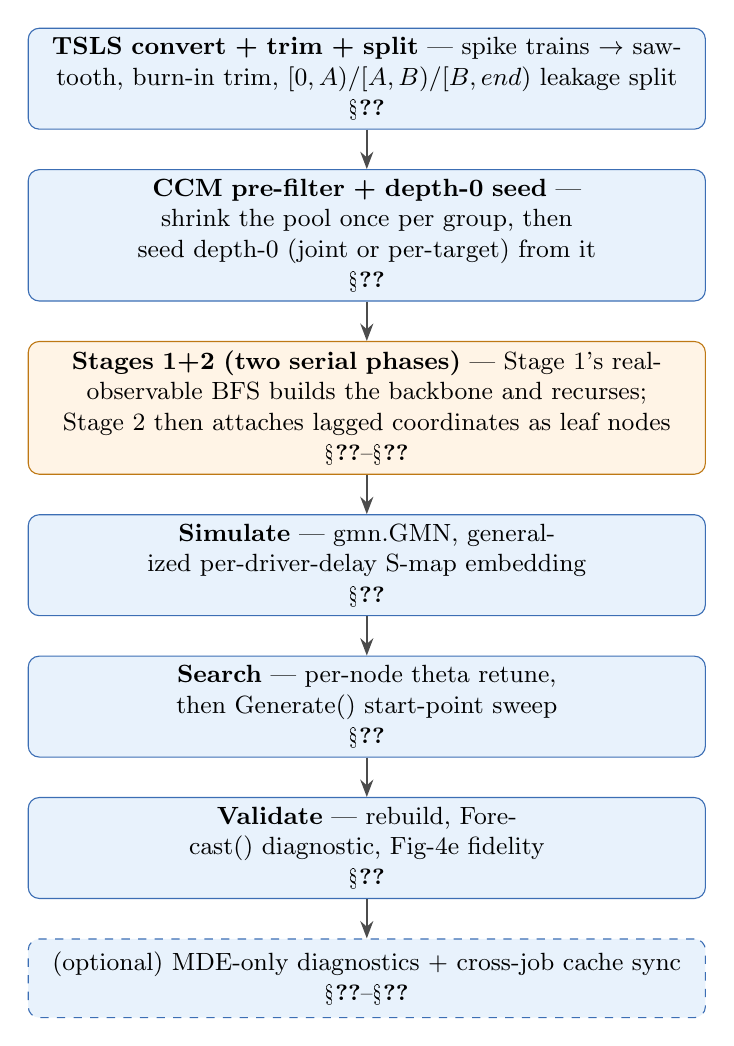
\begin{tikzpicture}[node distance=5mm]
  \node[stagebox] (s0) {\textbf{TSLS convert + trim + split} --- spike trains $\to$ sawtooth, burn-in trim, $[0,A){/}[A,B){/}[B,end)$ leakage split\\ \footnotesize \S\ref{sec:split}};
  \node[stagebox, below=of s0] (spre) {\textbf{CCM pre-filter + depth-0 seed} --- shrink the pool once per group, then seed depth-0 (joint or per-target) from it\\ \footnotesize \S\ref{sec:gmn-mode-joint}};
  \node[stage2box, below=of spre] (s1) {\textbf{Stages 1+2 (two serial phases)} --- Stage 1's real-observable BFS builds the backbone and recurses; Stage 2 then attaches lagged coordinates as leaf nodes\\ \footnotesize \S\ref{sec:stage1}--\S\ref{sec:stage2}};
  \node[stagebox, below=of s1] (s3) {\textbf{Simulate} --- gmn.GMN, generalized per-driver-delay S-map embedding\\ \footnotesize \S\ref{sec:smap}};
  \node[stagebox, below=of s3] (s4) {\textbf{Search} --- per-node theta retune, then Generate() start-point sweep\\ \footnotesize \S\ref{sec:search}};
  \node[stagebox, below=of s4] (s5) {\textbf{Validate} --- rebuild, Forecast() diagnostic, Fig-4e fidelity\\ \footnotesize \S\ref{sec:validation}};
  \node[stagebox, below=of s5, dashed] (s6) {(optional) MDE-only diagnostics + cross-job cache sync\\ \footnotesize \S\ref{sec:diagnostics}--\S\ref{sec:storage}};
  \foreach \a/\b in {s0/spre,spre/s1,s1/s3,s3/s4,s4/s5,s5/s6}
    \draw[arrow] (\a) -- (\b);
\end{tikzpicture}
\caption{The pipeline's stages, in \texttt{main()}'s actual call order. The orange box (unified Stages 1+2) is the nested-MDE network-discovery contribution ported from \texttt{simple-mde-gmn.py} -- see Section~\ref{sec:stage1}.}
\label{fig:overview}
\end{figure}

\subsection{Relationship to the sibling pipeline}
\label{sec:sibling}
\texttt{tsls-mde-gmn.py} and \texttt{simple-mde-gmn.py} (documented separately, \texttt{docs/simple-mde-gmn-pipeline.pdf}) began as deliberate, near-verbatim-duplicated siblings running the same CCM-pre-filter $\to$ two-phase nested-MDE $\to$ leaf-partitioning $\to$ generalized-embedding $\to$ S-map $\to$ theta/start-point search $\to$ validate architecture, kept as separate files rather than a shared module so that neither could silently break the other. The accepted cost was that a fix in one's shared machinery had to be ported by hand to the other -- and that cost came due: a defect was fixed in this pipeline and not in its then-duplicate, which is the direct reason the duplication was finally removed here (Section~\ref{sec:history-duplication}).

\textbf{They are no longer duplicates.} This pipeline's shared machinery now lives in the \texttt{mde\_gmn} package (Section~\ref{sec:architecture}), and its network algorithm has since changed in ways the sibling deliberately did not follow: a lagged pick is a leaf node here (Section~\ref{sec:stage2-leaves}), cycle-closing candidates are excluded before the MDE call rather than rejected after it (Section~\ref{sec:stage1-algo}), and Stage 2 is lagged-only. \texttt{simple-mde-gmn.py} keeps the older behaviour on purpose; it is a 1\,Hz pipeline with its own calibration, and changing it was explicitly out of scope. Read it as a related pipeline, not as this one's twin. Four deliberate asymmetries predate that split:
\begin{itemize}
  \item \textbf{Data representation.} \textbf{This pipeline TSLS-converts} every candidate neuron (Time Since Last Spike -- a continuous re-encoding of a spike train, since Takens embedding needs local geometry a sparse spike train doesn't have, Section~\ref{sec:split}) before anything else happens. The sibling pipeline does not -- it hands its MDE engine raw, per-region-binned spike \emph{counts} directly.
  \item \textbf{Selection/scoring engine.} \textbf{This pipeline uses \texttt{proper\_mde}/\texttt{proper\_ccm}} (\texttt{cleaned\_helper\_functions.py}, Sections~\ref{sec:mde-engine}--\ref{sec:ccm}), a from-scratch engine built so its internal scoring is pluggable -- event-timing-aware (\texttt{'f1'}/\texttt{'gamma'}) metrics for TSLS-converted neuron columns, plain correlation for continuous behavioral targets (Section~\ref{sec:scoring}). The sibling pipeline still calls the original third-party \texttt{dimx.MDE} (Pearson correlation scoring only). This asymmetry also has a downstream consequence for one parameter: \texttt{EXCLUSION\_RADIUS} is a dynamic, per-call \texttt{'auto'} mode in the sibling (it can intercept \texttt{dimx.Run}'s own staged internal calls) but a plain static integer here -- \texttt{proper\_mde} is one opaque call per dimension, with no internal staging to hook into (Section~\ref{sec:exclusion-radius}).
  \item \textbf{Joint (multi-target) depth-0 MDE seed.} \textbf{This pipeline} can replace its depth-0 MDE seed with a single, joint \texttt{multi\_proper\_mde} call across every \texttt{TARGETS} entry at once when \texttt{GMN\_MODE='combined'} (Section~\ref{sec:gmn-mode-joint}) -- forward-selecting drivers that jointly predict the whole group, rather than one independent \texttt{proper\_mde} call per target. The sibling pipeline has no such option: its own \texttt{GMN\_MODE='combined'} only ever affects network-sharing (one graph for every target vs.\ one per target); the underlying \texttt{dimx.MDE} selection call there is always per-target, regardless of \texttt{GMN\_MODE}.
  \item \textbf{The MDE-vs-baselines diagnostic.} This pipeline has its own TSLS-aware \texttt{run\_mde\_evaluate} (Section~\ref{sec:mde-evaluate}), built from scratch against \texttt{proper\_simplex}/\texttt{sklearn}/\texttt{pydiffmap} rather than the sibling's \texttt{dimx.Evaluate}-based one -- independent implementations of the same comparison, not a shared call path. Unlike the sibling's, this one is off by default, pending the diagnosis described in that section.
\end{itemize}
What the two still have in common, from the shared ancestry: the CCM pre-filter and depth-0 seeding order (Section~\ref{sec:gmn-mode-joint}), the overall two-phase backbone-then-lags shape (Sections~\ref{sec:stage1}--\ref{sec:stage2}), the leaf-partitioning/external-input design (Section~\ref{sec:partition}), the generalized per-driver-delay S-map embedding (Section~\ref{sec:smap}), the theta-only search plus generate-start sweep (Section~\ref{sec:search}), the three validation diagnostics (Section~\ref{sec:validation}), and the fingerprinted cross-job caching and storage architecture (Sections~\ref{sec:reuse}--\ref{sec:storage}). The details of the first two now differ, as above.

\subsection{How to read this document}
\begin{itemize}
  \item Each algorithm section opens with a plain-English statement of the problem being solved, then a numbered \textbf{Step 1 / Step 1.1 / Step 2 \ldots} breakdown of exactly what the code does, in order, using the exact function names in the \texttt{mde\_gmn} package (or \texttt{cleaned\_helper\_functions.py} where noted). Section~\ref{sec:architecture} says which module each name lives in.
  \item \tikz\node[draw=linknote, fill=linknote!6, rounded corners, inner sep=2pt]{\scriptsize\textbf{purple boxes}}; explain \emph{why} the next algorithm follows the one just described.
  \item \tikz\node[draw=badline, fill=badfill, rounded corners, inner sep=2pt]{\scriptsize\textbf{red boxes}}; flag a known risk, limitation, or open question.
  \item \tikz\node[draw=okline, fill=okfill, rounded corners, inner sep=2pt]{\scriptsize\textbf{green boxes}}; record a design decision made deliberately, with the reasoning, so it reads as a choice rather than an accident.
  \item Section~\ref{sec:outputs} is real output from actual runs of \emph{this exact codebase} -- not a mockup, not the sibling pipeline's output, and not a hypothetical. Section~\ref{sec:history} is the single most important section for a reviewer: a chronological, no-spin account of every bug this pipeline hit -- both in its original TSLS-specific engineering and in the more recent architectural port -- what was actually wrong, and what tradeoff each fix accepted.
\end{itemize}

\newpage
% =====================================================================
\section{Where the Code Lives}
\label{sec:architecture}
% =====================================================================

Everything this document describes is in the \texttt{mde\_gmn} package, one module per stage. The entry script is about forty lines: it puts its own directory on \texttt{sys.path}, imports the package, and calls \texttt{main()}. Every function named in the sections that follow lives in exactly one of these modules.

\begin{center}
\small
\begin{tabular}{@{}lll@{}}
\toprule
\textbf{Module} & \textbf{Stage} & \textbf{Covered in} \\
\midrule
\texttt{config.py}         & every \texttt{TSLS\_MDE\_GMN\_*} knob, read once & Appendix A \\
\texttt{pipeline.py}       & \texttt{main()} -- the run, step by step          & \S\ref{sec:e2e} \\
\texttt{tsls\_data.py}     & 0. TSLS conversion, burn-in trim, window sizing   & \S\ref{sec:split}, \S\ref{sec:window-sizing} \\
\texttt{mde.py}            & 1. forward selection + the CCM gate, per node     & \S\ref{sec:ccm-prefilter}, \S\ref{sec:mde-engine} \\
\texttt{network.py}        & 2. assembling the acyclic network                 & \S\ref{sec:stage1}--\S\ref{sec:partition} \\
\texttt{gmn\_build.py}     & 3. node dimensions and the \texttt{.cfg} for GMN  & \S\ref{sec:smap}, \S\ref{sec:gmn-mode} \\
\texttt{theta.py}          & 4. per-node $\theta$ tuning                       & \S\ref{sec:search} \\
\texttt{generate.py}       & 5. the free run, and scoring it                   & \S\ref{sec:validation} \\
\texttt{diagnostics.py}    & 6. optional baselines and sanity sweeps           & \S\ref{sec:diagnostics} \\
\texttt{gmn\_embedding.py} & the per-node embedding, and the \texttt{gmn} patches & \S\ref{sec:smap} \\
\texttt{columns.py}        & delay-suffixed column names                       & \S\ref{sec:stage2} \\
\texttt{caching.py}        & the cross-job cache and its fingerprints          & \S\ref{sec:reuse} \\
\texttt{progress.py}       & the heartbeat log                                 & \S\ref{sec:progress-log} \\
\texttt{plots.py}          & network figures                                   & \S\ref{sec:partition} \\
\bottomrule
\end{tabular}
\end{center}

A module only imports from modules above it in that list, so reading it top to bottom never requires a forward reference. \texttt{cleaned\_helper\_functions.py} -- the TSLS-aware EDM engine (\texttt{proper\_mde}, \texttt{proper\_ccm}, \texttt{proper\_simplex}) described in Sections~\ref{sec:mde-engine} and~\ref{sec:scoring} -- sits outside the package, because the batch scripts stage it as an individual file and the environment fingerprint hashes it by content.

\subsection{The parallel-MDE variant}
\label{sec:parallel-variant}
A second entry script, on the \texttt{no-kEDM-gpu-optimization} branch, runs the \emph{same} package with one substitution: \texttt{mde\_gmn/network\_parallel.py} in place of \texttt{network.py}. Everything else -- configuration, data, caching, GMN, $\theta$, scoring, output -- is shared code, so every section of this document applies to it unchanged except Sections~\ref{sec:stage1}--\ref{sec:stage2}, whose \emph{schedule} it alters.

The serial builder walks the graph breadth-first, and each wave ends in a barrier: every node in the wave must finish before the next wave can even be named, because what the next wave contains depends on what this one selected. With a handful of nodes per wave, most of the machine idles at every barrier. The parallel builder inverts that: \textbf{Phase 0} computes MDE for every node that could possibly be needed, all at once, with no barriers; \textbf{Phase 1} then walks the graph exactly as the serial builder does, but looks each answer up instead of computing it. More MDE calls are computed than the walk consults -- that is the trade, wasted compute bought with wall-clock.

\decisionbox{Where the parallel builder cannot simply look the answer up:}{Phase 0 cannot know which observables will end up upstream of a node, because "upstream" only exists once the graph is being built -- so a precomputed result can select a candidate that turns out to close a cycle. When the replay hits one, that node is recomputed serially with the offending candidates excluded, exactly as the serial builder's within-wave recompute does (Section~\ref{sec:stage1-algo}, step 7). Without it, the parallel builder would quietly accept networks the serial one would reject. \texttt{PARALLEL\_MDE\_SCOPE='staged'} reproduces the serial algorithm exactly, asserted edge for edge by \texttt{tests/test\_parallel\_mde\_equivalence.py}; \texttt{'union'} instead runs one combined MDE per node over real \emph{and} lagged candidates together, which is a different algorithm on purpose and so produces a different -- not a wrong -- network.}

\newpage
% =====================================================================
\section{Data Representation, Burn-In Trim, and the Three-Way Split}
\label{sec:split}
% =====================================================================

\subsection{Why not use raw spike counts directly?}
A spike train, sampled at 40\,Hz, is a sparse, mostly-zero series (a handful of 1s among thousands of 0s). Takens delay embedding -- the mathematical device every algorithm downstream depends on -- reconstructs a system's state space by stacking lagged copies of a single scalar signal into vectors. If that scalar signal is a spike count, the overwhelming majority of embedded points collapse onto the same ``no spike happening'' corner of the state space, leaving almost no usable geometric structure for nearest-neighbor-based prediction (Simplex/S-map) or causality testing (CCM) to exploit.

\textbf{TSLS (Time Since Last Spike)} recodes the same information losslessly as a continuous signal: it counts up linearly while no spike occurs, and drops back down to (near) zero the instant a new spike happens. The result is a sawtooth wave whose downward edges are, by construction, exactly the original spike times -- no information is discarded, but the signal now has genuine local geometry (slope, curvature, recent history) for a delay embedding to use.

\begin{figure}[h]
\centering
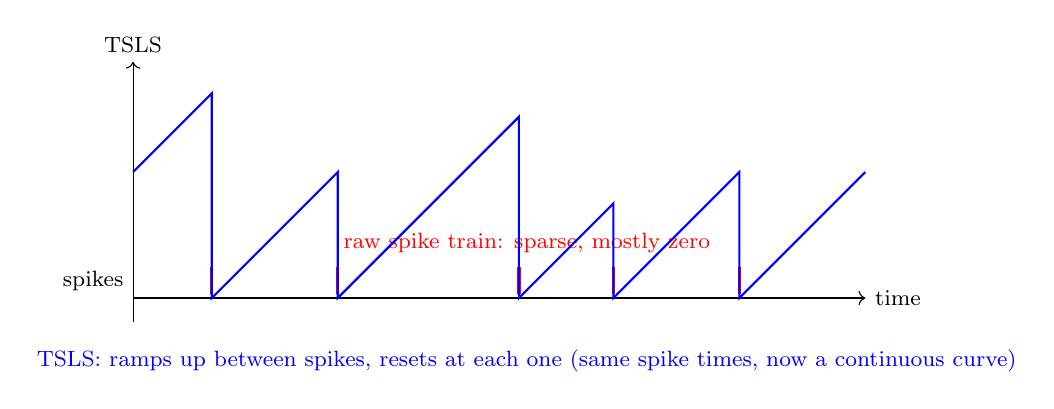
\begin{tikzpicture}[scale=1.0]
  \draw[->] (0,0) -- (9.3,0) node[right] {\footnotesize time};
  \foreach \x in {1,2.6,4.9,6.1,7.7} \draw[very thick, red] (\x,0.05) -- (\x,0.4);
  \node[left] at (0,0.22) {\footnotesize spikes};
  \node[align=center, red] at (5,0.7) {\footnotesize raw spike train: sparse, mostly zero};

  \draw[->] (0,-0.3) -- (0,3.0) node[above] {\footnotesize TSLS};
  \draw[blue, thick]
    (0,1.6) -- (1,2.6) -- (1,0) -- (2.6,1.6) -- (2.6,0)
    -- (4.9,2.3) -- (4.9,0) -- (6.1,1.2) -- (6.1,0)
    -- (7.7,1.6) -- (7.7,0) -- (9.3,1.6);
  \node[align=center, blue] at (5,-0.8) {\footnotesize TSLS: ramps up between spikes, resets at each one (same spike times, now a continuous curve)};
\end{tikzpicture}
\caption{TSLS conversion: the sawtooth's downward edges occur exactly at the original spike times.}
\label{fig:tsls-sawtooth}
\end{figure}

\subsection{Algorithm: \texttt{compute\_time\_since\_previous\_spike}}
\label{sec:algo-tsls-convert}
\textit{(cleaned\_helper\_functions.py)}
\begin{steps}
\item Take a sorted array of spike times for one channel, and a regular \texttt{time\_grid} (the recording's own bin centers) at which a TSLS value is wanted.
\item For every point \texttt{t} in \texttt{time\_grid}: select every spike time $\le$ \texttt{t}; if none exists yet (before this channel's first spike), record \texttt{NaN}; otherwise report \texttt{t} minus the most recent selected spike time.
\item Return one TSLS value per grid point, the same length as \texttt{time\_grid}.
\end{steps}
\pitfallbox{Cost note:}{This is an $O(N \times S)$ algorithm (boolean mask over all spikes, per grid point) with no vectorized shortcut -- for a channel with $S$ spikes and $N$ grid points, cost grows with both. Fast enough for this pipeline's per-channel-independent conversion at current scale, but would not scale gracefully to a much longer recording or higher firing rate without revisiting this loop.}

\subsection{Algorithm: \texttt{convert\_to\_tsls} and \texttt{burn\_in\_trim}}
\begin{steps}
\item \texttt{region\_neuron\_columns}/\texttt{raw\_neuron\_columns} select up to \texttt{REGION\_CHANNEL\_CAP} raw channels per region (CA1/mPFC/OFC).
\item \texttt{convert\_to\_tsls}: copy every \texttt{TARGETS} column (e.g.\ \texttt{head\_position\_x}, \texttt{head\_position\_y}) across \textbf{unchanged} -- continuous position measurements, never TSLS-converted; for every candidate neuron column, extract its spike times (rows where the raw count is $>0$) and run Step~\ref{sec:algo-tsls-convert} to get its \texttt{\{neuron\}\_tsls} series. Writes \texttt{tsls\_data\_full.csv}.
\item \texttt{burn\_in\_trim}: every TSLS column is \texttt{NaN} before that channel's own first spike. Find each candidate column's first non-\texttt{NaN} row, raise immediately if any channel never fires at all in the window, take the \emph{maximum} across channels (wait for the slowest-firing included channel), and drop every row before that point from the whole table -- targets included, so every column stays aligned to the same row index. Writes \texttt{tsls\_data\_trimmed.csv}.
\end{steps}
\decisionbox{Why trim eagerly rather than let downstream code mask NaN per-call:}{\texttt{cleaned\_helper\_functions.py}'s own \texttt{proper\_*} family masks \texttt{NaN} internally and would tolerate a little leading \texttt{NaN} -- but \texttt{gmn.GMN}'s own \texttt{Generate()}/\texttt{Forecast()} S-map calls (Section~\ref{sec:smap}) need one fully non-\texttt{NaN} table for the whole library/prediction range, and this pipeline's own delay-expansion step (\texttt{expand\_delay\_columns}, Section~\ref{sec:stage2}) reintroduces leading \texttt{NaN} of its own further downstream regardless. One eager, whole-table trim removes this entire class of risk at the cost of some usable data, rather than requiring every future consumer to independently remember the same NaN convention (see the PCA warm-up-row history entry, Section~\ref{sec:history-pca}, for what happens when a consumer doesn't).}
\pitfallbox{Cost of this design:}{A single very-slow-to-fire channel in the candidate pool determines how much data every other channel and both targets lose, regardless of how fast the other candidates are. With \texttt{REGION\_CHANNEL\_CAP} allowing many channels into the pool, one straggler can burn a meaningful fraction of the recording -- \texttt{"slowest channel to fire"} is printed to the job log for exactly this reason.}

\subsection{The leakage problem the three-way split solves}
\label{sec:leakage-problem}
Every stage after this one either (a) discovers which neurons causally drive the targets (Stages 1--2), or (b) reports how well a network simulates the targets' future (Sections~\ref{sec:search}--\ref{sec:validation}). If the same rows of data are used for both, the reported fidelity is not a genuine out-of-sample test. \texttt{load\_config()} and \texttt{main()} resolve one dataset-wide split, up front -- computed against the row count \emph{after} TSLS conversion and burn-in trim, since the usable window is itself data-driven (depends on which channel fires slowest), not a constant -- and every downstream stage is threaded through it.

\begin{figure}[h]
\centering
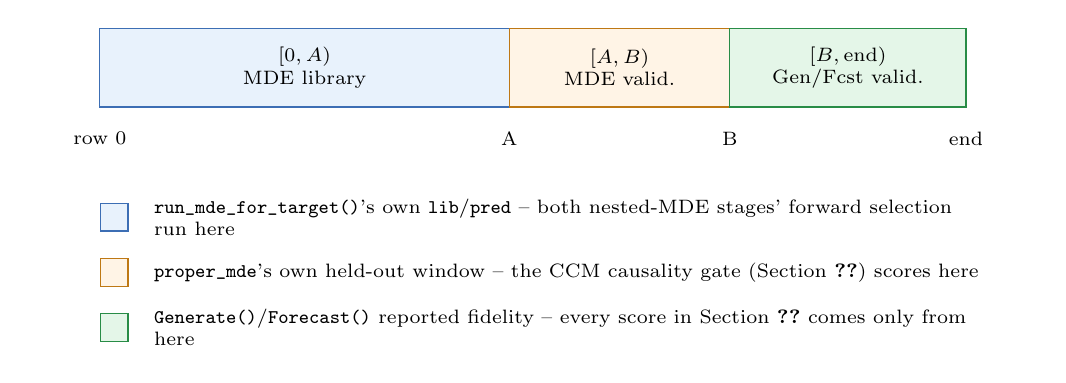
\begin{tikzpicture}[scale=1.0, every node/.style={font=\scriptsize}]
  \draw[fill=stagefill, draw=stageline] (0,0) rectangle (5.2,1);
  \node[align=center, text width=4.8cm] at (2.6,0.5) {$[0,A)$\\MDE library};
  \draw[fill=stage2fill, draw=stage2line] (5.2,0) rectangle (8.0,1);
  \node[align=center, text width=2.6cm] at (6.6,0.5) {$[A,B)$\\MDE valid.};
  \draw[fill=okfill, draw=okline] (8.0,0) rectangle (11.0,1);
  \node[align=center, text width=2.8cm] at (9.5,0.5) {$[B,\mathrm{end})$\\Gen/Fcst valid.};
  \node[below, text width=1.6cm, align=center] at (0,-0.2) {row 0};
  \node[below, text width=2.4cm, align=center] at (5.2,-0.2) {A};
  \node[below, text width=1.6cm, align=center] at (8.0,-0.2) {B};
  \node[below, text width=1.6cm, align=center] at (11.0,-0.2) {end};

  \node[rectangle, draw=stageline, fill=stagefill, minimum width=0.35cm, minimum height=0.35cm, anchor=west] (leg1) at (0,-1.4) {};
  \node[align=left, text width=10.6cm, anchor=west] at ($(leg1.east)+(0.2,0)$) {\texttt{run\_mde\_for\_target()}'s own \texttt{lib}/\texttt{pred} -- both nested-MDE stages' forward selection run here};
  \node[rectangle, draw=stage2line, fill=stage2fill, minimum width=0.35cm, minimum height=0.35cm, anchor=west] (leg2) at (0,-2.1) {};
  \node[align=left, text width=10.6cm, anchor=west] at ($(leg2.east)+(0.2,0)$) {\texttt{proper\_mde}'s own held-out window -- the CCM causality gate (Section~\ref{sec:mde-ccm-gate}) scores here};
  \node[rectangle, draw=okline, fill=okfill, minimum width=0.35cm, minimum height=0.35cm, anchor=west] (leg3) at (0,-2.8) {};
  \node[align=left, text width=10.6cm, anchor=west] at ($(leg3.east)+(0.2,0)$) {\texttt{Generate()}/\texttt{Forecast()} reported fidelity -- every score in Section~\ref{sec:validation} comes only from here};
\end{tikzpicture}
\caption{The three-way split: \texttt{PREDICTION\_START}=A $= \texttt{LIB\_RATIO} \times \mathrm{len(trimmed\ df)}$, \texttt{PREDICTION\_LENGTH}=B$-$A, \texttt{GENERATE\_VALIDATION\_START}=B. Network construction (Stages 1--2) never sees past B; every Generate()/Forecast() score is computed only on $[B, \mathrm{end})$.}
\label{fig:split}
\end{figure}

\subsection{Algorithm: the split's own arithmetic (\texttt{main()})}
\begin{steps}
\item \texttt{PREDICTION\_START} (A) $= \mathrm{round}(\texttt{LIB\_RATIO} \times \texttt{len(trimmed\ df)})$.
\item \texttt{PREDICTION\_LENGTH} (B$-$A) $= \mathrm{round}((\texttt{len(df)} - A) \times \texttt{MDE\_VALIDATION\_RATIO})$.
\item \texttt{GENERATE\_VALIDATION\_START} (B) $= A + (B{-}A)$; \texttt{GENERATE\_VALIDATION\_LENGTH} $= \texttt{len(df)} - B$.
\item \texttt{GENERATE\_LENGTH} (how many steps one \texttt{Generate()} call free-runs): $\le 0$ means "use the whole $[B,\mathrm{end})$ segment"; anything larger than \texttt{GENERATE\_VALIDATION\_LENGTH} is clamped down to it.
\end{steps}
\pitfallbox{\texttt{GENERATE\_LENGTH}'s resolved value feeds Stage 2's lag bound too -- not just Generate() length:}{\texttt{LAG\_MODE=generation\_length\_adjusted} (Section~\ref{sec:stage2}) ties Stage 2's deepest candidate lag to \texttt{GENERATE\_LENGTH} \emph{after} its own $\le 0$ sentinel has already resolved to the full held-out window (Step 4 above) -- caught during this project's own first cluster calibration run (Section~\ref{sec:history-generate-length}): leaving \texttt{GENERATE\_LENGTH} at its default would have silently expanded Stage 2's candidate pool to thousands of lag columns per real observable even with \texttt{REGION\_CHANNEL\_CAP}/\texttt{MDE\_D} capped small. Any deliberately small/calibration-scale run must cap \texttt{GENERATE\_LENGTH} explicitly, not rely on \texttt{REGION\_CHANNEL\_CAP}/\texttt{MDE\_D} alone -- or avoid the coupling altogether with \texttt{DELAY\_SOURCE=tau\_count} (Section~\ref{sec:lag-set}), which states the lag count directly and leaves \texttt{GENERATE\_LENGTH} meaning only what its name says.}

\subsection{Algorithm: \texttt{run\_mde\_for\_target}'s own leakage guard}
\label{sec:leakage-guard}
\begin{steps}
\item Slice \texttt{mde\_df = df[[target] + observable\_columns].iloc[:A + (B{-}A)]} -- physically truncate the DataFrame at row B before it is ever handed to \texttt{proper\_mde}.
\item Compute \texttt{warmup = max(|d| for d in delay\_set)} (the deepest delay-expansion column still needs that many valid rows before it) and skip that many rows at the front; also trim \texttt{tp} rows off the back (\texttt{B{-}tp}, not B), so the last validated row's own $t{+}\texttt{Tp}$ label can never land at or past B.
\item Both trims happen \emph{before} the row count is further bounded to this node's own resolved ranking window (\texttt{MIN\_PRED\_EVENTS}/\texttt{MAX\_WINDOW\_ROWS}, Section~\ref{sec:window-sizing} -- a fixed \texttt{TARGET\_RANKING\_WINDOW\_ROWS} for a behavioral target, a per-node event-count-driven window for a neuron) for \texttt{proper\_mde}'s own internal CCM sweep -- so that windowing can never reach back into $[B,\mathrm{end})$ regardless of its own size.
\end{steps}
\decisionbox{Physical truncation, not just lib/pred arguments:}{\texttt{mde\_df} is truncated as an object, not merely passed \texttt{lib}/\texttt{pred} range arguments that a callee could in principle ignore -- the same defense-in-depth reasoning as the sibling pipeline's own leakage guard against \texttt{dimx.MDE}'s internal \texttt{CCM()} call (which was confirmed, by reading \texttt{pyEDM} directly, to sample from whatever DataFrame it is handed regardless of the \texttt{lib}/\texttt{pred} strings). \texttt{proper\_mde} is this project's own code and does respect its \texttt{lib}/\texttt{pred} arguments, but the physical truncation is kept anyway as the same belt-and-suspenders guard, not removed just because the newer engine is trusted more.}

\linknote{Every row from 0 to B is now available for MDE to search (Stages 1--2 next), and every row from B onward is guaranteed untouched until the Generate()/Forecast() validation stages (Section~\ref{sec:validation}) -- exactly the property a genuine out-of-sample causal-network test needs.}

\newpage
% =====================================================================
\section{Before Stage 1: the CCM Pre-Filter and the Depth-0 MDE Seed}
\label{sec:gmn-mode-joint}
% =====================================================================
Two things happen in \texttt{main()} after the leakage-safe split (Section~\ref{sec:split}) but before Stage 1's BFS (Section~\ref{sec:stage1}) ever runs: the candidate pool is shrunk by a cheap CCM screen, and each target's own depth-0 driver search is seeded -- either independently or jointly, depending on \texttt{GMN\_MODE}. Both are explicit, main()-level steps for the same underlying reason: neither is something the BFS's own generic, per-node machinery can do on its own.

\subsection{The CCM pre-filter: shrinking the candidate pool before any MDE runs}
\label{sec:ccm-prefilter}
\texttt{REGION\_CHANNEL\_CAP} can offer hundreds of TSLS-converted channels as MDE candidates -- \texttt{proper\_mde}'s own forward-selection ranking cost grows with candidate-pool size at every dimension, so a large pool is expensive well before any driver is actually selected. \texttt{ccm\_prefilter\_observables()} runs a single, cheap CCM(observable $\to$ target) skill check per candidate, once per \texttt{target\_groups\_for\_mode()} group, and keeps only the candidates that cross-map at least one target in the group above \texttt{CCM\_PREFILTER\_RHO\_MIN} -- a coarse relevance screen, not a substitute for \texttt{proper\_mde}'s own causality-gated selection (Section~\ref{sec:mde-engine}).

\begin{steps}
\item For every group from \texttt{target\_groups\_for\_mode()}, window the library segment $[0,A)$ down to \texttt{CCM\_WINDOW\_ROWS} (the same bounded window every other CCM call in this pipeline uses, Section~\ref{sec:calibration}), and convert \texttt{LIBSIZE\_RATIOS} (fractions of that window) into actual library sizes.
\item For every (candidate, target) pair in the group, run one \texttt{proper\_ccm} at a static \texttt{CCM\_PREFILTER\_E} (no per-candidate auto-select -- would defeat the point of a \emph{cheap} filter) and average its score across the swept library sizes.
\item Average each candidate's per-target scores across the group; keep the candidate if that average is $\geq$ \texttt{CCM\_PREFILTER\_RHO\_MIN}. \texttt{CCM\_PREFILTER\_RHO\_MIN=0} disables the filter entirely (the pool passes through unchanged).
\item Parallelized over (candidate, target) pairs via a \texttt{ThreadPoolExecutor} -- \texttt{proper\_ccm}'s compiled KD-tree calls release the GIL, the same reasoning \texttt{run\_mde\_for\_target()}'s own inner pool already relies on.
\end{steps}

\begin{figure}[H]
\centering
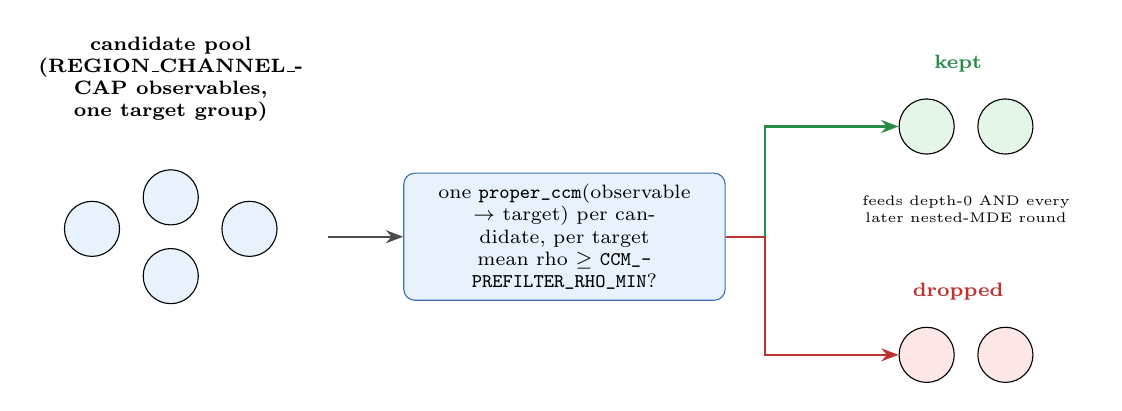
\begin{tikzpicture}[every node/.style={font=\scriptsize}]
  \node[font=\bfseries\scriptsize, align=center, text width=3.4cm] at (-4.6,3.3) {candidate pool\\(REGION\_CHANNEL\_CAP observables, one target group)};
  \node[circle, draw, fill=stagefill, minimum size=7mm] (o1) at (-5.6,1.4) {};
  \node[circle, draw, fill=stagefill, minimum size=7mm] (o2) at (-4.6,1.8) {};
  \node[circle, draw, fill=stagefill, minimum size=7mm] (o3) at (-3.6,1.4) {};
  \node[circle, draw, fill=stagefill, minimum size=7mm] (o4) at (-4.6,0.8) {};
  \node[smallbox, text width=3.8cm] (filt) at (0.4,1.3) {one \texttt{proper\_ccm}(observable $\to$ target) per candidate, per target\\mean rho $\geq$ \texttt{CCM\_PREFILTER\_RHO\_MIN}?};
  \draw[arrow] (-2.6,1.3) -- (filt);
  \node[font=\bfseries\scriptsize, okline] at (5.4,3.5) {kept};
  \node[circle, draw, fill=okfill, minimum size=7mm] (k1) at (5.0,2.7) {};
  \node[circle, draw, fill=okfill, minimum size=7mm] (k2) at (6.0,2.7) {};
  \node[font=\tiny, align=center, text width=3.0cm] at (5.5,1.65) {feeds depth-0 AND every later nested-MDE round};
  \draw[arrow, okline] (filt.east) -- ++(0.5,0) |- (k1);
  \node[font=\bfseries\scriptsize, badline] at (5.4,0.6) {dropped};
  \node[circle, draw, fill=badfill, minimum size=7mm] (d1) at (5.0,-0.2) {};
  \node[circle, draw, fill=badfill, minimum size=7mm] (d2) at (6.0,-0.2) {};
  \draw[arrow, badline] (filt.east) -- ++(0.5,0) |- (d1);
\end{tikzpicture}
\caption{\texttt{ccm\_prefilter\_observables()}: a coarse, cheap CCM relevance screen run once per target group, before depth-0 or any nested-MDE round ever searches the pool.}
\label{fig:ccm-prefilter}
\end{figure}

\subsection{Why depth-0 has to be computed explicitly, right here}
\label{sec:why-depth0-explicit}
\texttt{build\_nested\_mde\_network()}'s BFS (Section~\ref{sec:stage1}) is a generic, per-\emph{node} algorithm: every node it processes, target or driver alike, goes through the identical per-wave machinery, with one deliberate shortcut -- reuse a precomputed result instead of calling \texttt{proper\_mde} again when \texttt{depth==0 and node in mde\_results}. That shortcut is what makes depth-0 special, and it is also exactly why depth-0 cannot simply be left for the BFS to discover on its own the first time it reaches a target node, rather than diving straight from the CCM pre-filter into network construction.

\begin{steps}
\item The CCM pre-filter (Section~\ref{sec:ccm-prefilter}) is a \emph{group}-level operation -- it has to run once per \texttt{target\_groups\_for\_mode()} group, against every target in that group at once, before any individual node's MDE call happens. The BFS itself has no group-level entry point: it only ever sees one node at a time, so it has nowhere to run a once-per-group filter from.
\item Whatever pool that pre-filter produces has to be the \emph{same} pool every later round searches -- depth-0's own selection and every deeper nested-MDE round must all be choosing from identical candidates, or a column one round accepted can go missing from another round's own view of the universe.
\item \texttt{main()} therefore resolves \texttt{filtered\_pools[group]} once, up front, and passes that \emph{same} object both to the depth-0 seed call (\texttt{run\_mde\_for\_target}/\texttt{run\_multi\_mde\_for\_targets}) and to \texttt{build\_network()}'s own \texttt{observable\_columns} argument, which \texttt{build\_nested\_mde\_network()} then uses for every subsequent wave.
\end{steps}

\begin{figure}[H]
\centering
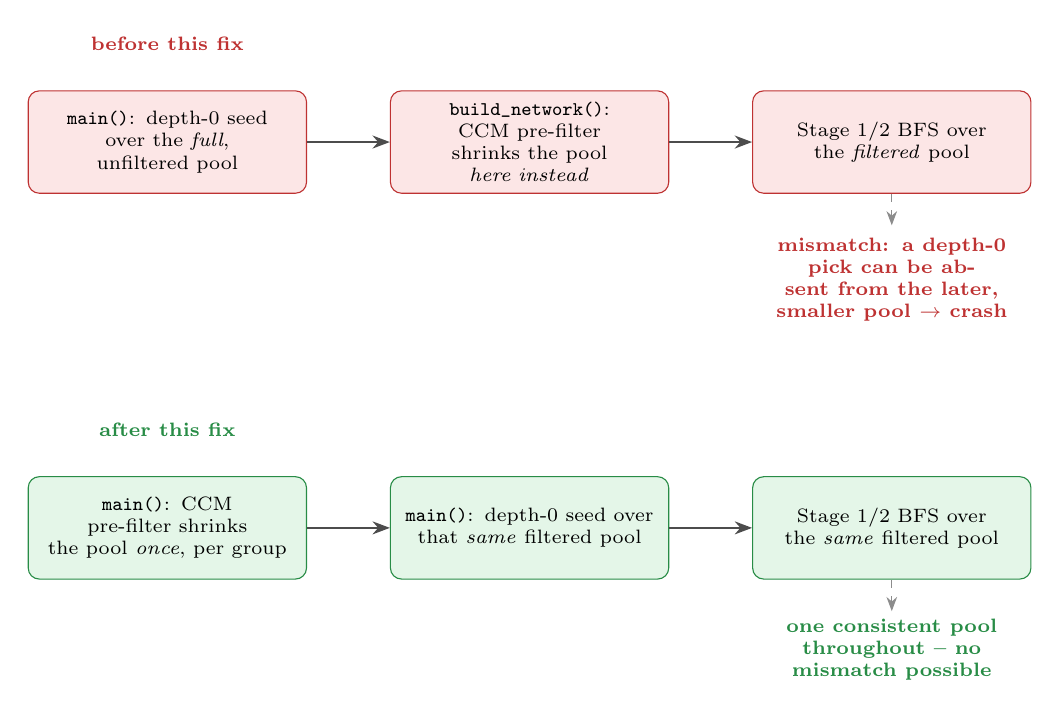
\begin{tikzpicture}[every node/.style={font=\scriptsize}]
  \node[font=\bfseries\scriptsize, badline] at (-5.6,3.75) {before this fix};
  \node[rectangle, draw=badline, fill=badfill, rounded corners, text width=3.3cm, minimum height=1.3cm, align=center] (old1) at (-5.6,2.5) {\texttt{main()}: depth-0 seed\\over the \emph{full}, unfiltered pool};
  \node[rectangle, draw=badline, fill=badfill, rounded corners, text width=3.3cm, minimum height=1.3cm, align=center] (old2) at (-1.0,2.5) {\texttt{build\_network()}: CCM pre-filter\\shrinks the pool \emph{here instead}};
  \node[rectangle, draw=badline, fill=badfill, rounded corners, text width=3.3cm, minimum height=1.3cm, align=center] (old3) at (3.6,2.5) {Stage 1/2 BFS over\\the \emph{filtered} pool};
  \draw[arrow] (old1) -- (old2);
  \draw[arrow] (old2) -- (old3);
  \draw[faintarrow] (old3.south) -- ++(0,-0.4);
  \node[font=\scriptsize\bfseries, badline, align=center, text width=3.4cm] at (3.6,0.75) {mismatch: a depth-0 pick can be absent from the later, smaller pool $\to$ crash};

  \node[font=\bfseries\scriptsize, okline] at (-5.6,-1.15) {after this fix};
  \node[rectangle, draw=okline, fill=okfill, rounded corners, text width=3.3cm, minimum height=1.3cm, align=center] (new1) at (-5.6,-2.4) {\texttt{main()}: CCM pre-filter shrinks\\the pool \emph{once}, per group};
  \node[rectangle, draw=okline, fill=okfill, rounded corners, text width=3.3cm, minimum height=1.3cm, align=center] (new2) at (-1.0,-2.4) {\texttt{main()}: depth-0 seed over\\that \emph{same} filtered pool};
  \node[rectangle, draw=okline, fill=okfill, rounded corners, text width=3.3cm, minimum height=1.3cm, align=center] (new3) at (3.6,-2.4) {Stage 1/2 BFS over\\the \emph{same} filtered pool};
  \draw[arrow] (new1) -- (new2);
  \draw[arrow] (new2) -- (new3);
  \draw[faintarrow] (new3.south) -- ++(0,-0.4);
  \node[font=\scriptsize\bfseries, okline, align=center, text width=3.4cm] at (3.6,-3.95) {one consistent pool throughout -- no mismatch possible};
\end{tikzpicture}
\caption{Reordering the CCM pre-filter fixed a real crash (\texttt{CA1\_12\_tsls}, Section~\ref{sec:history-prefilter-order}): depth-0's own candidate pool now comes from the exact same filtering pass every later nested-MDE round uses, instead of being computed separately, earlier, against a different (unfiltered) pool.}
\label{fig:prefilter-ordering}
\end{figure}

\pitfallbox{This is not a hypothetical failure mode -- it crashed real jobs:}{See Section~\ref{sec:history-prefilter-order} for the full symptom/investigation/decision writeup: \texttt{observable\_and\_delay()} raised \texttt{ValueError: invalid literal for int() with base 10: 'CA1\_12\_tsls'} when a depth-0-selected real observable, chosen against the old code's unfiltered pool, turned out absent from Stage 1/2's own (filtered) \texttt{raw\_columns} list.}

\subsection{What \texttt{GMN\_MODE} already controlled}
\texttt{target\_groups\_for\_mode()} groups \texttt{TARGETS} into either one list (\texttt{GMN\_MODE='combined'}, the default) or one singleton list per target (\texttt{'separate'}); \texttt{main()} then calls \texttt{build\_network()} once per group, so \texttt{'combined'} produces one shared graph spanning every target and \texttt{'separate'} produces one independent graph per target. Until this addition, that was \texttt{GMN\_MODE}'s \emph{only} effect: the depth-0 MDE seed feeding either mode was always computed identically -- one independent \texttt{proper\_mde} call per target (Section~\ref{sec:stage1}'s Step 1) -- regardless of how the resulting graphs were grouped downstream.

\subsection{What's new: a joint depth-0 seed under \texttt{'combined'}}
\texttt{GMN\_MODE='combined'} now \emph{also} changes how that depth-0 seed itself is computed (\texttt{MODE='MDE-GMN'} only -- \texttt{MODE='GMN'}'s interaction-matrix path, Section~\ref{sec:gmn-mode}, never calls MDE at all and is unaffected by any of this). Instead of \texttt{run\_mde\_for\_target()} once per target, \texttt{main()} calls a new wrapper, \texttt{run\_multi\_mde\_for\_targets()}, exactly \textbf{once} for the whole \texttt{TARGETS} group -- the only call site anywhere in the pipeline for \texttt{cleaned\_helper\_functions.multi\_proper\_mde}.

\begin{steps}
\item Build one candidate pool (every CCM-pre-filtered TSLS-converted observable, Section~\ref{sec:ccm-prefilter}, every target excluded) and one windowed \texttt{mde\_df} containing \emph{every} target column at once, not just one.
\item Run \texttt{multi\_proper\_mde}: at each forward-selection dimension, rank every remaining candidate by a Simplex prediction of \emph{each} target separately, then combine the per-target scores via \texttt{MULTI\_MDE\_TARGET\_AGGREGATE} (\texttt{'mean'} or \texttt{'min'}); CCM-gate survivors via \texttt{multi\_proper\_ccm}'s \texttt{t2c} direction -- the joint target manifold cross-mapped to the candidate neuron, the same causality convention as the single-target gate (Section~\ref{sec:mde-ccm-gate}), applied to the whole group at once.
\item The result is \textbf{one} shared \texttt{MDEcolumns} list and rho curve for the whole group -- there is no per-target breakdown, by construction: a driver was accepted because it predicts the \emph{group}, not any single target alone.
\item \texttt{main()} fans that single shared result out into one per-target \emph{view} in \texttt{mde\_results} (same underlying \texttt{SELECTED\_COLUMNS}/\texttt{m}/\texttt{mde\_df} object, just re-keyed with each target's own name) so every existing consumer that indexes \texttt{mde\_results[target]} -- Stage 1's depth-0 reuse, the MDE diagnostics plots (Section~\ref{sec:diagnostics}) -- keeps working completely unchanged.
\end{steps}

\begin{figure}[H]
\centering
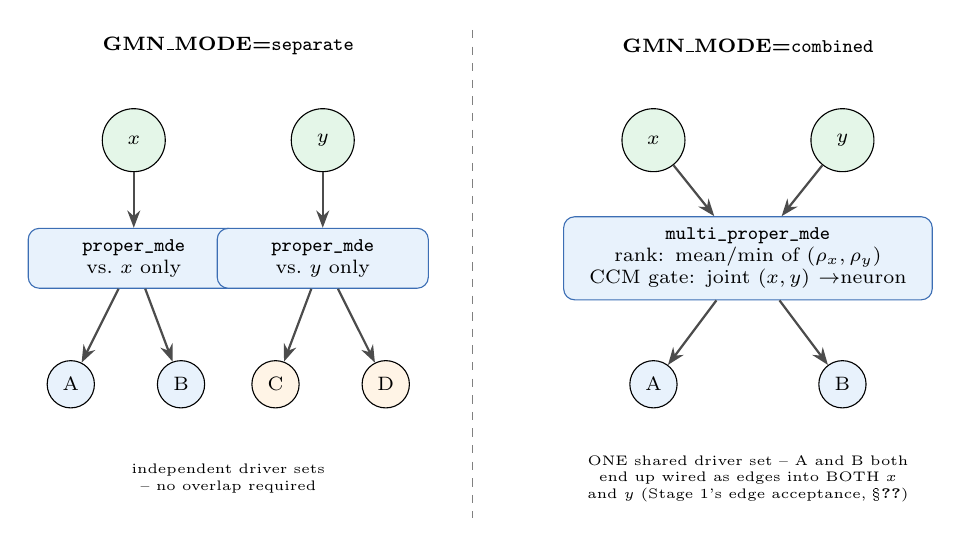
\begin{tikzpicture}[every node/.style={font=\scriptsize}]
  % ---- separate (left) ----
  \node[font=\bfseries\scriptsize] at (-3.2,4.6) {GMN\_MODE=\texttt{separate}};
  \node[circle, draw, fill=okfill, minimum size=8mm] (tx) at (-4.4,3.4) {$x$};
  \node[circle, draw, fill=okfill, minimum size=8mm] (ty) at (-2.0,3.4) {$y$};
  \node[smallbox, text width=2.4cm] (mx) at (-4.4,1.9) {\texttt{proper\_mde}\\vs.\ $x$ only};
  \node[smallbox, text width=2.4cm] (my) at (-2.0,1.9) {\texttt{proper\_mde}\\vs.\ $y$ only};
  \draw[arrow] (tx) -- (mx);
  \draw[arrow] (ty) -- (my);
  \node[circle, draw, fill=stagefill, minimum size=6mm] (dax) at (-5.2,0.3) {A};
  \node[circle, draw, fill=stagefill, minimum size=6mm] (dbx) at (-3.8,0.3) {B};
  \node[circle, draw, fill=stage2fill, minimum size=6mm] (day) at (-2.6,0.3) {C};
  \node[circle, draw, fill=stage2fill, minimum size=6mm] (dby) at (-1.2,0.3) {D};
  \draw[arrow] (mx) -- (dax);
  \draw[arrow] (mx) -- (dbx);
  \draw[arrow] (my) -- (day);
  \draw[arrow] (my) -- (dby);
  \node[font=\tiny, align=center, text width=4.6cm] at (-3.2,-0.9) {independent driver sets -- no overlap required};

  % ---- divider ----
  \draw[dashed, gray] (-0.1,4.8) -- (-0.1,-1.4);

  % ---- combined (right) ----
  \node[font=\bfseries\scriptsize] at (3.4,4.6) {GMN\_MODE=\texttt{combined}};
  \node[circle, draw, fill=okfill, minimum size=8mm] (gx) at (2.2,3.4) {$x$};
  \node[circle, draw, fill=okfill, minimum size=8mm] (gy) at (4.6,3.4) {$y$};
  \node[smallbox, text width=4.4cm] (mm) at (3.4,1.9) {\texttt{multi\_proper\_mde}\\rank: mean/min of $(\rho_x,\rho_y)$\\CCM gate: joint $(x,y)\to$neuron};
  \draw[arrow] (gx) -- (mm);
  \draw[arrow] (gy) -- (mm);
  \node[circle, draw, fill=stagefill, minimum size=6mm] (ga) at (2.2,0.3) {A};
  \node[circle, draw, fill=stagefill, minimum size=6mm] (gb) at (4.6,0.3) {B};
  \draw[arrow] (mm) -- (ga);
  \draw[arrow] (mm) -- (gb);
  \node[font=\tiny, align=center, text width=4.8cm] at (3.4,-0.9) {ONE shared driver set -- A and B both end up wired as edges into BOTH $x$ and $y$ (Stage 1's edge acceptance, \S\ref{sec:stage1})};
\end{tikzpicture}
\caption{The depth-0 seed under each \texttt{GMN\_MODE}, for two targets $x$, $y$: \texttt{'separate'} (left) ranks and CCM-gates each target independently, so the two can end up with entirely disjoint driver sets; \texttt{'combined'} (right) ranks and gates against the joint pair at once, producing one shared driver set wired identically into every target node.}
\label{fig:gmn-mode-joint}
\end{figure}

\subsection{New configuration: \texttt{MULTI\_MDE\_E} and \texttt{MULTI\_MDE\_TARGET\_AGGREGATE}}
\texttt{multi\_proper\_mde} has no per-candidate \texttt{EmbedDimension} auto-select path -- that is a single-target, Pearson-rho-only \texttt{pyEDM} routine (Section~\ref{sec:mde-ccm-gate}) -- so its CCM gate needs a static, explicit embedding dimension. \texttt{MULTI\_MDE\_E} (default \textbf{3}) supplies it; \texttt{MULTI\_MDE\_TARGET\_AGGREGATE} (default \textbf{\texttt{'mean'}}, or \texttt{'min'}) picks how per-target ranking/CCM scores are combined -- \texttt{'mean'} avoids penalizing a driver that is strong for one target and weak for another, \texttt{'min'} only accepts drivers simultaneously good for every target. Both are no-ops under \texttt{GMN\_MODE='separate'}.

\subsection{Scope: exactly one call site, depth 0 only}
\begin{figure}[H]
\centering
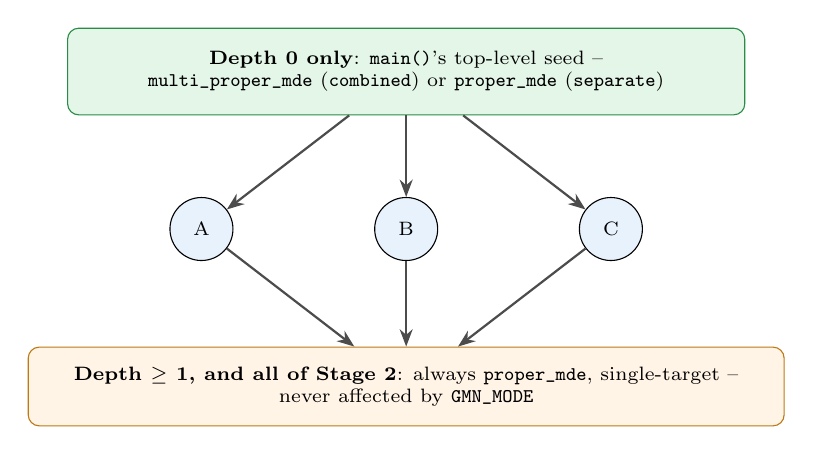
\begin{tikzpicture}[every node/.style={font=\scriptsize}]
  \node[rectangle, draw=okline, fill=okfill, rounded corners, minimum width=8.6cm, minimum height=1.1cm, align=center] (depth0) at (0,3.0) {\textbf{Depth 0 only}: \texttt{main()}'s top-level seed --\\ \texttt{multi\_proper\_mde} (\texttt{combined}) or \texttt{proper\_mde} (\texttt{separate})};
  \node[circle, draw, fill=stagefill, minimum size=8mm] (a) at (-2.6,1.0) {A};
  \node[circle, draw, fill=stagefill, minimum size=8mm] (b) at (0,1.0) {B};
  \node[circle, draw, fill=stagefill, minimum size=8mm] (c) at (2.6,1.0) {C};
  \draw[arrow] (depth0) -- (a);
  \draw[arrow] (depth0) -- (b);
  \draw[arrow] (depth0) -- (c);
  \node[rectangle, draw=stage2line, fill=stage2fill, rounded corners, minimum width=9.6cm, minimum height=1.0cm, align=center] (deeper) at (0,-1.0) {\textbf{Depth $\ge$ 1, and all of Stage 2}: always \texttt{proper\_mde}, single-target --\\ never affected by \texttt{GMN\_MODE}};
  \draw[arrow] (a) -- (deeper);
  \draw[arrow] (b) -- (deeper);
  \draw[arrow] (c) -- (deeper);
\end{tikzpicture}
\caption{\texttt{multi\_proper\_mde} is confined to exactly one call site: \texttt{main()}'s depth-0 seed, under \texttt{GMN\_MODE='combined'}. Every subsequent recursion level Stage 1 discovers (depth 1, 2, \ldots up to \texttt{NESTED\_M}), and all of Stage 2's per-node lag attachment, always uses the same single-target \texttt{proper\_mde} it used before \texttt{multi\_proper\_mde} was introduced -- a deliberate scope boundary, not an oversight.}
\label{fig:multi-mde-scope}
\end{figure}

\decisionbox{Why confined to depth 0 only:}{Depth 0 is the only place in the algorithm where "target" means one of \texttt{TARGETS} (an actual behavioral variable) -- every deeper node Stage 1's recursion discovers, and every node Stage 2 attaches lags to, is a \emph{neuron}, not a target: there is no "joint prediction of several neurons at once" question to ask there, and \texttt{run\_multi\_mde\_for\_targets()} is never called for one. Confirmed directly against the source: \texttt{multi\_proper\_mde} appears in exactly one call site in the whole file (\texttt{run\_multi\_mde\_for\_targets()}), itself called from exactly one place (\texttt{main()}'s depth-0 seed); \texttt{build\_nested\_mde\_network()}'s per-wave Stage 1 \emph{and} Stage 2 passes (Section~\ref{sec:stage1}) both still submit plain \texttt{run\_mde\_for\_target} by name, byte-for-byte unchanged from before this addition.}

\pitfallbox{Cache fingerprints had to be extended, not just the algorithm:}{\texttt{GMN\_MODE} and the two new knobs above now shape the depth-0 \texttt{mde\_results} that \texttt{build\_network()} is handed, even though \texttt{build\_network()} itself never calls \texttt{multi\_proper\_mde} -- so \texttt{build\_network\_fingerprint()} and \texttt{build\_search\_fingerprint()} (Section~\ref{sec:reuse}) now include \texttt{gmn\_mode}/\texttt{multi\_mde\_e}/\texttt{multi\_mde\_target\_aggregate} alongside \texttt{mde\_d}/\texttt{tp}/etc. Without this, a \texttt{REUSE\_BEST\_PARAMS} resubmission that only changed \texttt{GMN\_MODE} could silently reuse a stale cached network built from the other mode's own depth-0 seed.}

\linknote{Whichever way the depth-0 seed was computed, Stage 1 (next) receives it as an ordinary precomputed \texttt{mde\_results} entry and proceeds identically either way -- the BFS itself has no branch on \texttt{GMN\_MODE} at all.}

\newpage
% =====================================================================
\section{Stage 1: Nested-MDE Backbone Discovery}
\label{sec:stage1}
% =====================================================================

\subsection{Why this has no notebook precedent}
The reference notebook builds a network by running CCM over the \emph{union} of each target's MDE-selected columns, then handing an $N \times N$ interaction matrix to \texttt{apps.CreateNetwork} for greedy, acyclic graph assembly -- this pipeline's own \texttt{MODE='GMN'} branch still does exactly this (Section~\ref{sec:gmn-mode}), unaffected by anything in this section. \texttt{build\_nested\_mde\_network()} (\texttt{MODE='MDE-GMN'}, the default) replaces that approach for network construction proper: it discovers the network's topology directly from repeated \texttt{proper\_mde} calls -- no CCM interaction matrix, no \texttt{apps.CreateNetwork}. Each target's MDE-selected drivers themselves become new MDE targets, recursively, for \texttt{NESTED\_M} further rounds.

\subsection{Algorithm: \texttt{build\_nested\_mde\_network} -- two fully-serial BFS phases}
\label{sec:stage1-algo}
Stage 1 and Stage 2 share one function and one depth-budget accounting scheme, but -- as of R12 (2026-08-27, superseding the 2026-08-25 interleaved design this section described before) -- they are \textbf{not} interleaved wave-by-wave. \texttt{build\_nested\_mde\_network()} instead runs two fully sequential phases: \textbf{Phase 1 (Stage 1) runs its entire real-observable-only BFS to completion first} -- every depth the \texttt{NESTED\_M} budget allows -- \textbf{before Phase 2 (Stage 2) starts at all.} Phase 2 is then seeded with \emph{every} node Phase 1 discovered, at the depth Phase 1 discovered it, not with the targets alone -- this is what guarantees every Stage 1 backbone node still gets its own lagged/real embedding attachment, the same guarantee the old interleaving gave one wave at a time.
\begin{steps}
\item \textbf{Depth 0:} \texttt{main()} already computed \texttt{mde\_results} for every target before this function ever runs -- either one \texttt{proper\_mde} call per target (\texttt{GMN\_MODE='separate'}) or one joint \texttt{multi\_proper\_mde} call across the whole group (\texttt{GMN\_MODE='combined'}, Section~\ref{sec:gmn-mode-joint}), each selecting up to \texttt{MDE\_D} distinct real observables from the CCM-pre-filtered candidate pool (Section~\ref{sec:ccm-prefilter}, excluding the target(s) themselves). Phase 1 reuses that precomputed result as its own depth-0 round, rather than paying for it twice.
\item \textbf{Phase 1 (Stage 1), every wave:} a real-observable-only pass per not-yet-visited node (so every accepted edge necessarily has delay 0), via \texttt{run\_mde\_for\_target()}. Every driver selected \emph{at delay 0} becomes a new MDE target for the next wave, up to the \texttt{NESTED\_M} budget (\texttt{NESTED\_M=0} is a sentinel for "uncapped" -- Phase 1 terminates on its own once every reachable real observable in the finite candidate pool has been visited or every remaining branch dead-ends). Phase 1 runs to completion -- every depth, every wave -- before Phase 2 below ever starts.
\item \textbf{Phase 2 (Stage 2), one pass over Phase 1's final node set:} one \textbf{Stage 2 pass} per node Phase 1 visited (targets and every discovered backbone node alike). Candidates are \textbf{lagged columns only}, drawn from the whole CCM-pre-filtered observable universe -- every observable's lag embeddings, whether or not Stage 1 selected that observable. Each accepted pick becomes its own leaf node (Section~\ref{sec:stage2-leaves}), which is never expanded, so Phase 2 has no second wave and cannot deepen the network.
\item \textbf{Acyclicity is enforced \emph{before} the MDE call, not after it} (\texttt{\_real\_candidate\_pool()}). A Stage 1 node's candidate pool excludes the node itself and every observable already downstream of it in the graph -- \texttt{nx.descendants(node)}, since edges run driver $\to$ node, so a node's graph descendants are what "upstream of it causally" means. This matters because forward selection is greedy: a pick rejected \emph{after} selection has already consumed one of the node's \texttt{MDE\_D} driver slots and conditioned every later round, so the node ends up with fewer and worse drivers than if the illegal candidate had never been offered.
\item \textbf{Edge acceptance} (\texttt{\_accept\_mde\_result\_edges()}, shared by both phases): reject a self-loop at delay 0; reject a \texttt{NaN} marginal MDE rho gain; add a delay=0 pick as an edge from the real observable's own node, and a delay$\ne$0 pick as an edge from its own freshly created leaf node (Section~\ref{sec:stage2-leaves}). The \texttt{nx.is\_directed\_acyclic\_graph()} check now runs only for delay=0 edges, and a failure there is logged as \texttt{UNEXPECTED} -- with the pool exclusion above in place, it should be unreachable, so it is an assertion rather than part of the algorithm.
\item \textbf{Depth is recorded as a minimum.} A brand-new driver proposed by two parents in the same wave is enqueued at the \emph{shallowest} proposed depth, not whichever parent happens to be iterated first -- \texttt{next\_wave} is a \texttt{\{driver: min\_depth\}} dict, not a plain list, so a node's depth never depends on iteration order.
\item \textbf{The within-wave race, and the recompute that closes it.} A wave's candidate pools are all built \emph{before} any of that wave's results come back, so two nodes in one wave can each select the other: neither pool could have known, because neither edge existed yet. Whichever result is accepted second would close a cycle. That node is recomputed serially, with the other's edges now in the graph and its pool re-derived (\texttt{\_recomputed\_stage1\_result()}). Rejecting the edge instead would hit the same greedy-selection problem as step 4 -- which is why the recompute exists rather than a late rejection.
\end{steps}
\decisionbox{Why serialize, if the interleaved design already worked?}{Review (R12) found no correctness defect in the interleaved 2026-08-25 design -- both a Stage 1 and a Stage 2 real-observable pick already fed the next wave correctly. Serializing the two phases was a clarity/maintainability change: two independent \texttt{while} loops with their own \texttt{visited1}/\texttt{visited2} sets are easier to reason about (and to test -- \texttt{tests/test\_r12\_stage\_serialization.py} asserts every Stage 1 call in the invocation log precedes every Stage 2 call) than one loop juggling both passes' state per wave. Behaviorally the two designs agree on the node set discovered when the depth budget is `NESTED\_M`-limited on a branch, but not necessarily on parallelism grain, since Phase 2 now runs as its own separate wave-by-wave sweep after Phase 1 finishes rather than sharing Phase 1's own wave boundaries.}

\begin{figure}[h]
\centering
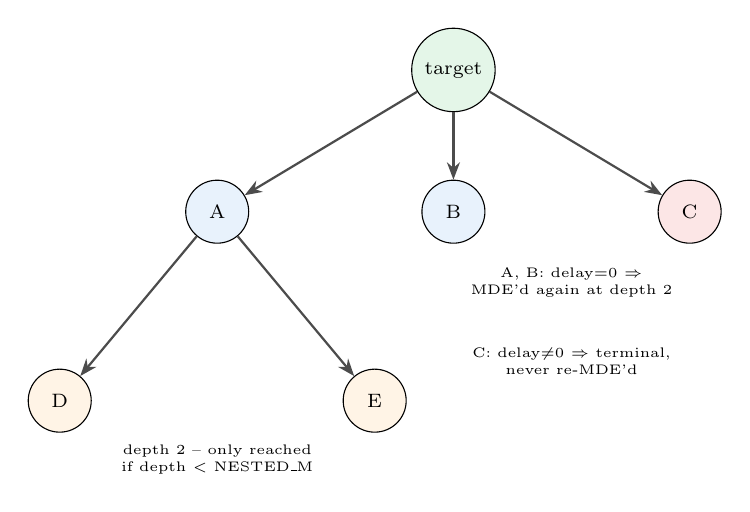
\begin{tikzpicture}[every node/.style={font=\scriptsize}]
  \node[circle, draw, fill=okfill, minimum size=8mm] (root) at (4.2,4.4) {target};
  \node[circle, draw, fill=stagefill, minimum size=8mm] (a) at (1.2,2.6) {A};
  \node[circle, draw, fill=stagefill, minimum size=8mm] (b) at (4.2,2.6) {B};
  \node[circle, draw, fill=badfill, minimum size=8mm] (c) at (7.2,2.6) {C};
  \draw[arrow] (root) -- (a);
  \draw[arrow] (root) -- (b);
  \draw[arrow] (root) -- (c);
  \node[font=\tiny, align=center, text width=2.6cm] at (5.7,1.7) {A, B: delay=0 $\Rightarrow$ MDE'd again at depth 2};
  \node[font=\tiny, align=center, text width=2.6cm] at (5.7,0.7) {C: delay$\ne$0 $\Rightarrow$ terminal, never re-MDE'd};
  \node[circle, draw, fill=stage2fill, minimum size=8mm] (d) at (-0.8,0.2) {D};
  \node[circle, draw, fill=stage2fill, minimum size=8mm] (e) at (3.2,0.2) {E};
  \draw[arrow] (a) -- (d);
  \draw[arrow] (a) -- (e);
  \node[font=\tiny, align=center, text width=3.8cm] at (1.2,-0.55) {depth 2 -- only reached if depth $<$ NESTED\_M};
\end{tikzpicture}
\caption{The BFS's depth/delay rule: only delay-0 accepted edges (A, B) enqueue their driver for further nesting. A nonzero-delay pick (C) is a leaf node of its own and terminates that branch immediately (Section~\ref{sec:stage2-leaves}). Since Stage 1 offers only delay-0 candidates and Stage 2 only lagged ones, the two cases correspond exactly to the two phases.}
\label{fig:stage1-bfs}
\end{figure}

\decisionbox{Why only delay=0 continues the search:}{A driver selected at a nonzero delay stands in for an unobserved dimension of the true state space -- a coordinate, per generalized embedding theory (Deyle \& Sugihara 2011), not a physical variable whose own causal history is worth discovering. A lagged pick is therefore a leaf: it is not simulated at all, but fed from the recorded data as an external input (Sections~\ref{sec:stage2-leaves} and~\ref{sec:partition}).}

\decisionbox{Why a \texttt{MultiDiGraph}, not a \texttt{DiGraph}:}{The same observable can drive one node at several different delays at once -- each is kept as its own separate edge, not deduplicated to one edge with one delay.}

\subsection{Algorithm: parallelization, outer and inner}
\label{sec:stage1-parallelization}
Every node at the same BFS depth is MDE-independent of every other, so each pass (Stage 1, then Stage 2) is submitted concurrently via its own \texttt{ProcessPoolExecutor}: \texttt{outer\_workers = min(len(wave), cores)}. \texttt{proper\_mde} itself has no multiprocessing of its own, but as of 2026-08-25 \texttt{run\_mde\_for\_target()} opens one additional \texttt{ThreadPoolExecutor} \emph{inside} each of those outer worker processes -- \texttt{inner\_workers = max(1, cores // outer\_workers)}, recomputed fresh per pass per wave from that pass's own real node count -- and passes it into \texttt{proper\_mde} as its own \texttt{pool} argument, reused across every forward-selection dimension's ranking loop and CCM-gate candidate for that one node. Threads, not another process pool, because every hot loop \texttt{proper\_mde} reaches (\texttt{pyEDM}/KD-tree calls) is a compiled routine that releases the GIL -- the same reasoning \texttt{ccm\_prefilter\_observables()}'s own thread pool (Section~\ref{sec:ccm-prefilter}) relies on. \texttt{outer\_workers} $\times$ \texttt{inner\_workers} $\leq$ \texttt{cores} always, by construction -- the same pool-squaring guard the sibling pipeline's own outer/inner CCM split already established (sibling document, "The nested-multiprocessing-pool blowup").

\begin{figure}[H]
\centering
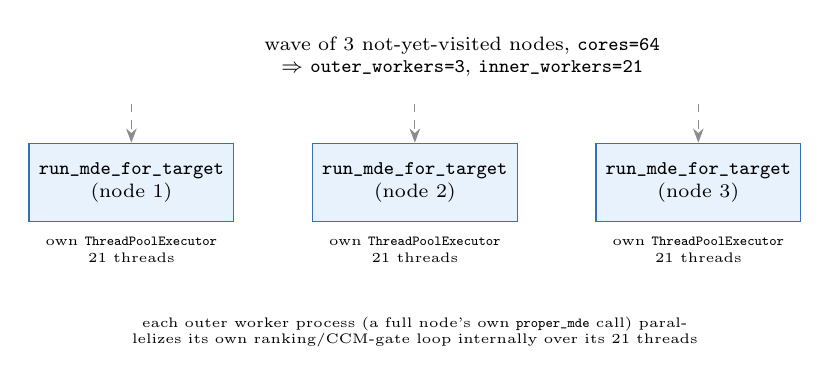
\begin{tikzpicture}[every node/.style={font=\scriptsize}]
  \node[align=center, text width=8cm] at (4.2,3.6) {wave of 3 not-yet-visited nodes, \texttt{cores=64}\\$\Rightarrow$ \texttt{outer\_workers=3}, \texttt{inner\_workers=21}};
  \foreach \i/\x in {1/0,2/3.6,3/7.2} {
    \node[rectangle, draw=stageline, fill=stagefill, minimum width=2.6cm, minimum height=1.0cm, align=center] (w\i) at (\x,2.0) {\texttt{run\_mde\_for\_target}\\(node \i)};
    \node[font=\tiny, align=center] at (\x,1.15) {own \texttt{ThreadPoolExecutor}\\21 threads};
    \draw[faintarrow] (\x,3.0) -- (w\i);
  }
  \node[font=\tiny, text width=9.6cm, align=center] at (3.6,0.1) {each outer worker process (a full node's own \texttt{proper\_mde} call) parallelizes its own ranking/CCM-gate loop internally over its 21 threads};
\end{tikzpicture}
\caption{One pass's own outer/inner split within a wave: 3 outer worker processes, each opening its own 21-thread inner pool for that one node's \texttt{proper\_mde} call -- $3 \times 21 = 63 \leq 64$ cores.}
\label{fig:stage1-inner-pool}
\end{figure}

\pitfallbox{A single degenerate node can still crash the entire job -- guarded the same way as the sibling pipeline:}{The sibling pipeline lost 1 day 11 hours of compute once to a single node's third-party MDE call hitting an all-NaN rho column, an exception that propagated out of the wave's \texttt{ProcessPoolExecutor} and killed every already-completed node's work alongside it (sibling document, "The all-NaN crash"). \texttt{proper\_mde} is this project's own code and has not been observed to hit that exact failure mode, but every wave-consumption loop here (both passes, and \texttt{main()}'s own depth-0 seed) still catches per-node exceptions and substitutes \texttt{\_failed\_mde\_result()} -- shaped identically to a legitimate zero-driver selection -- ported proactively rather than waiting to hit the same class of bug independently.}

\linknote{Phase 1 leaves behind a backbone of real observables, every edge at delay 0. What it does not yet say is how far back in time each node should look, or which lagged coordinates best explain it -- that is Section~\ref{sec:stage2}'s subject, and the form its answers take (leaf nodes, not annotated edges) is what makes them impossible to cycle.}

\newpage
% =====================================================================
\section{Stage 2: Lagged-Embedding Attachment}
\label{sec:stage2}
% =====================================================================

\subsection{The problem Stage 2 solves}
Stage 1's own picks tell you \emph{which} real observables matter and how they connect. They say nothing about \emph{how far back in time} each connection should look, or which additional variables -- not necessarily direct Stage-1 neighbors -- best explain a node's own recent history once its embedding is allowed to be genuinely non-uniform (a generalized/non-uniform Takens embedding, Deyle \& Sugihara 2011). Stage 2 runs exactly one \texttt{proper\_mde} round per node, once, to answer that.

\subsection{Algorithm: the Stage 2 pass}
\begin{steps}
\item For every node Stage 1 visited (targets included, at every depth), build a candidate pool of \texttt{lag\_set} $\times$ \emph{every} observable in the CCM-pre-filtered universe -- not restricted to that node's own Stage-1 neighbors, so a node's best lagged predictor can come from anywhere. The pool includes lagged copies of the node itself, of observables Stage 1 selected, and of observables Stage 1 never touched.
\item The pool is \textbf{lagged columns only}. Every candidate carries a nonzero delay; no delay=0 column is on offer. Stage 2 therefore cannot extend the real-observable backbone, and \texttt{NESTED\_M} governs Stage 1 alone.
\item Run one \texttt{proper\_mde} round (same \texttt{run\_mde\_for\_target()}, same leakage guard as Stage 1, \texttt{cache\_stage='stage2'} so its cache files never collide with Stage 1's) selecting up to \texttt{MDE\_D} lagged columns.
\item Feed every result through the \emph{same} \texttt{\_accept\_mde\_result\_edges()} as Stage 1. Each accepted lagged pick becomes its own \textbf{leaf node} -- see Section~\ref{sec:stage2-leaves}.
\item There is no second wave. Stage 2 is one pass over Stage 1's final node set, and it discovers no node that could need expanding.
\end{steps}
\decisionbox{Why Stage 2 is lagged-only:}{A delay$\ne$0 driver stands in for an unobserved dimension of the true state space -- a coordinate, per generalized embedding theory (Deyle \& Sugihara 2011), not a physical variable whose own causal history is worth discovering. Stage 1 already searches the real observables exhaustively within its depth budget, so letting Stage 2 also propose delay=0 columns would duplicate that search in a pass that cannot recurse. The configuration knob that used to allow it, \texttt{STAGE2\_ALLOW\_REAL\_OBSERVABLES}, is retired: setting it now raises, rather than being silently ignored, so a stale sbatch fails loudly.}

\begin{figure}[h]
\centering
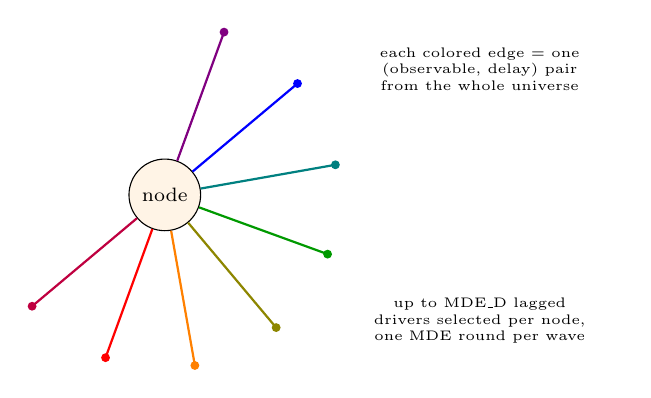
\begin{tikzpicture}[every node/.style={font=\scriptsize}]
  \node[circle, draw, fill=stage2fill, minimum size=9mm] (n) at (0,0) {node};
  \foreach \i/\a/\c in {1/70/violet,2/40/blue,3/10/teal,4/-20/green!60!black,5/-50/olive,6/-80/orange,7/-110/red,8/-140/purple}
    {
      \coordinate (p\i) at ({\a}:2.2cm);
      \draw[\c, thick] (p\i) -- (n);
      \fill[\c] (p\i) circle (1.6pt);
    }
  \node[align=center, font=\tiny, text width=3.4cm] at (4.0,1.6) {each colored edge = one\\(observable, delay) pair\\from the whole universe};
  \node[align=center, font=\tiny, text width=3.4cm] at (4.0,-1.6) {up to MDE\_D lagged\\drivers selected per node,\\one MDE round per wave};
\end{tikzpicture}
\caption{The Stage 2 pass, schematically: one node acquires several lagged coordinates, each independently chosen from every real observable at every candidate delay -- not limited to that node's own Stage-1 neighborhood.}
\label{fig:stage2-schematic}
\end{figure}

\subsection{A lagged pick is its own leaf node}
\label{sec:stage2-leaves}
A lagged pick does not become a delay-annotated edge out of the real observable's node. It becomes a \textbf{node in its own right}, named for the column it is (\texttt{CA1\_3\_tsls::delay-9}) and carrying the graph attributes \texttt{lagged\_of='CA1\_3\_tsls'} and \texttt{lag=-9}. That node has no in-edges, ever. It is a leaf.

Three consequences follow, and the first two are the reason for the design:

\begin{steps}
\item \textbf{A leaf cannot be part of a cycle.} It has in-degree 0 by construction, so no sequence of edges can return to it. Stage 2 therefore needs no acyclicity reasoning at all.
\item \textbf{A lagged copy of an \emph{upstream} observable is legal.} Suppose \texttt{A} already drives \texttt{T}, directly or through a chain. Under the old design, \texttt{A} at delay $-3$ was an edge out of node \texttt{A}, so accepting it would have created a cycle $\texttt{T} \to \dots \to \texttt{A} \to \texttt{T}$ and the pick was rejected. But \texttt{A}'s value three steps ago is not \texttt{A}'s value now: it is a different coordinate, and a legitimate one. The old design was silently discarding valid drivers. As its own leaf, \texttt{A::delay-3} shares no identity with \texttt{A} and the pick stands.
\item \textbf{A leaf is an external input.} \texttt{partition\_network()} (Section~\ref{sec:partition}) classifies every in-degree-0 node as an external input, and gmn feeds those from the recorded data \emph{by node name} -- which is why \texttt{build\_network()} must write one column per leaf into the exported frame, holding that observable shifted by its lag. A leaf whose column is missing has nothing to read. \texttt{tests/test\_lagged\_leaf\_data\_export.py} pins exactly that.
\end{steps}

\begin{figure}[H]
\centering
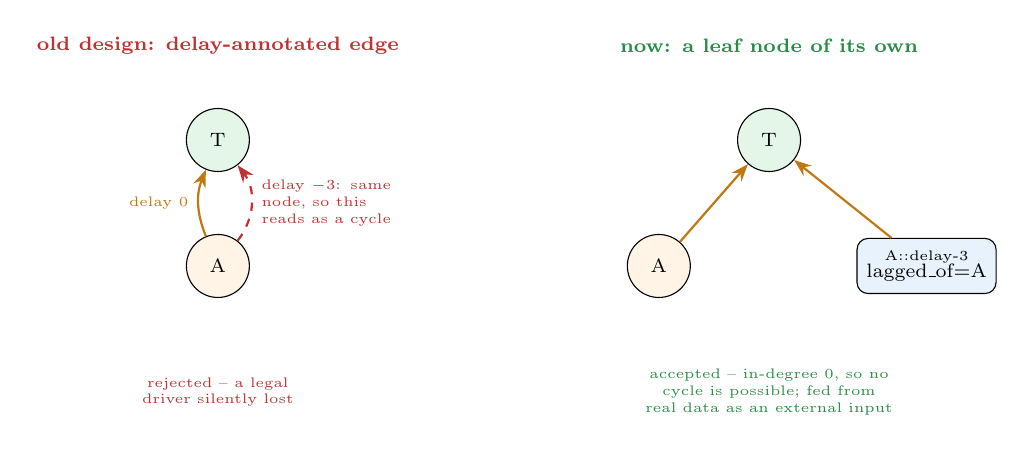
\begin{tikzpicture}[every node/.style={font=\scriptsize}]
  \node[font=\bfseries\scriptsize, badline] at (-3.4,3.0) {old design: delay-annotated edge};
  \node[circle, draw, fill=okfill, minimum size=8mm] (t1) at (-3.4,1.8) {T};
  \node[circle, draw, fill=stage2fill, minimum size=8mm] (a1) at (-3.4,0.2) {A};
  \draw[arrow, stage2line] (a1) to[bend left=22] node[midway, left, font=\tiny] {delay 0} (t1);
  \draw[arrow, badline, dashed] (a1) to[bend right=38] node[midway, right, font=\tiny, text width=1.9cm] {delay $-3$: same node, so this reads as a cycle} (t1);
  \node[font=\tiny, badline, align=center, text width=3.4cm] at (-3.4,-1.4) {rejected -- a legal driver silently lost};

  \node[font=\bfseries\scriptsize, okline] at (3.6,3.0) {now: a leaf node of its own};
  \node[circle, draw, fill=okfill, minimum size=8mm] (t2) at (3.6,1.8) {T};
  \node[circle, draw, fill=stage2fill, minimum size=8mm] (a2) at (2.2,0.2) {A};
  \node[rectangle, draw, rounded corners, fill=stagefill, minimum height=7mm, align=center, font=\tiny] (l2) at (5.6,0.2) {A::delay-3\\\scriptsize lagged\_of=A};
  \draw[arrow, stage2line] (a2) -- (t2);
  \draw[arrow, stage2line] (l2) -- (t2);
  \node[font=\tiny, okline, align=center, text width=4.2cm] at (3.6,-1.4) {accepted -- in-degree 0, so no cycle is possible; fed from real data as an external input};
\end{tikzpicture}
\caption{Why a lagged driver is a leaf node rather than an annotated edge. On the left, \texttt{A} at delay $-3$ is an edge out of node \texttt{A}, so it closes a cycle whenever \texttt{A} is already upstream of \texttt{T} -- and a legal coordinate is thrown away. On the right it is its own node, structurally incapable of forming a cycle.}
\label{fig:stage2-leaves}
\end{figure}

\decisionbox{\texttt{NESTED\_M} governs Stage 1 alone:}{Stage 2 adds only leaves, and a leaf is never expanded, so Stage 2 cannot deepen the network. A node's depth is its distance from the nearest target, and the budget check (\texttt{NESTED\_M == 0 or depth < NESTED\_M}, \texttt{NESTED\_M=0} meaning uncapped) applies to Stage 1's expansion. Stage 1 ends when every live branch's most recent round selected zero drivers, selected only \texttt{NaN}-gain drivers, or hit the depth cap.}

\subsection{Algorithm: \texttt{derive\_lag\_set} -- resolving the candidate delays}
\label{sec:lag-set}
A lag set is a stride and how far back it reaches, so fixing any two of \{stride, count, depth\} determines the third. \texttt{DELAY\_SOURCE} selects which quantity the operator states, and that is the \emph{only} difference between the three paths:
\begin{steps}
\item \texttt{DELAY\_SOURCE='lag\_mode'} (default) pins the \textbf{depth}; the count follows from it. \texttt{LAG\_MODE} sets that depth -- \texttt{'generation\_length\_adjusted'} (default) ties it to \texttt{GENERATE\_LENGTH} (already resolved to a concrete row count by this point, Section~\ref{sec:split}'s pitfall box); \texttt{'every\_lag\_possible'} instead reaches as deep as the MDE library segment $[0,A)$ structurally allows, holding back 50 rows so forward selection still has a usable library once the deepest lag's warm-up \texttt{NaN}s are skipped. The depth is then sampled every \texttt{LAG\_STEP} rows (\texttt{LAG\_DENSITY='strided'}, default) or at every single integer lag (\texttt{'dense'}).
\item \texttt{DELAY\_SOURCE='tau\_count'} pins the \textbf{count}; the depth follows from it. Exactly \texttt{LAG\_COUNT} lags spaced \texttt{LAG\_STEP} apart -- \texttt{LAG\_STEP} playing the role of $\tau$ -- so the deepest lag is $\texttt{LAG\_STEP} \times \texttt{LAG\_COUNT}$. \texttt{LAG\_DENSITY} does not apply here: the stride is always \texttt{LAG\_STEP}, and \texttt{LAG\_STEP=1} therefore gives consecutive lags.
\item \texttt{DELAY\_SOURCE='explicit'} pins \textbf{every value}: the hand-picked \texttt{DELAY\_SET} list, with any \texttt{0} entry stripped.
\end{steps}
All three return the same shape -- a descending list of negative integers, never containing \texttt{0}; the \texttt{0} is reintroduced only when the set is reused as a node's \texttt{self\_delay\_set} (Section~\ref{sec:self-delay}). An unrecognized \texttt{DELAY\_SOURCE} raises rather than falling through to the auto path, so a typo cannot quietly run a different algorithm than the one asked for.

Only the \emph{resolved list} reaches the cache fingerprint (\texttt{build\_network\_fingerprint}'s \texttt{delay\_set} field, Section~\ref{sec:reuse}), never which source produced it. Restating an auto-derived set as the equivalent \texttt{tau\_count} therefore reuses cached MDE work, while changing \texttt{LAG\_COUNT} correctly invalidates it -- both pinned by \texttt{tests/test\_lag\_set\_sources.py}.

\decisionbox{Why \texttt{tau\_count} exists: the number of lags is a compute budget, and under \texttt{lag\_mode} nobody states it:}{Stage 2 offers MDE one candidate column per (real observable $\times$ lag), and Stage 2 is where essentially all of a run's wall-clock goes (Section~\ref{sec:history-stage1-cost}: single Stage 2 nodes have taken 36\,h). The count is therefore the bill. Under \texttt{'lag\_mode'} it is \emph{derived}, and derived from a knob chosen for an unrelated purpose: \texttt{'generation\_length\_adjusted'} ties it to \texttt{GENERATE\_LENGTH}, which means how many steps \texttt{Generate()} free-runs for. Those two quantities have no reason to agree. The shipped \texttt{tsls-mde-gmn.sbatch} (\texttt{GENERATE\_LENGTH=400}, \texttt{LAG\_STEP=4}) resolves to 100 lags per observable, and leaving \texttt{GENERATE\_LENGTH} at its \texttt{0} default resolved to roughly 830 -- Section~\ref{sec:history-generate-length} is that trap being caught by hand during review, and the GPU fork's sizing note records \texttt{GENERATE\_LENGTH} being held at 400 \emph{deliberately}, against an otherwise uniform halving, purely to keep the lag count down. \texttt{tau\_count} lets the budget be stated directly, so narrowing Stage 2 no longer shortens the \texttt{Generate()} run as a side effect.}
\pitfallbox{Column naming and delay-expansion are pure DataFrame mechanics, unaffected by TSLS:}{\texttt{DELAY\_MARKER}/\texttt{\_delayed\_column\_name}/\texttt{\_parse\_delayed\_column\_name}/\texttt{observable\_and\_delay}/\texttt{expand\_delay\_columns} operate on column \emph{names} and row-shifted values, with no dependency on what a column represents -- reused unchanged against TSLS's own \texttt{\_tsls}-suffixed names (e.g.\ \texttt{CA1\_2\_tsls::delay-9}, confirmed in real output, Section~\ref{sec:outputs}). \texttt{expand\_delay\_columns} still produces leading \texttt{NaN} warm-up rows for every shifted column -- the same warm-up convention \texttt{run\_mde\_for\_target}'s leakage guard (Section~\ref{sec:leakage-guard}) already skips past, and the same convention whose omission caused the PCA history bug (Section~\ref{sec:history-pca}).}

\linknote{Both phases mutate the same \texttt{MultiDiGraph} in place. By the time \texttt{build\_nested\_mde\_network()} returns, that graph -- not an interaction matrix -- \emph{is} the network. Before it can simulate, one more question has to be settled: does every node in this graph, including a zero-driver leaf, deserve to be treated as something nested-MDE actually \emph{found}? Section~\ref{sec:partition} (R14) answers that; Section~\ref{sec:smap} is the patch that lets gmn simulate whatever the answer leaves behind.}

\newpage
% =====================================================================
\section{Leaf Partitioning: External Inputs vs.\ Simulated Nodes}
\label{sec:partition}
% =====================================================================

\subsection{The problem: a zero-driver leaf used to simulate itself out of nothing}
Before this change, every node the graph contained -- a real interior node with discovered drivers, or a leaf nested-MDE selected but which itself has zero drivers of its own -- got the identical treatment: an unconditional self-history embedding (Section~\ref{sec:self-delay}), fed through gmn's own SMap machinery every simulated step. A zero-driver leaf therefore predicted its own future from nothing but its own past, never touching real data again after the initial seed -- exactly what let Section~\ref{sec:overview}'s "runs freely... without ever seeing the real behavior again" claim hold for \emph{every} node, leaf or not. Review found this overstates what nested-MDE actually discovered: a zero-driver node is not something Stage 1/2 found as a network member, so simulating it as if it were one is misleading, not merely redundant.

\subsection{Algorithm: \texttt{partition\_network}}
\label{sec:partition-algo}
\begin{steps}
\item Classify every node by in-degree: \textbf{interior} (\texttt{in\_degree} $\ge 1$ -- nested-MDE found at least one driver for it) or \textbf{external input} (\texttt{in\_degree} $= 0$). Every Stage 2 leaf (Section~\ref{sec:stage2-leaves}) lands in the second class by construction, which is the intended reading: a lagged coordinate is input the network does not explain.
\item \textbf{Raise immediately if a \emph{target} itself has zero drivers} (Run A's own \texttt{head\_position\_y}, Section~\ref{sec:outputs}, is exactly this case), regardless of \texttt{EXTERNAL\_INPUT\_MODE}: classifying a target as external would feed its own real recorded values back in as its "simulation" (Section~\ref{sec:partition-mode} below) and then score fidelity against those same real values -- circular, spuriously perfect, for precisely the case that most needs flagging as a failure, not celebrating as a success.
\item Store the classification explicitly on \texttt{graph.graph} (\texttt{interior\_nodes}/\texttt{external\_inputs}/\texttt{external\_input\_mode}) rather than leaving it implicit in edge counts, so every later consumer reads one authoritative classification instead of re-deriving it.
\item \texttt{report\_partition()}: prints the partition to the run log and writes \texttt{partition\_\{network\_id\}.csv} (node, role, feeds, delay) to \texttt{results\_dir}.
\end{steps}

\begin{figure}[h]
\centering
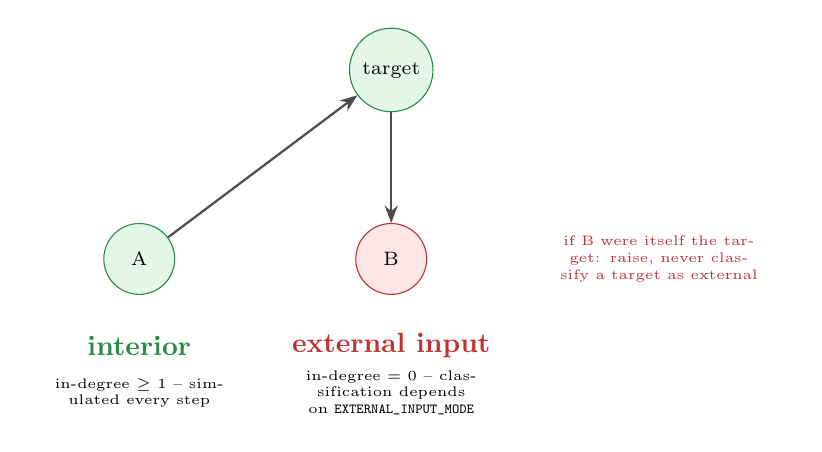
\begin{tikzpicture}[every node/.style={font=\scriptsize}]
  \node[circle, draw=okline, fill=okfill, minimum size=9mm] (t) at (3.2,2.4) {target};
  \node[circle, draw=okline, fill=okfill, minimum size=9mm] (a) at (0,0) {A};
  \node[circle, draw=badline, fill=badfill, minimum size=9mm] (b) at (3.2,0) {B};
  \draw[arrow] (a) -- (t);
  \draw[arrow] (t) -- (b);
  \node[font=\bfseries, okline] at (0,-1.1) {interior};
  \node[font=\tiny, align=center, text width=2.6cm] at (0,-1.7) {in-degree $\ge$ 1 -- simulated every step};
  \node[font=\bfseries, badline] at (3.2,-1.1) {external input};
  \node[font=\tiny, align=center, text width=2.8cm] at (3.2,-1.7) {in-degree = 0 -- classification depends on \texttt{EXTERNAL\_INPUT\_MODE}};
  \node[font=\tiny, align=center, text width=3.2cm, badline] at (6.6,0) {if B were itself the target: raise, never classify a target as external};
\end{tikzpicture}
\caption{\texttt{partition\_network()}'s classification: A has a real driver, so it is interior; B has none, so it is an external input -- unless B is itself one of \texttt{TARGETS}, in which case \texttt{partition\_network} raises rather than silently accepting a self-scoring target.}
\label{fig:partition}
\end{figure}

\subsection{\texttt{EXTERNAL\_INPUT\_MODE}: what an external input actually does during simulation}
\label{sec:partition-mode}
\begin{steps}
\item \texttt{'real\_data'} (\textbf{the default}): an external input is treated as a genuine exogenous input in the standard control-theory sense -- \texttt{Generate()} returns the real recorded value at the current row instead of running SMap at all; \texttt{Forecast()} returns the real series as a trivial passthrough. It never reaches \texttt{\_embedding\_spec\_for()} (Section~\ref{sec:smap}) in the first place -- short-circuited earlier, inside the \texttt{gmn.Node} monkeypatches themselves.
\item \texttt{'self\_simulate'}: keeps the pre-R14 behavior -- an external input still runs SMap on its own unconditional self-history, exactly like before this change existed.
\item \texttt{\_simulated\_nodes(graph)}: the set of nodes that actually run gmn's SMap machinery (every interior node, always; external inputs only under \texttt{'self\_simulate'}) -- used by \texttt{run\_theta\_search()} so a \texttt{'real\_data'}-mode external input (no embedding, nothing to retune) is correctly excluded from theta retuning rather than silently retuned against meaningless input.
\end{steps}
\decisionbox{Why a toggle, not one fixed behavior:}{Whether an external input should be fed real data or left self-simulating is a genuine modeling choice, not something the codebase should decide unilaterally -- \texttt{'real\_data'} is the more standard reading of "external input," but a reviewer who specifically wants to see how the pre-R14 architecture behaves (or wants every node genuinely free-running, no real data reinjected anywhere past the initial seed) can still get that with \texttt{'self\_simulate'}.}
\pitfallbox{Bug found while testing this, not anticipated by the original task text:}{\texttt{\_generalized\_node\_generate()}/\texttt{\_generalized\_node\_forecast()}'s own SMap call used \texttt{columns=df.columns[1:-1]} -- dropping \texttt{time} (first) \emph{and} the embedding spec's own last entry. Before this change this was harmless (\texttt{self\_delay\_set} always padded a node with several self-lags, so losing one rarely mattered); after it, a node's spec \emph{is} its discovered drivers, so a single-driver interior node lost its \emph{only} predictor column entirely -- a hard \texttt{pyEDM} crash (\texttt{RuntimeError: Validate() SMap: columns required.}), and a 2+-driver node silently lost its last one. Fixed to \texttt{columns=df.columns[1:]} (drop only \texttt{time}) in both functions, both pipelines -- a general fix, not specific to this task, but found and landed together with it since this change is what turned a masked quirk into a real risk.}

\subsection{Correction: the self-history "anchor" cannot be removed entirely}
The original instruction behind this feature asked for a node's embedding to be built "only from drivers discovered by nested-MDE," with \texttt{self\_delay\_set} (Section~\ref{sec:self-delay}) removed outright. Confirmed directly against \texttt{pyEDM}: this breaks every interior node, not just an edge case -- \texttt{target=node\_name+\texttt{'(t-0)'}} is a hard \texttt{pyEDM} requirement, and no in-edge can ever supply it (self-loops are excluded by \texttt{\_accept\_mde\_result\_edges()}'s own guard). The design instead keeps a node's own delay=0 value as an unconditional \textbf{anchor} coordinate -- standard generalized-embedding practice besides, since a variable's own present value is conventionally one of its own state-space coordinates -- and removes only the \emph{deeper} self-lags the original instruction actually objected to. \texttt{\_embedding\_spec\_for()} is therefore simply \texttt{[(node\_name, 0)] + in\_edges} for every node that reaches it (every interior node, always; an external input only under \texttt{'self\_simulate'}) -- no separate interior/external branching inside the function itself, since the mode-driven behavior lives entirely in the \texttt{Generate()}/\texttt{Forecast()}/\texttt{\_\_init\_\_} short-circuits above.

\subsection{\texttt{plot\_3d\_network()}: a new diagnostic}
$x$-$y$ plane is a layout of the real-observable (delay=0) backbone; $z$-axis is one vertical stick per delay$\ne$0 driver, rising to $|{\rm delay}|$ at the driven node's $(x,y)$; external inputs are drawn as a distinct marker shape (triangle vs.\ circle) from interior nodes, independent of target coloring. Produced alongside the existing \texttt{draw\_colored\_network()} for every \texttt{MODE='MDE-GMN'} run.

\linknote{Every node the graph contains is now classified. Section~\ref{sec:smap} covers how an interior node's own (anchor + in-edges) spec becomes an actual non-uniform embedding gmn can simulate.}

\newpage
% =====================================================================
\section{proper\_mde: The Selection Engine Both Stages Share}
\label{sec:mde-engine}
% =====================================================================
Every MDE call in both stages (and \texttt{main()}'s own depth-0 seed) routes through \texttt{run\_mde\_for\_target()}, this pipeline's own wrapper around \texttt{cleaned\_helper\_functions.proper\_mde} -- a from-scratch, KD-tree-based re-implementation of the same greedy forward-selection algorithm the sibling pipeline's third-party \texttt{dimx.MDE} runs, built specifically so its internal scoring is \emph{pluggable}.

\subsection{Algorithm: \texttt{proper\_mde} -- the ranking stage}
\label{sec:mde-ranking}
\textit{(cleaned\_helper\_functions.py; this and the next subsection together are "one dimension" of the outer \texttt{for d in range(1, D+1)} loop)}
\begin{steps}
\item For dimension $d$, form one candidate column list per not-yet-selected column: each candidate is tried \emph{prepended} to whatever has already been selected.
\item For every such list, run a genuine multivariate Simplex prediction of the target using that exact column list as a ready-made embedding (\texttt{embedded=True} -- each selected column is one raw coordinate, no further delay-lagging), scored with \texttt{target\_metric} (\texttt{TARGET\_METRIC}, always \texttt{'correlation'} -- the value being predicted is always a target, Section~\ref{sec:target-metric}).
\item Sort candidates best-first (\texttt{NaN} scores always sort last).
\item Drop every candidate failing \texttt{crossMapRhoMin}. If nothing survives, skip to dimension $d{+}1$ without adding anything.
\end{steps}

\subsection{Algorithm: \texttt{proper\_mde} -- the CCM causality gate}
\label{sec:mde-ccm-gate}
\begin{steps}
\item Walk the ranked, threshold-surviving candidates \textbf{best-first}: accept the \emph{first} candidate that also passes a causality check, not necessarily the single best-ranked one.
\item For each candidate: resolve its embedding dimension (a caller-supplied static $E$ here); reject if that embedding's own skill fails \texttt{embedDimRhoMin}; run the CCM convergence test (Section~\ref{sec:ccm}) using \texttt{metric} (\texttt{METRIC}, \texttt{'f1'} by default -- this candidate is a TSLS series, Section~\ref{sec:target-metric}); accept and stop walking the moment one passes.
\item If the whole ranked list is exhausted with nothing passing, terminate the entire search early, not just this dimension.
\end{steps}

\begin{figure}[H]
\centering
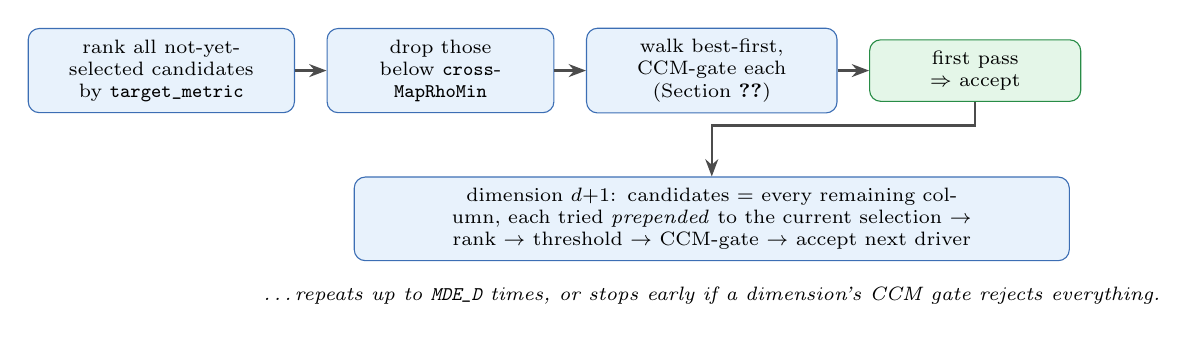
\begin{tikzpicture}[node distance=4mm, every node/.style={font=\scriptsize}]
  \node[smallbox, text width=3.1cm] (cands) {rank all not-yet-\\selected candidates\\by \texttt{target\_metric}};
  \node[smallbox, text width=2.6cm, right=of cands] (thresh) {drop those\\below \texttt{cross}-\\\texttt{MapRhoMin}};
  \node[smallbox, text width=2.9cm, right=of thresh] (ccm) {walk best-first,\\CCM-gate each\\(Section~\ref{sec:ccm})};
  \node[smallbox, text width=2.4cm, right=of ccm, fill=okfill, draw=okline] (accept) {first pass\\$\Rightarrow$ accept};
  \draw[arrow] (cands) -- (thresh);
  \draw[arrow] (thresh) -- (ccm);
  \draw[arrow] (ccm) -- (accept);
  \node[smallbox, text width=8.8cm, below=8mm of ccm, fill=stagefill] (next) {dimension $d{+}1$: candidates = every remaining column, each tried \emph{prepended} to the current selection $\to$ rank $\to$ threshold $\to$ CCM-gate $\to$ accept next driver};
  \draw[arrow] (accept.south) -- ++(0,-3mm) -| (next.north);
  \node[below=2mm of next, font=\scriptsize\itshape] {\ldots repeats up to \texttt{MDE\_D} times, or stops early if a dimension's CCM gate rejects everything.};
\end{tikzpicture}
\caption{One dimension of \texttt{proper\_mde}'s forward selection: rank first (cheap), then causality-gate only the survivors, accepting the first ranked candidate that also passes CCM.}
\label{fig:mde-flow}
\end{figure}

\subsection{The exclusion-radius parameter}
\label{sec:exclusion-radius}
The classic Theiler-window guideline is $\texttt{exclusionRadius} \ge E \times \tau$ -- but this pipeline's embeddings are generalized (Section~\ref{sec:stage2}), so $E$ and $\tau$ are confounded rather than fixed scalars. The sibling pipeline addresses this with a dynamic, per-internal-call \texttt{'auto'} mode that intercepts \texttt{dimx.Run}'s own staged sequence of internal calls and recomputes the radius fresh at each one (sibling document, Section~\ref{sec:sibling}'s own cross-reference). \texttt{proper\_mde} has no equivalent staging to intercept: it is a single opaque call per dimension, taking one \texttt{exclusionRadius} \emph{floor} value for its whole internal search. \texttt{EXCLUSION\_RADIUS} the config knob is therefore still a \textbf{plain static integer, no \texttt{'auto'} choice} -- full parity with the sibling's own per-call auto mode is still not achievable, given \texttt{proper\_mde}'s single-call architecture.

\subsection{R21: a dynamic radius \emph{within} \texttt{proper\_mde}, orthogonal to the static floor above}
\label{sec:exclusion-radius-dynamic}
A narrower, genuinely dynamic mechanism was added on top of the static floor -- not a replacement for it, and not the sibling's own per-call \texttt{'auto'} mode, but closing a real, separate gap review found: \texttt{proper\_mde} has no built-in concept of "delay" attached to a column name at all (delay is purely a naming convention, \texttt{DELAY\_MARKER}/\texttt{observable\_and\_delay()}, that lives in \texttt{tsls-mde-gmn.py}, not in \texttt{cleaned\_helper\_functions.py}) -- yet a real candidate pool routinely contains delay-suffixed synthetic names at \emph{both} Stage 1 and Stage 2 (confirmed via real selections: \texttt{CA1\_1\_tsls::delay-25} alongside \texttt{CA1\_1\_tsls} itself in the same \texttt{MDEcolumns} list), so a static \texttt{exclusionRadius} could under-exclude once a deeply-lagged column had already been selected earlier in the same forward-selection search.
\begin{steps}
\item \texttt{proper\_mde()} gained a new \texttt{column\_delay=None} parameter (a caller-supplied \texttt{\{column: delay\}} lookup; \texttt{None} is an exact no-op, so every existing caller that doesn't opt in is unaffected).
\item At each forward-selection dimension $d$, before that dimension's E-select and CCM-gate calls: $\texttt{exclusionRadius}_d = \max(\texttt{exclusionRadius}, \max_{c \,\in\, \mathrm{selected}} |\texttt{column\_delay}(c)|)$ -- the deepest delay among columns already selected in \emph{earlier} dimensions of this same call (never the current dimension's own not-yet-accepted candidate). Logged once per dimension (\texttt{\{d\}-D exclusionRadius=... (floor=..., deepest\_selected\_lag=...)}), reaching every real run's log automatically since \texttt{run\_mde\_for\_target()} already calls \texttt{proper\_mde} with \texttt{verbose=True}.
\item \texttt{run\_mde\_for\_target()} builds \texttt{column\_delay} from \texttt{observable\_and\_delay(c, raw\_columns)} for every candidate column and passes it through at both of Stage 1/Stage 2's own call sites (the two places a delay-suffixed candidate pool genuinely reaches \texttt{proper\_mde}); \texttt{main()}'s own depth-0 seed leaves it at \texttt{None} (its own candidate pool is always real-only).
\end{steps}
\decisionbox{Deliberately confined to the ranking/CCM-gate calls, not the ranking metric itself:}{The ranking stage's own \texttt{\_simplex\_metric} call has never accepted an \texttt{exclusionRadius} at all -- a separate, pre-existing limitation this change doesn't address -- and \texttt{multi\_proper\_mde} (a different function entirely) is untouched, left for a future unification of the two call paths.}
\pitfallbox{Confirmed genuinely active, not a no-op that happens to match by construction:}{On real data, selections came out identical with and without \texttt{column\_delay} in one tested configuration -- but at the dimension where the radius genuinely differed (6 dynamic vs.\ 0 static), several candidates' own embedding-dimension and CCM-slope numbers measurably differed between the two runs; none of those differences happened to flip which candidate was \emph{first} to pass the gate in this particular case, so the final selection matched by coincidence, not because the mechanism was inert.}

\newpage
% =====================================================================
\section{Per-Node Ranking-Window Sizing: \texttt{MIN\_PRED\_EVENTS} and \texttt{MAX\_WINDOW\_ROWS}}
\label{sec:window-sizing}
% =====================================================================

\subsection{How this was found: a metric-routing bug exposed a deeper calibration problem}
\label{sec:metric-routing-bug}
Review tracing a verbose log line found that Stage 1/Stage 2's own \texttt{executor.submit(run\_mde\_for\_target, ...)} call sites passed the closed-over \texttt{target\_metric} \emph{positionally, unconditionally, for every node} -- never resolved per-node via \texttt{\_metric\_for()} (Section~\ref{sec:target-metric}). That split is correct exactly once: \texttt{main()}'s own depth-0 seed, where \texttt{target} is always a real behavioral column. At depth $\ge 1$ (Stage 1's own recursion; all of Stage 2), the node being ranked is virtually always a \emph{neuron}, which should score via \texttt{'f1'}, not \texttt{'correlation'} -- a rule this call site never consulted. \textbf{Net effect: every discovered neuron driver's own ranking-stage acceptance had been scored via Pearson correlation on a TSLS sawtooth, not the TSLS-aware event metric \texttt{\_metric\_for()} says it should use}, for this whole redesign and presumably before it. Fixed by replacing the raw positional argument with \texttt{\_metric\_for(node, targets, metric, target\_metric)} at both call sites -- a one-line fix per site, but one that could not simply be merged without first checking what it would do to real selections.

\textbf{The required recalibration check found the fix was not safe to land as-is.} At the old fixed \texttt{CCM\_WINDOW\_ROWS=800} window, the ranking stage's own derived prediction slice was 141 rows -- and \texttt{f1} came back \textbf{exactly 0.0000 for every one of 44 real candidates, for all three real neuron targets tested.} Counting actual TSLS reset events in that 141-row slice directly: 0, 1, and 0 events respectively -- with 0--1 true events, \texttt{f1} is structurally degenerate regardless of prediction quality; the window was simply too event-sparse. Correlation, scored over the identical window, showed a healthy, informative spread (8--18 of 44 candidates passing threshold) -- this was not a generically-too-small window, it was specifically inadequate for an event-counting metric.

\subsection{Root cause: firing-rate heterogeneity, not just window size}
Counting real TSLS reset events for all 45 real channels at this scale: \textbf{21/45 (47\%) had zero events in the 141-row prediction window}; several had zero events in the entire 800-row frame. Rows needed to reach 20 events (this investigation's own working definition of "enough for \texttt{f1} to be trustworthy" -- below 20 true events, a single miss or false positive swings the score by $\ge 5$ percentage points): minimum 98, median 1{,}600, and several channels never reach it within any window this dataset's own leakage boundary allows. \textbf{A single fixed window cannot serve both ends of this distribution} -- a bigger single number only helps the faster-firing quartile; the slowest channels need thousands of rows or effectively can't reach a fixed target at all. This is why the fix became a redesign of the ranking window itself, not just the metric-routing one-liner.

\subsection{Design evolution: two abandoned iterations before the final design}
\begin{figure}[H]
\centering
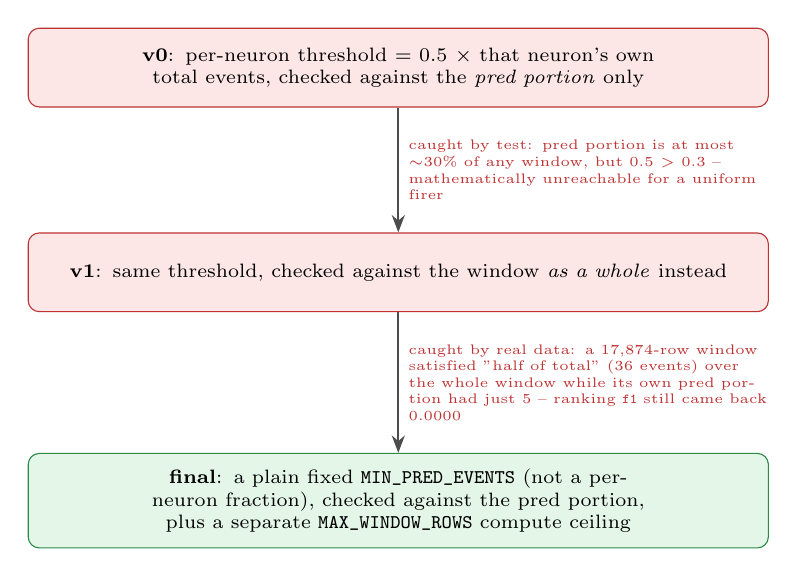
\begin{tikzpicture}[every node/.style={font=\scriptsize}, node distance=6mm]
  \node[rectangle, draw=badline, fill=badfill, rounded corners, minimum width=9.4cm, text width=9.0cm, minimum height=1.0cm, align=center] (v0) at (0,4.6) {\textbf{v0}: per-neuron threshold = 0.5 $\times$ that neuron's own total events, checked against the \emph{pred portion} only};
  \node[rectangle, draw=badline, fill=badfill, rounded corners, minimum width=9.4cm, text width=9.0cm, minimum height=1.0cm, align=center] (v1) at (0,2.0) {\textbf{v1}: same threshold, checked against the window \emph{as a whole} instead};
  \node[rectangle, draw=okline, fill=okfill, rounded corners, minimum width=9.4cm, text width=9.0cm, minimum height=1.2cm, align=center] (v2) at (0,-0.9) {\textbf{final}: a plain fixed \texttt{MIN\_PRED\_EVENTS} (not a per-neuron fraction), checked against the pred portion, plus a separate \texttt{MAX\_WINDOW\_ROWS} compute ceiling};
  \draw[arrow] (v0) -- (v1) node[midway, right, badline, align=left, text width=4.6cm, font=\tiny] {caught by test: pred portion is at most $\sim$30\% of any window, but 0.5 $>$ 0.3 -- mathematically unreachable for a uniform firer};
  \draw[arrow] (v1) -- (v2) node[midway, right, badline, align=left, text width=4.6cm, font=\tiny] {caught by real data: a 17,874-row window satisfied "half of total" (36 events) over the whole window while its own pred portion had just 5 -- ranking \texttt{f1} still came back 0.0000};
\end{tikzpicture}
\caption{Both intermediate designs were caught before shipping -- v0 by a unit test, v1 by real end-to-end verification -- not by inspection. The underlying diagnosis: a \emph{fraction of a neuron's own total events} is the wrong kind of quantity here regardless of which part of the window it's checked against; it makes a busy neuron face a stricter test than a quiet one for no stated reason, and gives the sparsest (least reliable) neurons the \emph{weakest} requirement. "How many matched events does \texttt{f1} need before it's signal rather than noise" is a property of the metric, not of the neuron.}
\label{fig:window-sizing-evolution}
\end{figure}

\subsection{Final design: \texttt{MIN\_PRED\_EVENTS} + \texttt{MAX\_WINDOW\_ROWS}}
\label{sec:window-sizing-final}
\begin{steps}
\item \textbf{Behavioral targets (depth 0)} keep the separate, fixed \texttt{TARGET\_RANKING\_WINDOW\_ROWS=1000} window -- no event-count concept applies to a continuous trace.
\item \textbf{Every depth $\ge 1$ (neuron) node}: \texttt{\_resolve\_target\_ranking\_window()} grows a candidate window $W$ (rows); the \textbf{pred portion} is $W$'s own last $(1{-}\texttt{lib\_ratio})$ fraction -- the identical split \texttt{\_ccm\_window()} will later carve out of this same $W$ for the CCM gate, so the two agree by construction. Count the target's real reset events in that row range (by \emph{rows}, never by events, and strictly within $[0,B)$ -- counting into held-out rows would be the same class of leakage the $B$ boundary exists to prevent) and stop at the smallest $W$ where the count is $\ge$ \texttt{MIN\_PRED\_EVENTS} (\textbf{default 20}, a plain fixed integer -- not a fraction of anything neuron-specific).
\item \texttt{MAX\_WINDOW\_ROWS} (\textbf{default 30{,}000}) is a separate compute ceiling, not itself calibrated: if a node can't reach \texttt{MIN\_PRED\_EVENTS} within $\min(\texttt{MAX\_WINDOW\_ROWS}, \mathrm{len(usable\_df)})$, it is \textbf{skipped -- logged with the reason and the shortfall} -- rather than scored on too few events. \texttt{MIN\_PRED\_EVENTS} is the statistical floor; \texttt{MAX\_WINDOW\_ROWS} is the compute ceiling; the two express one thing each.
\end{steps}

\begin{figure}[h]
\centering
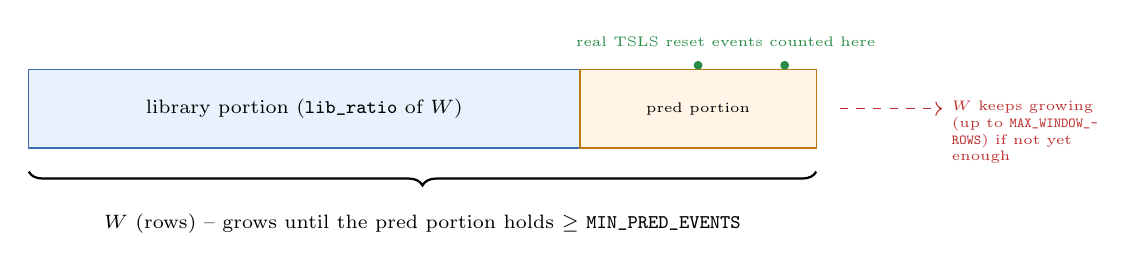
\begin{tikzpicture}[scale=1.0, every node/.style={font=\scriptsize}]
  \draw[fill=stagefill, draw=stageline] (0,0) rectangle (7.0,1);
  \node[align=center] at (3.5,0.5) {library portion (\texttt{lib\_ratio} of $W$)};
  \draw[fill=stage2fill, draw=stage2line] (7.0,0) rectangle (10.0,1);
  \node[align=center, font=\tiny] at (8.5,0.5) {pred portion};
  \foreach \x/\e in {7.4/0,8.5/1,9.1/0,9.6/1} {
    \ifnum\e=1 \fill[okline] (\x,1.05) circle (1.6pt); \fi
  }
  \node[font=\tiny, okline] at (8.85,1.35) {real TSLS reset events counted here};
  \draw[decorate, decoration={brace, amplitude=5pt}, thick] (10.0,-0.3) -- (0,-0.3);
  \node[below=6pt] at (5.0,-0.5) {$W$ (rows) -- grows until the pred portion holds $\ge$ \texttt{MIN\_PRED\_EVENTS}};
  \draw[->, dashed, badline] (10.3,0.5) -- (11.6,0.5);
  \node[right, font=\tiny, badline, align=left, text width=2.0cm] at (11.6,0.2) {$W$ keeps growing (up to \texttt{MAX\_WINDOW\_ROWS}) if not yet enough};
\end{tikzpicture}
\caption{\texttt{\_resolve\_target\_ranking\_window()}: only the pred portion's own events count toward \texttt{MIN\_PRED\_EVENTS} -- the same portion \texttt{f1}-scoring will actually read at the ranking stage.}
\label{fig:window-growth}
\end{figure}

\pitfallbox{Non-monotonicity, found while writing the test, not by inspection:}{The pred portion's own event count is \emph{not} guaranteed to increase monotonically as $W$ grows: both of its edges only ever move forward, so its width never shrinks, but in a single step an event row can age out of the advancing left edge before a new event row enters at the right, so the count can dip locally. Consequence: on a failure (node skipped), the reported best-achieved count must be the \emph{maximum seen at any window size tried}, not just the count at the cap -- the first implementation used the naive "count at the cap" and was corrected before shipping, once a dedicated test independently re-derived the true best-achievable count by brute force and caught the mismatch.}

\subsection{\texttt{MIN\_PRED\_EVENTS=20}: a cost/reachability choice, not a discovered threshold}
Calibrated by adding synthetic Gaussian noise (5\% of a real TSLS slice's own std, 200 draws) and measuring how \texttt{f1}'s own noise floor (std across draws) falls as the target pred-event count grows, pooled across 15 real channels stratified by firing-rate tercile:

\begin{figure}[h]
\centering
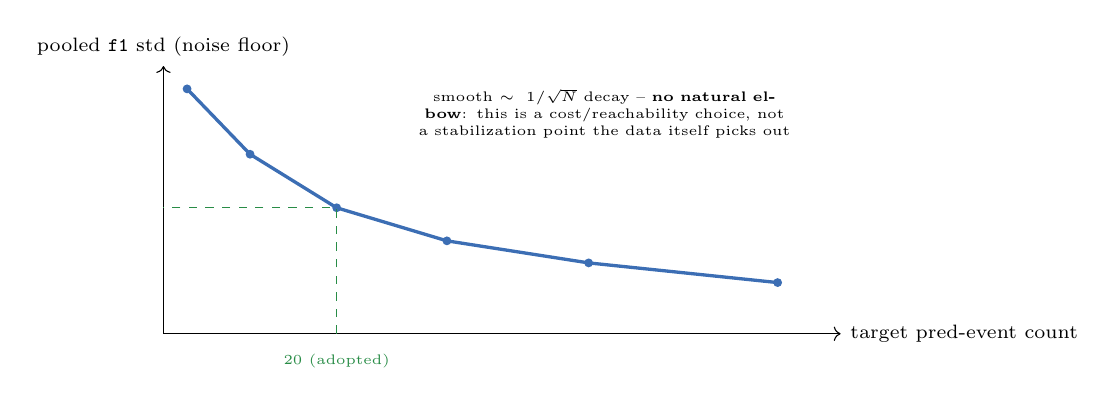
\begin{tikzpicture}[scale=1.0, every node/.style={font=\scriptsize}]
  \draw[->] (0,0) -- (8.6,0) node[right] {target pred-event count};
  \draw[->] (0,0) -- (0,3.4) node[above] {pooled \texttt{f1} std (noise floor)};
  \draw[stageline, very thick]
    plot coordinates {(0.3,3.11) (1.1,2.28) (2.2,1.60) (3.6,1.18) (5.4,0.90) (7.8,0.65)};
  \foreach \x/\y/\lab in {0.3/3.11/5, 1.1/2.28/10, 2.2/1.60/20, 3.6/1.18/40, 5.4/0.90/80, 7.8/0.65/160}
    \fill[stageline] (\x,\y) circle (1.6pt);
  \draw[dashed, okline] (2.2,0) -- (2.2,1.60) -- (0,1.60);
  \node[okline, font=\tiny] at (2.2,-0.35) {20 (adopted)};
  \node[font=\tiny, align=center, text width=5.4cm] at (5.6,2.8) {smooth $\sim 1/\sqrt{N}$ decay -- \textbf{no natural elbow}: this is a cost/reachability choice, not a stabilization point the data itself picks out};
\end{tikzpicture}
\caption{Doubling the target pred-event count roughly halves \texttt{f1}'s own noise floor at every step from 10 to 160 -- a smooth curve with nothing that looks like "enough." At 20, std $\approx 0.07$ is still $\sim$3$\times$ smaller than \texttt{CROSS\_MAP\_RHO\_MIN}'s own 0.2 default.}
\label{fig:min-pred-events-calibration}
\end{figure}

Real-data reachability at \texttt{REGION\_CHANNEL\_CAP=15} (45 channels) directly informed the choice: at 20, only 3/45 channels are unreachable (window\_rows spanning 407--26{,}748 for the rest); at 40, 8/45; at 80, nearly half (20/45). 40 and 80 buy modestly less noise at a steep cost in both unreachable channels and window length -- diminishing returns, not a clear win. \texttt{MAX\_WINDOW\_ROWS=30{,}000} is set comfortably above the largest reachable requirement observed (26{,}748) and safely below this dataset's own leakage boundary ($B \approx 38{,}067$ at this configuration).

\subsection{CCM-gate candidate-side event sufficiency: measured, then a diagnostic, not a skip}
\texttt{MIN\_PRED\_EVENTS} only guarantees the \emph{target}'s own events in the ranking window's pred slice -- it says nothing about whether a given \emph{candidate} has enough of its own events in the CCM gate's own frame (which has no lib/pred split at all). \textbf{Verified, not assumed, that this never causes a false pass}: with 0 real candidate events, \texttt{f1} is identically 0 for every sample/library-size cell (recall is $0/0$), so the fitted convergence slope is exactly 0, never above threshold; simulated under a genuine null (independent target/candidate, no causal link) at candidate-event counts 0 through 19, \textbf{0/360 false passes} observed across every count tested. \textbf{But starvation itself is real, not negligible}: at the median resolved window ($\sim$3{,}600 rows), 6/45 real channels (13\%) would themselves be starved if they appeared as a candidate there; at the larger windows slower targets require ($\ge$10{,}400 rows), 0/45 are starved -- concentrated exactly where fast-firing, small-window targets meet their slower candidate-partners.
\decisionbox{Decision: rely on the existing convergence-slope gate (already proven safe above), add one diagnostic, no new control flow:}{Both \texttt{proper\_mde} and \texttt{multi\_proper\_mde}'s own CCM-gate loops now log the candidate's own event count in the frame, alongside the fitted slope, whenever \texttt{ccmMetric == 'f1'}. The real cost of doing nothing was never wrong selections (0/360 proves that) -- it was that an event-starved candidate and a genuinely non-causal one were previously indistinguishable in the output, both recorded simply as "failed the gate." The log line makes them separable after the fact, at no runtime cost. An explicit candidate-side skip remains available if a future pass finds this matters more than the 13\%/0\% split suggests.}

\subsection{\texttt{CCM\_LIB\_SIZES\_ROWS}: decoupling the CCM gate's own library-size sweep}
\texttt{CCM\_WINDOW\_ROWS}/\texttt{CCM\_LIB\_SIZE\_PCTS} (Section~\ref{sec:calibration}) previously bounded two different things through one shared, fixed-size frame: the ranking-stage window above (now per-node and node-specific, not fixed) and the CCM gate's own \texttt{libSizes} sweep (a percentage of that same, now-variable, window). \texttt{proper\_mde}/\texttt{multi\_proper\_mde} gained a \texttt{libSizes=None} parameter that, given an explicit list, bypasses the percentage-of-$N$ computation entirely; \texttt{run\_mde\_for\_target()}/\texttt{run\_multi\_mde\_for\_targets()} now pass \texttt{CCM\_LIB\_SIZES\_ROWS} -- \textbf{absolute row counts, default $(16, 24, 40, 64, 160, 400, 800)$} (R9/R17's own already-calibrated percentage grid, evaluated once at the old 800-row frame, plus one additional point for plateau visibility at larger scales) -- instead. \textbf{Re-validated on real data} that these same absolute values still show the identical rising-then-plateauing convergence shape at an 8{,}000-row frame, not only the 800-row scale they were originally picked at -- confirming the shape is a property of the absolute library size, not its ratio to the surrounding frame.
\pitfallbox{\texttt{CCM\_WINDOW\_ROWS}/\texttt{CCM\_LIB\_SIZE\_PCTS} are now \texttt{MODE='GMN'}-only:}{\texttt{MODE='MDE-GMN'} (this pipeline's default) no longer uses either -- the CCM pre-filter (Section~\ref{sec:ccm-prefilter}) and \texttt{proper\_mde}'s own gate now use the per-node ranking window and \texttt{CCM\_LIB\_SIZES\_ROWS} respectively. Only \texttt{MODE='GMN'}'s own interaction matrix (\texttt{build\_interaction\_matrix()}, Section~\ref{sec:gmn-mode}) still reads the old two knobs -- see Appendix A's own scope notes on both.}

\linknote{\texttt{MIN\_PRED\_EVENTS}, \texttt{MAX\_WINDOW\_ROWS}, and \texttt{CCM\_LIB\_SIZES\_ROWS} all now enter every MDE/network fingerprint (Section~\ref{sec:reuse}), in place of the old \texttt{ccm\_window\_rows}/\texttt{ccm\_lib\_size\_pcts} fields at those same call sites -- a cache built before this redesign, or under the metric-routing bug above, will not be silently reused. With the ranking window now correctly sized for \texttt{f1}, the CCM causality gate itself (Section~\ref{sec:ccm}, next) is unaffected by any of this -- it never had a lib/pred split to begin with.}

\newpage
% =====================================================================
\section{Convergent Cross Mapping (CCM): The Causality Test Used Throughout}
\label{sec:ccm}
% =====================================================================
CCM is used in two places (inside \texttt{proper\_mde}'s gate, Section~\ref{sec:mde-ccm-gate}; and \texttt{MODE='GMN'}'s own interaction matrix, Section~\ref{sec:gmn-mode}) with the same underlying algorithm, documented once here.

\subsection{The idea, in plain English}
If variable $X$ genuinely, causally drives variable $Y$'s dynamics, then $X$'s influence leaves a signature inside $Y$'s own trajectory -- Takens' theorem says a delay-embedded reconstruction of $Y$ alone (its "shadow manifold") is diffeomorphic to the true, full state space of the coupled system, meaning nearby points on $Y$'s shadow manifold correspond to nearby true states, which in turn correspond to nearby values of $X$. Build a delay embedding of $Y$, use it to look up nearby historical moments, and see whether the $X$ values at those moments predict the real $X$ value at the query time. If this cross-map prediction gets \emph{better as more historical data is available} (library size grows), that improvement -- not just one good prediction -- is the signature of genuine coupling.

\begin{figure}[h]
\centering
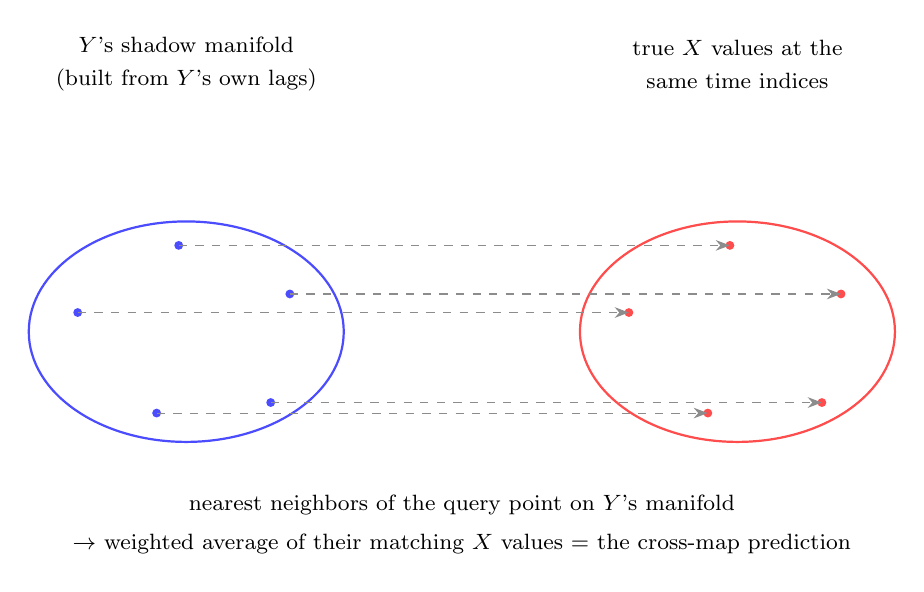
\begin{tikzpicture}
  \node[align=center] at (0,3.4) {\footnotesize $Y$'s shadow manifold\\\footnotesize (built from $Y$'s own lags)};
  \draw[thick, blue!70] (0,0) ellipse (2.0cm and 1.4cm);
  \foreach \i/\a in {1/20,2/95,3/170,4/250,5/320} {
    \coordinate (y\i) at ($(0,0)+({\a}:{1.1+0.3*mod(\i,2)})$);
    \fill[blue!70] (y\i) circle (1.6pt);
  }
  \node[align=center] at (7,3.4) {\footnotesize true $X$ values at the\\\footnotesize same time indices};
  \draw[thick, red!70] (7,0) ellipse (2.0cm and 1.4cm);
  \foreach \i/\a in {1/20,2/95,3/170,4/250,5/320} {
    \coordinate (x\i) at ($(7,0)+({\a}:{1.1+0.3*mod(\i,2)})$);
    \fill[red!70] (x\i) circle (1.6pt);
  }
  \foreach \i in {1,2,3,4,5} \draw[faintarrow] (y\i) -- (x\i);
  \node at (3.5,-2.2) {\footnotesize nearest neighbors of the query point on $Y$'s manifold};
  \node at (3.5,-2.7) {\footnotesize $\to$ weighted average of their matching $X$ values = the cross-map prediction};
\end{tikzpicture}
\caption{Cross-mapping schematic: does $Y$'s own shadow manifold let you recover $X$?}
\label{fig:ccm-schematic}
\end{figure}

\subsection{Algorithm: delay embedding, cross-map prediction, and the sweep}
\begin{steps}
\item \textbf{\_build\_delay\_embedding}: given a scalar series and $(E,\tau)$, build an $E$-column matrix where row $t$, column $d$ holds \texttt{series[t + d}$\cdot\tau$\texttt{]}; rows needing an out-of-bounds index are marked invalid, not zero-filled.
\item \textbf{\_crossmap\_predict}: draw $L$ library points (without replacement, $L$ = current sweep libSize); build a KD-tree over them; for every point in the full embedding, query $k{=}E{+}1$ nearest library neighbors, excluding any too close in \emph{time} (\texttt{exclusionRadius}); weight neighbors exponentially by distance, normalize, and predict as the weighted average of the target variable's values at those neighbors' time indices.
\item \textbf{proper\_ccm}: build both directions' embeddings once (columns$\to$target, c2t, and target$\to$columns, t2c); for each swept library size, repeat \texttt{ccm\_sample} independent random draws, scoring each direction with whichever metric \texttt{\_metric\_for} (Section~\ref{sec:target-metric}) resolves for that column; return the full \texttt{(sample}$\times$\texttt{libSize)} score matrix per direction.
\end{steps}

\subsection{Algorithm: the convergence gate}
\label{sec:convergence-gate}
\begin{steps}
\item Average per-sample scores at each library size; normalize the library-size axis to $[0,1]$; fit a line, take its slope.
\item \textbf{Pass} only if \emph{both}: the score at the largest library size exceeds the score at the smallest (sign-aware -- for \texttt{'mae'}, lower is better), \emph{and} the fitted slope exceeds \texttt{ccm\_slope} in the improving direction.
\item In \texttt{proper\_mde}'s own gate (Section~\ref{sec:mde-ccm-gate}), a failing candidate is simply rejected and the next-ranked one is tried. In the interaction matrix (\texttt{MODE='GMN'}), a failing pair's matrix cell is left at its pre-filled 0.
\end{steps}

\begin{figure}[h]
\centering
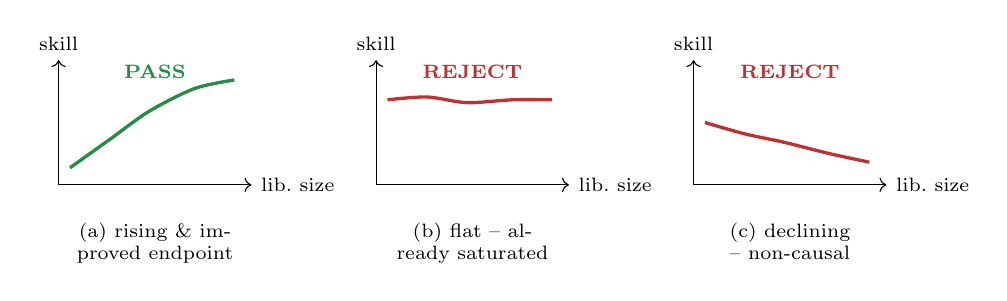
\begin{tikzpicture}[scale=0.72, every node/.style={font=\scriptsize}]
  \begin{scope}
    \draw[->] (0,0) -- (3.4,0) node[right]{lib.\ size};
    \draw[->] (0,0) -- (0,2.2) node[above]{skill};
    \draw[okline, very thick] plot[smooth] coordinates {(0.2,0.3) (0.9,0.8) (1.6,1.3) (2.4,1.7) (3.1,1.85)};
    \node[below, text width=3.0cm, align=center] at (1.7,-0.5) {(a) rising \& improved endpoint};
    \node[okline, font=\scriptsize\bfseries] at (1.7,2.0) {PASS};
  \end{scope}
  \begin{scope}[xshift=5.6cm]
    \draw[->] (0,0) -- (3.4,0) node[right]{lib.\ size};
    \draw[->] (0,0) -- (0,2.2) node[above]{skill};
    \draw[badline, very thick] plot[smooth] coordinates {(0.2,1.5) (0.9,1.55) (1.6,1.45) (2.4,1.5) (3.1,1.5)};
    \node[below, text width=3.0cm, align=center] at (1.7,-0.5) {(b) flat -- already saturated};
    \node[badline, font=\scriptsize\bfseries] at (1.7,2.0) {REJECT};
  \end{scope}
  \begin{scope}[xshift=11.2cm]
    \draw[->] (0,0) -- (3.4,0) node[right]{lib.\ size};
    \draw[->] (0,0) -- (0,2.2) node[above]{skill};
    \draw[badline, very thick] plot[smooth] coordinates {(0.2,1.1) (0.9,0.9) (1.6,0.75) (2.4,0.55) (3.1,0.4)};
    \node[below, text width=3.0cm, align=center] at (1.7,-0.5) {(c) declining -- non-causal};
    \node[badline, font=\scriptsize\bfseries] at (1.7,2.0) {REJECT};
  \end{scope}
\end{tikzpicture}
\caption{The convergence gate's three real shapes (Section~\ref{sec:history-noccm}): (a) is the textbook causal signature; (b) is what a too-large library window makes even genuinely causal pairs look like; (c) is what a non-causal or reverse-direction pair looks like.}
\label{fig:convergence-shapes}
\end{figure}

\subsection{Current calibration}
\label{sec:calibration}
\textbf{As of the window-sizing redesign (Section~\ref{sec:window-sizing}), \texttt{CCM\_WINDOW\_ROWS}/\texttt{CCM\_LIB\_SIZE\_PCTS} bound only \texttt{MODE='GMN'}'s own interaction matrix} -- \texttt{MODE='MDE-GMN'}'s own gate inside \texttt{proper\_mde} now sweeps \texttt{CCM\_LIB\_SIZES\_ROWS} (absolute row counts, Section~\ref{sec:window-sizing}) instead. \texttt{CCM\_WINDOW\_ROWS} (default \textbf{800}) bounds the row count \texttt{MODE='GMN'}'s own percentage-based library-size sweep is computed against; \texttt{CCM\_LIB\_SIZE\_PCTS} (default \textbf{2, 3, 5, 8, 20, 50} -- coarsened from an original 8-point grid, R17, after R9's own calibration sweep found the dropped points \texttt{12}/\texttt{30} already sat in the converged, uninformative tail at this window) gives absolute sizes of roughly 16--400 rows at that window -- the range where a real convergence curve was directly, empirically confirmed to exist (Section~\ref{sec:history-noccm}). \texttt{CCM\_SLOPE} (default \textbf{0.01}) is the minimum improving slope required, used by both modes; \texttt{CCM\_SAMPLE} (default \textbf{20}) is the resample count averaged per library size, likewise shared.
\pitfallbox{This gate is only as good as its calibration:}{Panel (b) above is not hypothetical -- it is what this pipeline's own interaction matrix looked like in production before recalibration. A flat curve is genuinely ambiguous (no real link, or a real link that already saturated before the smallest tested size); only testing library sizes small enough to see the rising part of a true curve can tell them apart. Treat any future change to \texttt{CCM\_WINDOW\_ROWS}/\texttt{CCM\_LIB\_SIZE\_PCTS} as a scientific calibration change, not a performance tweak.}

\newpage
% =====================================================================
\section{GMN Simulation via a Generalized S-map Embedding}
\label{sec:smap}
% =====================================================================

\subsection{Why gmn's own \texttt{Embed()} call had to be replaced}
\texttt{gmn.GMN} simulates every node with S-map, and its installed S-map branch calls \texttt{pyEDM.Embed(E, tau, columns)} -- one shared, uniform lag for every predictor. That is exactly what Stages 1--2 deliberately do \emph{not} produce: a node's real embedding is a list of (column, delay) pairs, potentially a different delay for every one. This pipeline monkeypatches \texttt{gmn.Node.\_\_init\_\_}, \texttt{gmn.Node.Forecast}, and \texttt{gmn.Node.Generate} to replace that call with \texttt{\_generalized\_embed()}, built directly from the graph.

\begin{figure}[H]
\centering
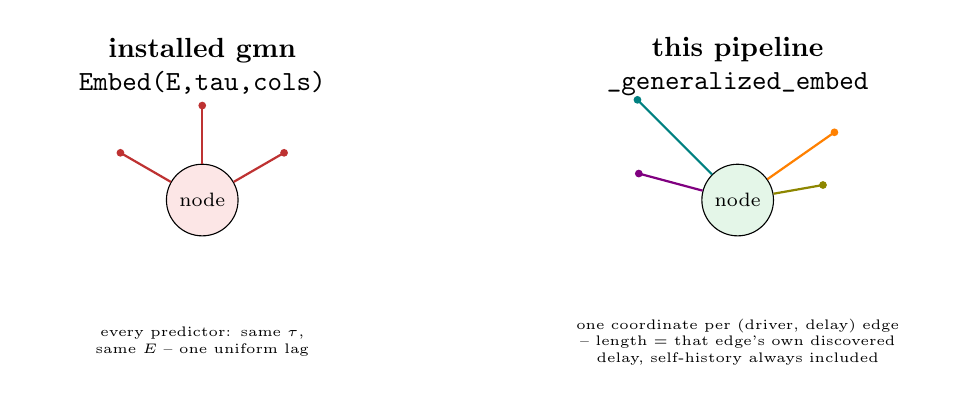
\begin{tikzpicture}[every node/.style={font=\scriptsize}]
  \node[font=\bfseries, align=center, text width=4.2cm] at (0.8,3.1) {installed gmn\\\texttt{Embed(E,tau,cols)}};
  \node[circle, draw, fill=badfill, minimum size=8mm] (nodeL) at (0.8,1.4) {node};
  \foreach \i/\a in {1/150,2/90,3/30}
    { \coordinate (pL\i) at ($(nodeL)+({\a}:1.2cm)$);
      \draw[badline, thick] (pL\i) -- (nodeL);
      \fill[badline] (pL\i) circle (1.4pt); }
  \node[font=\tiny, align=center, text width=3.6cm] at (0.8,-0.4) {every predictor: same $\tau$, same $E$ -- one uniform lag};

  \node[font=\bfseries, align=center, text width=4.6cm] at (7.6,3.1) {this pipeline\\\texttt{\_generalized\_embed}};
  \node[circle, draw, fill=okfill, minimum size=8mm] (nodeR) at (7.6,1.4) {node};
  \foreach \i/\a/\c/\len in {1/165/violet/0.8, 2/135/teal/1.3, 3/35/orange/1.0, 4/10/olive/0.6}
    { \coordinate (pR\i) at ($(nodeR)+({\a}:{\len cm+0.5cm})$);
      \draw[\c, thick] (pR\i) -- (nodeR);
      \fill[\c] (pR\i) circle (1.4pt); }
  \node[font=\tiny, align=center, text width=4.4cm] at (7.6,-0.4) {one coordinate per (driver, delay) edge -- length = that edge's own discovered delay, self-history always included};
\end{tikzpicture}
\caption{The embedding this patch replaces (left, one shared $(E,\tau)$ for every predictor) vs.\ what Stages 1--2 actually discovered (right, a genuinely non-uniform, per-driver-delay embedding) -- edge length here is schematic for delay magnitude, not to scale.}
\label{fig:embed-comparison}
\end{figure}

\subsection{Algorithm: \texttt{\_embedding\_spec\_for} and \texttt{\_generalized\_embed}}
\begin{steps}
\item \textbf{\texttt{MultiDiGraph} (\texttt{MODE='MDE-GMN'}):} a node's coordinates are its own delay=0 \textbf{anchor} (Section~\ref{sec:self-delay} -- unconditional on every node, but as of R14 \emph{only} the anchor, not the full old self-lag set) plus one coordinate per real in-edge, at that edge's own discovered delay -- see Section~\ref{sec:partition} for the fuller R14 story of why this changed and what it enables.
\item \textbf{Plain \texttt{DiGraph} (\texttt{MODE='GMN'}):} falls back to the original uniform scheme -- $E$ lagged copies of every predecessor plus itself, at the shared \texttt{fallback\_E}/\texttt{fallback\_tau} from that mode's own CCM grid search. R14 does not touch this branch at all -- \texttt{MODE='GMN'} never runs \texttt{build\_nested\_mde\_network()}, so it has no nested-MDE "discovered driver" concept to partition on in the first place.
\item \texttt{\_generalized\_embed} builds one column per (col, delay) pair, named \texttt{col(t-k)} (matching \texttt{pyEDM.Embed()}'s own naming convention), holding that column's value $|{\rm delay}|$ rows in the past; returns the frame with leading (now-\texttt{NaN}) rows dropped, plus \texttt{offset} -- the largest lag magnitude -- for callers realigning a time column.
\end{steps}

\begin{notebox}{The delay=0 anchor is unconditional; deeper self-lags are not.\label{sec:self-delay}}
Every node keeps its own delay=0 value as an unconditional anchor coordinate (Section~\ref{sec:partition} explains why this specific coordinate cannot be removed even though R14 removes the rest of the old self-history). \texttt{graph.graph['self\_delay\_set']} (set once in \texttt{build\_network()}, \texttt{sorted(set(lag\_set)} $\cup$ \texttt{\{0\}, reverse=True)}) still exists post-R14, but only as an upper bound on any node's real embedding offset (\texttt{network\_max\_embedding\_offset()}, used to size a network-wide \texttt{Forecast()} lib/pred window) -- it is no longer unioned into any node's actual embedding content the way it was before R14.
\end{notebox}

\begin{notebox}{Replaces this pipeline's own earlier, narrower patch (\texttt{\_fixed\_node\_forecast}):}
Before the redesign, this pipeline patched only \texttt{gmn.Node.Forecast} for two confirmed \texttt{gmn} bugs: (1) \texttt{gmn/Forecast.py} calls \texttt{Embed()} without ever importing \texttt{pyEDM.Embed} in that module, raising \texttt{NameError} on the first S-map \texttt{Forecast()} call; (2) the divergence check \texttt{val.max() > 1E15} treats \texttt{val} -- a 2-tuple \texttt{(time, predictions)} -- as if it had a \texttt{.max()} method, raising \texttt{AttributeError} unconditionally. The generalized-embedding patch above fixes both as a side effect (it no longer calls \texttt{pyEDM.Embed()} at all, and checks the predictions Series directly) while also covering \texttt{Generate()} and \texttt{\_\_init\_\_}, which the narrower patch never touched. Every other \texttt{FunctionType} branch (Simplex, kedmSimplex, Linear, SVR, knn) is copied verbatim from the installed package, unused here since every node is S-map, but kept intact so the patch cannot silently change behavior for a future non-S-map code path.
\end{notebox}

\linknote{\texttt{gmn.GMN} can now simulate this pipeline's genuinely non-uniform network at \emph{any} choice of per-node theta. Nothing so far has decided which theta is best -- that's the search, Section~\ref{sec:search}.}

\newpage
% =====================================================================
\section{Hyperparameter Search: Theta and the Generate() Start Row}
\label{sec:search}
% =====================================================================

\subsection{Why this search replaced a full $(E,\tau,\theta)$ grid}
Before the redesign, this pipeline searched \texttt{SMAP\_SEARCH\_MODE='coarse\_retune'}/\texttt{'joint'} -- a full grid over \texttt{E\_RANGE}$\times$\texttt{TAU\_RANGE}, retuning theta at every $(E,\tau)$ candidate, because $E$ and $\tau$ were otherwise unknowns (Section~\ref{sec:history-port}). Now $E$ and every driver's delay come directly from Stages 1--2's own discovered graph (Section~\ref{sec:smap}) -- there is nothing left to grid-search except $\theta$, S-map's own localization parameter. This is a genuine reduction in search cost: the old search's dominant cost (\texttt{len(E)}$\times$\texttt{len(tau)} full \texttt{Generate()} calls) becomes one \texttt{Generate()} call per network.

\begin{figure}[H]
\centering
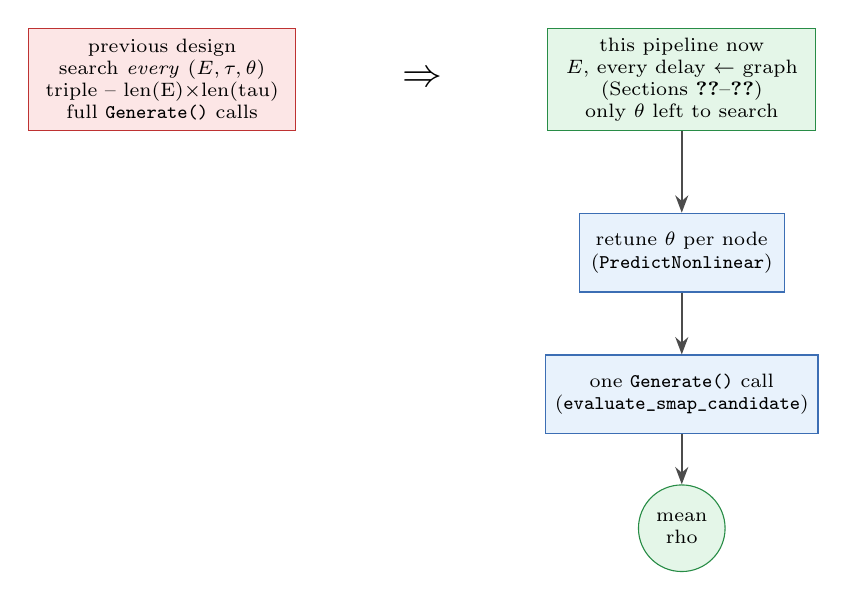
\begin{tikzpicture}[every node/.style={font=\scriptsize}]
  \node[rectangle, draw=badline, fill=badfill, minimum width=3.4cm, minimum height=1.3cm, align=center] (old) at (0,0) {previous design\\search \emph{every} $(E,\tau,\theta)$\\triple -- len(E)$\times$len(tau)\\full \texttt{Generate()} calls};
  \node[rectangle, draw=okline, fill=okfill, minimum width=3.4cm, minimum height=1.3cm, align=center] (new) at (6.6,0) {this pipeline now\\$E$, every delay $\leftarrow$ graph\\(Sections~\ref{sec:stage1}--\ref{sec:stage2})\\only $\theta$ left to search};
  \node[font=\Large] at (3.3,0) {$\Rightarrow$};
  \node[rectangle, draw=stageline, fill=stagefill, minimum width=2.6cm, minimum height=1cm, align=center] (retune) at (6.6,-2.2) {retune $\theta$ per node\\(\texttt{PredictNonlinear})};
  \node[rectangle, draw=stageline, fill=stagefill, minimum width=2.6cm, minimum height=1cm, align=center] (gen) at (6.6,-4.0) {one \texttt{Generate()} call\\(\texttt{evaluate\_smap\_candidate})};
  \node[circle, draw=okline, fill=okfill, minimum size=1.1cm, align=center] (score) at (6.6,-5.7) {mean\\rho};
  \draw[arrow] (new) -- (retune);
  \draw[arrow] (retune) -- (gen);
  \draw[arrow] (gen) -- (score);
\end{tikzpicture}
\caption{What the search used to cost (left) vs.\ what it costs now (right): a full grid collapses to one retune-then-score loop per network.}
\label{fig:search-reduction}
\end{figure}

\subsection{Algorithm: \texttt{retune\_theta\_for\_all\_nodes}}
For every \emph{simulated} node (Section~\ref{sec:partition}'s \texttt{\_simulated\_nodes(graph)} -- a \texttt{'real\_data'}-mode external input has no embedding to retune and is correctly excluded), build its generalized embedding directly (not through a live \texttt{gmn.Node} -- this runs before any \texttt{gmn.GMN} object exists), split 70/30, and sweep \texttt{THETA\_RANGE} to find the score-maximizing $\theta$ (R20's \texttt{proper\_predict\_nonlinear}, below, in place of \texttt{pyEDM.PredictNonlinear}). Falls back to $\theta=3$ whenever there's too little data for a meaningful split (fewer than \texttt{min\_pred\_rows=20} prediction rows) or the sweep itself fails.

\decisionbox{R20: a TSLS-aware theta search, closing a gap this document previously reported as unaddressed:}{\texttt{PredictNonlinear} scored purely by \texttt{pyEDM}'s own internal Pearson-rho, regardless of \texttt{METRIC} -- the one scoring call site in the whole pipeline that didn't route through \texttt{\_metric\_for()} (Section~\ref{sec:target-metric}). Reading \texttt{PredictNonlinear}'s own source first (rather than writing a new S-map engine outright) found it is already nothing more than a thin sweep: per candidate $\theta$, one \texttt{pyEDM.SMap(...)} call, scored via \texttt{ComputeError(...)['rho']}, with the predictions themselves discarded -- there is no separate "S-map engine" hidden inside it to reimplement, and \texttt{ComputeError}'s own \texttt{rho} is confirmably the identical Pearson-correlation formula \texttt{\_score(kind='correlation')} already uses. \texttt{proper\_predict\_nonlinear()} (new, this pipeline file, not \texttt{cleaned\_helper\_functions.py} -- which stays deliberately \texttt{pyEDM}-free) is therefore a thin wrapper: call \texttt{pyEDM.SMap(...)} directly (the same compiled S-map \texttt{gmn}'s own \texttt{Generate()}/\texttt{Forecast()} already calls at runtime, so this doesn't add a second S-map implementation to trust), and score its returned predictions via \texttt{tsls.\_score(metric, ...)} instead of \texttt{ComputeError}. \texttt{retune\_theta\_for\_all\_nodes()} now resolves each node's own metric via \texttt{\_metric\_for()} -- \texttt{'f1'} for a neuron node, \texttt{'correlation'} for a target -- before calling it. \textbf{Validated by direct equivalence}, not merely by analogy: on a real chaotic delay embedding, \texttt{proper\_predict\_nonlinear(metric='correlation')} selects the identical best theta as \texttt{pyEDM.PredictNonlinear}, with every theta's own score matching \texttt{PredictNonlinear}'s own rho to $<10^{-6}$ across the whole grid, not just at the maximum.}

\subsection{Algorithm: \texttt{run\_theta\_search} and \texttt{evaluate\_smap\_candidate}}
Retunes theta (above), then scores the result with exactly one \texttt{Generate()} call via \texttt{evaluate\_smap\_candidate()} -- mean score across \emph{targets only} (not driver nodes), via \texttt{tsls.\_score(metric=target\_metric)} (Section~\ref{sec:target-metric}), between the simulated and real held-out series, starting at \texttt{GENERATE\_VALIDATION\_START} (never \texttt{PREDICTION\_START} -- the leakage guard applies here too). Guarded with try/except: \texttt{gmn.Generate()} can raise \texttt{RuntimeError} on SMap divergence ($>10^{15}$) even at a retuned theta on a large network -- a real, expected outcome for some configurations, not a bug to crash the whole search over.

\subsection{Algorithm: \texttt{sweep\_generate\_start}}
\texttt{Generate()} is a recursive nonlinear simulation, so which row it launches from can change how well it tracks reality, independent of how good the embedding/theta are. This sweep tries \texttt{GENERATE\_START\_MIN/MAX/STEP\_OFFSET} candidate offsets from \texttt{GENERATE\_VALIDATION\_START} (always $\ge 0$), scores each with the same \texttt{evaluate\_smap\_candidate()} objective, and keeps the best. A single-offset default (\texttt{MIN=0, MAX=1}) disables the sweep entirely -- \texttt{rebuild\_at\_best\_params()} is about to run \texttt{Generate()} at that exact configuration anyway.

\begin{figure}[H]
\centering
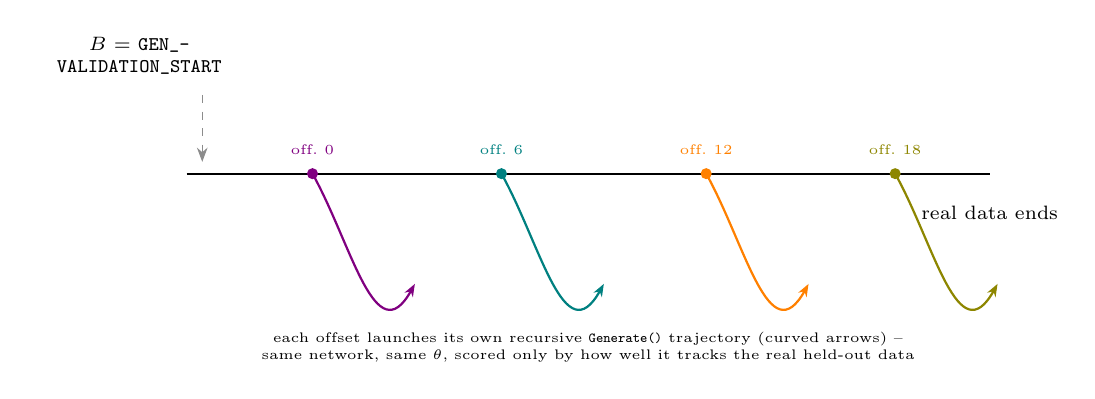
\begin{tikzpicture}[every node/.style={font=\scriptsize}]
  \draw[thick] (0,0) -- (10.2,0);
  \node[align=center, text width=2.6cm] at (-0.6,1.5) {$B$ = \texttt{GEN\_VALIDATION\_START}};
  \draw[faintarrow] (0.2,1.0) -- (0.2,0.15);
  \node[align=center] at (10.2,-0.5) {real data ends};
  \foreach \x/\c/\lab in {1.6/violet/{off.\ 0}, 4.0/teal/{off.\ 6}, 6.6/orange/{off.\ 12}, 9.0/olive/{off.\ 18}} {
    \fill[\c] (\x,0) circle (2pt);
    \draw[\c, thick, -{Stealth[length=1.6mm]}] (\x,0) .. controls +(0.5,-0.9) and +(-0.5,-0.9) .. (\x+1.3,-1.4);
    \node[font=\tiny, \c] at (\x,0.3) {\lab};
  }
  \node[font=\tiny, align=center, text width=8.6cm] at (5.1,-2.2) {each offset launches its own recursive \texttt{Generate()} trajectory (curved arrows) -- same network, same $\theta$, scored only by how well it tracks the real held-out data};
\end{tikzpicture}
\caption{The start-point sweep, schematically: the identical model, launched from several different rows within $[B,\mathrm{end})$, can track reality very differently.}
\label{fig:start-sweep-schematic}
\end{figure}

\pitfallbox{Checkpointing here is intra-job only, unlike the cross-job cache (Section~\ref{sec:storage}):}{\texttt{sweep\_generate\_start()} writes a pickle checkpoint to \texttt{results\_dir} after every offset so a job that dies mid-sweep can resume \emph{within the same submission}. The cross-job fingerprinted cache (\texttt{reuse\_cache}/\texttt{RUN\_CACHE\_DIR}) is a separate, additional mechanism that lets a full resubmission after a crash skip the whole sweep -- see Section~\ref{sec:storage}.}

\newpage
% =====================================================================
\section{Final Validation}
\label{sec:validation}
% =====================================================================
Three independent diagnostics, deliberately not collapsed into one number, so a network that looks good on one metric but not another is visible rather than averaged away.

\begin{figure}[H]
\centering
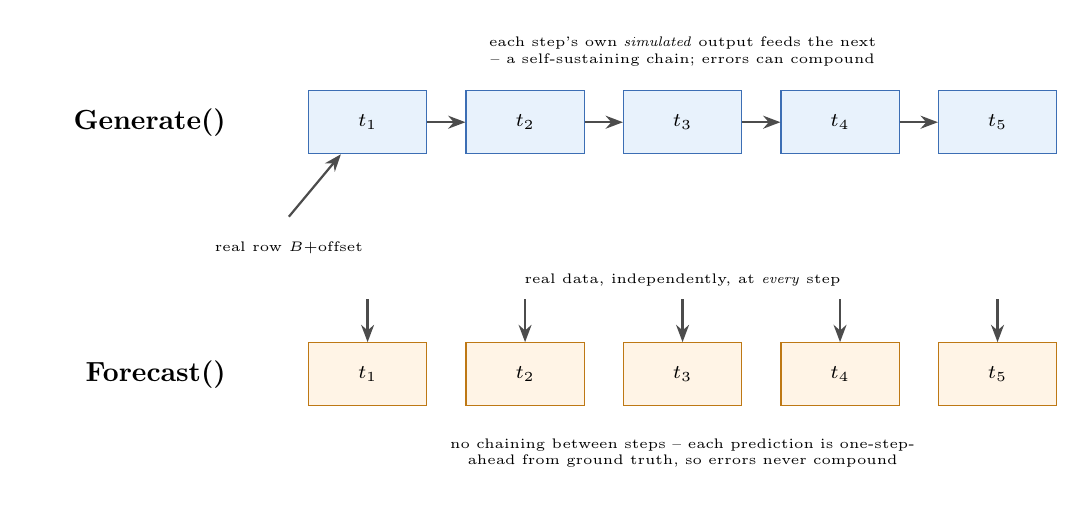
\begin{tikzpicture}[every node/.style={font=\scriptsize}]
  \node[align=right, font=\bfseries, text width=2.4cm] at (-3.0,2.2) {Generate()};
  \foreach \i/\x in {1/0,2/2,3/4,4/6,5/8}
    \node[rectangle, draw=stageline, fill=stagefill, minimum width=1.5cm, minimum height=0.8cm] (g\i) at (\x,2.2) {$t_{\i}$};
  \draw[arrow] (-1.0,1.0) -- (g1);
  \node[font=\tiny] at (-1.0,0.6) {real row $B{+}$offset};
  \foreach \i/\j in {1/2,2/3,3/4,4/5} \draw[arrow] (g\i) -- (g\j);
  \node[font=\tiny, text width=8.6cm, align=center] at (4,3.1) {each step's own \emph{simulated} output feeds the next -- a self-sustaining chain; errors can compound};

  \node[align=right, font=\bfseries, text width=2.4cm] at (-3.0,-1.0) {Forecast()};
  \foreach \i/\x in {1/0,2/2,3/4,4/6,5/8}
    \node[rectangle, draw=stage2line, fill=stage2fill, minimum width=1.5cm, minimum height=0.8cm] (f\i) at (\x,-1.0) {$t_{\i}$};
  \foreach \i/\x in {1/0,2/2,3/4,4/6,5/8}
    \draw[arrow] (\x,-0.05) -- (f\i);
  \node[font=\tiny] at (4,0.2) {real data, independently, at \emph{every} step};
  \node[font=\tiny, text width=8.6cm, align=center] at (4,-2.0) {no chaining between steps -- each prediction is one-step-ahead from ground truth, so errors never compound};
\end{tikzpicture}
\caption{Why both diagnostics matter: \texttt{Generate()} tests whether the network can sustain itself free-running; \texttt{Forecast()} tests one-step skill in isolation, with real data reinjected at every step. A network can score well on one and poorly on the other. Section~\ref{sec:outputs} shows a real \texttt{Forecast()} guard rejection.}
\label{fig:generate-vs-forecast}
\end{figure}

\subsection{Algorithm: \texttt{rebuild\_at\_best\_params}}
Reruns \texttt{Generate()} once more at the search's winning theta and start row. Guarded per-network: a divergence here is logged and that network is skipped rather than crashing the whole job. R11 additionally writes \texttt{per\_node\_scores\_\{network\_id\}.csv} (node, role -- \texttt{TARGET}/\texttt{driver}, metric, score) alongside the existing per-node print -- purely additive, computed \emph{after} theta/start-row are already final, so it changes nothing about what the search itself optimized for.
\decisionbox{R11 confirmed the search objective stays target-only, per-node reporting notwithstanding:}{\texttt{evaluate\_smap\_candidate()}'s own score (what \texttt{run\_theta\_search()}/\texttt{sweep\_generate\_start()} both actually optimize) averages only \texttt{net\_result['targets']}' own scores -- never a driver node's, never mixed with \texttt{METRIC}. The per-node CSV above is a reporting addition on top of that unchanged objective, not a second objective.}

\subsection{Algorithm: \texttt{run\_forecast\_diagnostic}}
Runs \texttt{Forecast()} at the same winning parameters and plots it alongside the free-running \texttt{Generate()} trace and the real data (\texttt{FORECAST\_PLOT\_RANGE='full'} or \texttt{'windowed'}). Separates two failure modes: a network that forecasts well one step ahead but diverges when run freely has an \emph{accumulation} problem, not a one-step prediction problem.

\subsection{Algorithm: \texttt{gmn\_fidelity\_rho}}
For every node: build a two-column (simulated, real) table at matching time indices, run a Simplex prediction of "real" from "simulated" scored via \texttt{tsls.\_score()} with each node's own correctly-resolved metric (Section~\ref{sec:target-metric}), and score it. This is a Fig-4e-style generative fidelity check: it asks not "did the curves look similar" but "does the simulated trajectory's own internal dynamics let you recover the real one."

\begin{figure}[H]
\centering
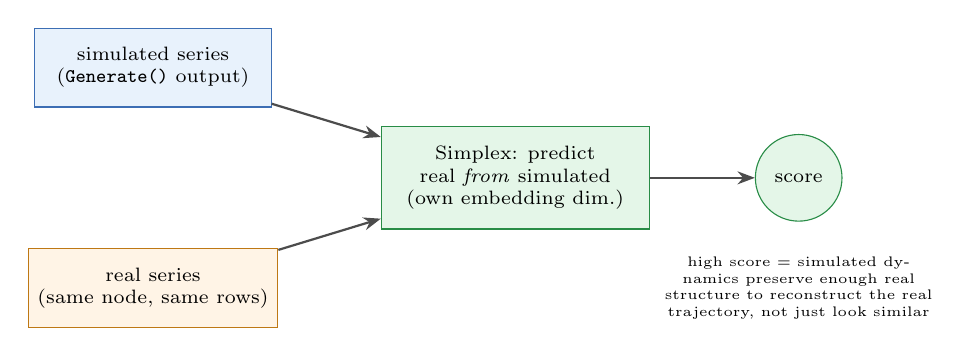
\begin{tikzpicture}[every node/.style={font=\scriptsize}]
  \node[rectangle, draw=stageline, fill=stagefill, minimum width=3cm, minimum height=1cm, align=center] (sim) at (0,1.4) {simulated series\\(\texttt{Generate()} output)};
  \node[rectangle, draw=stage2line, fill=stage2fill, minimum width=3cm, minimum height=1cm, align=center] (real) at (0,-1.4) {real series\\(same node, same rows)};
  \node[rectangle, draw=okline, fill=okfill, minimum width=3.4cm, minimum height=1.3cm, align=center] (simplex) at (4.6,0) {Simplex: predict\\real \emph{from} simulated\\(own embedding dim.)};
  \draw[arrow] (sim) -- (simplex);
  \draw[arrow] (real) -- (simplex);
  \node[circle, draw=okline, fill=okfill, minimum size=1.1cm] (rho) at (8.2,0) {score};
  \draw[arrow] (simplex) -- (rho);
  \node[font=\tiny, text width=3.6cm, align=center] at (8.2,-1.4) {high score = simulated dynamics preserve enough real structure to reconstruct the real trajectory, not just look similar};
\end{tikzpicture}
\caption{The Fig-4e-style fidelity metric: a structure-aware test, stricter than a plain correlation between the two curves.}
\label{fig:fidelity-schematic}
\end{figure}

\linknote{These three diagnostics are the pipeline's actual deliverable for \texttt{MODE='MDE-GMN'}. Section~\ref{sec:diagnostics} is optional, MDE-specific tooling that inspects the \emph{selection process} itself, not part of the causal claim.}

\newpage
% =====================================================================
\section{Stage 6: MDE-only Diagnostics}
\label{sec:diagnostics}
% =====================================================================
(Skipped when \texttt{MODE='GMN'}. \texttt{run\_tp\_vs\_rho\_sweep}/\texttt{run\_univariate\_e\_tau\_grid}/\texttt{plot\_3d\_mde\_projection} below are controlled by \texttt{RUN\_MDE\_DIAGNOSTICS}; \texttt{run\_mde\_evaluate} (Section~\ref{sec:mde-evaluate}) is controlled by its own, deliberately separate \texttt{RUN\_MDE\_EVALUATE} toggle.)

\subsection{\texttt{run\_tp\_vs\_rho\_sweep} and \texttt{run\_univariate\_e\_tau\_grid}}
For each target, using its MDE-selected columns as a fixed embedding, sweep the prediction horizon $T_p$ from 1 to \texttt{MAX\_TP} via \texttt{proper\_predict\_interval} (predictability-horizon diagnostic; skipped per-target with a print, not a crash, if that target selected zero columns), and a univariate self-prediction $(E,\tau)$ grid per target via \texttt{estimate\_node\_dimension}'s own machinery, heatmapped with any cell above \texttt{GRID\_RHO\_THRESHOLD} boxed.
\pitfallbox{Two real gaps found and fixed here (R7), one still open:}{Review confirmed \texttt{run\_tp\_vs\_rho\_sweep}'s shared figure used to call \texttt{savefig()} unconditionally even when every target had zero selected columns, writing an empty PNG with an empty legend -- fixed with a per-target zero-columns skip plus a guard around \texttt{savefig()} itself. Separately, \texttt{run\_univariate\_e\_tau\_grid} unconditionally dereferenced \texttt{r['mde\_df']}, and a target whose depth-0 MDE call itself \emph{raised} (rather than legitimately selecting zero drivers) gets \texttt{mde\_df=None} -- this crashed the \emph{whole function}, taking every other target's own perfectly computable figure down with it, right before the final \texttt{"Pipeline complete"} print. Fixed with a per-target \texttt{if mde\_df is None: continue} guard (deliberately \emph{not} gated on zero selected columns -- this function's univariate grid is meaningful even for a legitimate zero-driver target; only the actual crash-causing condition is guarded). \textbf{Still open, found later and not yet closed}: neither function wraps its own actual computation (\texttt{proper\_predict\_interval}/\texttt{proper\_simplex}) in an exception guard -- only the precondition that produced the two bugs above is checked. A target that passes both preconditions but whose call raises for some other reason would still crash the whole function today (Section~\ref{sec:limitations}).}

\begin{figure}[H]
\centering
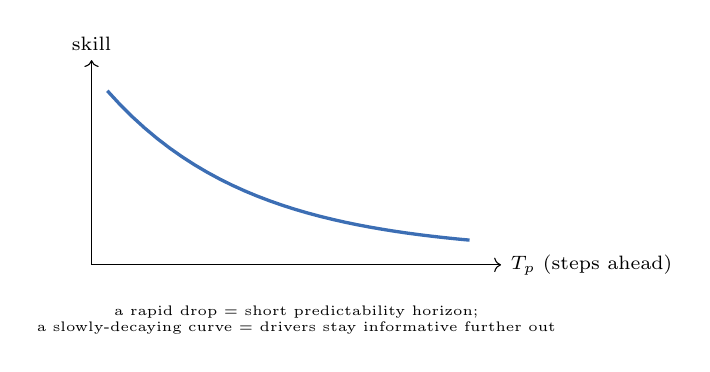
\begin{tikzpicture}[every node/.style={font=\scriptsize}]
  \draw[->] (0,0) -- (5.2,0) node[right] {$T_p$ (steps ahead)};
  \draw[->] (0,0) -- (0,2.6) node[above] {skill};
  \draw[stageline, very thick, domain=0.2:4.8, samples=30] plot ({\x}, {2.3*exp(-0.55*\x)+0.15});
  \node[font=\tiny, align=center] at (2.6,-0.7) {a rapid drop = short predictability horizon;\\a slowly-decaying curve = drivers stay informative further out};
\end{tikzpicture}
\caption{\texttt{run\_tp\_vs\_rho\_sweep}, schematically: how far into the future a target's MDE-selected drivers remain informative, independent of the network's own \texttt{Generate()} fidelity.}
\label{fig:tp-sweep-schematic}
\end{figure}

\subsection{\texttt{plot\_3d\_mde\_projection}}
For the first two targets jointly: a 3D scatter of (first target, its own top-2 MDE-selected real observables), colored by the second target's value at each row -- a purely visual sanity check of whether the target and its selected drivers trace out any visible joint structure. Figure~\ref{fig:3d-projection} (Section~\ref{sec:outputs}) is real output from this exact function.

\subsection{\texttt{run\_mde\_evaluate}: MDE vs.\ unsupervised baselines (R19)}
\label{sec:mde-evaluate}
The sibling pipeline's own \texttt{run\_mde\_evaluate} compares \texttt{dimx.Evaluate}'s reconstruction-quality metrics for MDE's own selection against two unsupervised baselines (PCA and diffusion-map embeddings) of the same candidate pool -- this pipeline had no equivalent for a long time (\texttt{dimx.Evaluate} depends on the \texttt{dimx.MDE} result object \texttt{proper\_mde} never builds). R19 closed this gap with a from-scratch reimplementation against \texttt{proper\_simplex}/\texttt{sklearn.decomposition.PCA}/\texttt{sklearn.linear\_model.LinearRegression}/\texttt{pydiffmap.diffusion\_map} directly -- not a port, and not a call into \texttt{dimx} at all, since this pipeline has no \texttt{dimx} import to route through. \texttt{dimx.Evaluate.CAE()} was read directly from its own source to recover the exact metric definition (\texttt{sum(abs(x - y))} -- an unnormalized cumulative absolute error, not a mean or a fraction) rather than reimplementing from the name alone, and reproduced verbatim as \texttt{\_cae()}.
\begin{steps}
\item \textbf{$D$ and the driver pool.} $D$ is the number of direct drivers of the target -- read from the completed network graph (\texttt{net\_result['network']['Graph']}), never a depth-0-only selection list. For a $>1$-target group (\texttt{GMN\_MODE='combined'}), $D$ is the \emph{union} of every target's own direct-driver set. PCA/diffusion-map both fit on the network-wide driver pool (\texttt{DATA\_AFTER\_MDE} -- every observable nested-MDE kept \emph{anywhere} in the whole network, a superset of any one target's own direct drivers whenever Stage 2 chains through an intermediate node), the same ground-truth file every other diagnostic in this file already reads.
\item \textbf{Fit and predict.} MDE: \texttt{proper\_simplex} on each target's own direct-driver embedding. PCA/diffusion-map: extract the first $D$ components of the driver pool, then \texttt{LinearRegression} onto the target(s) -- in combined mode, \texttt{sklearn}'s own native multi-output regression fits \emph{one} shared component basis and regresses it onto \emph{both} targets at once (confirmed against \texttt{sklearn}'s own documented behavior, not assumed), producing a 2-column prediction directly; MDE has no multivariate equivalent, so its own two single-target reconstructions are combined into one $(x,y)$ trajectory for the figure's spatial panel.
\item \textbf{Score and plot.} Every method is scored by CAE and by \texttt{tsls.\_score(..., target\_metric, ...)} (Section~\ref{sec:target-metric}) over the held-out MDE validation segment $[A, A{+}(B{-}A))$ -- the same segment \texttt{evaluate\_smap\_candidate()} and every other MDE-side diagnostic already use, never the Generate/Forecast segment $[B,\mathrm{end})$. The figure is 4 stacked time-series panels (Predictions/MDE-drivers/D-Map-projection/PCA-projection) for a 1-target group, or a spatial $(x,y)$ trajectory as panel 1 (confirmed by explicit user decision, since the reference figure this was built against was single-target and didn't settle the question) for a 2-target group.
\end{steps}

\begin{figure}[h]
\centering
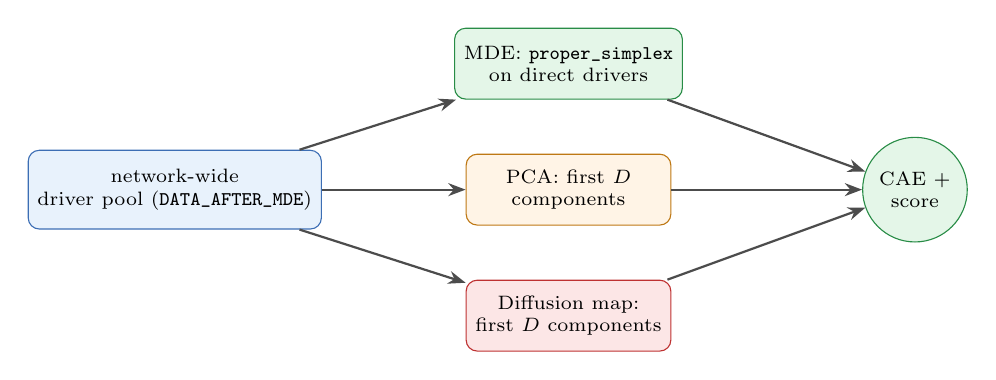
\begin{tikzpicture}[every node/.style={font=\scriptsize}]
  \node[rectangle, draw=stageline, fill=stagefill, rounded corners, minimum width=3.2cm, minimum height=1cm, align=center] (pool) at (0,0) {network-wide\\driver pool (\texttt{DATA\_AFTER\_MDE})};
  \node[rectangle, draw=okline, fill=okfill, rounded corners, minimum width=2.6cm, minimum height=0.9cm, align=center] (mde) at (5.0,1.6) {MDE: \texttt{proper\_simplex}\\on direct drivers};
  \node[rectangle, draw=stage2line, fill=stage2fill, rounded corners, minimum width=2.6cm, minimum height=0.9cm, align=center] (pca) at (5.0,0) {PCA: first $D$\\components};
  \node[rectangle, draw=badline, fill=badfill, rounded corners, minimum width=2.6cm, minimum height=0.9cm, align=center] (dmap) at (5.0,-1.6) {Diffusion map:\\first $D$ components};
  \draw[arrow] (pool) -- (mde);
  \draw[arrow] (pool) -- (pca);
  \draw[arrow] (pool) -- (dmap);
  \node[circle, draw=okline, fill=okfill, minimum size=1.0cm, align=center] (score) at (9.4,0) {CAE +\\score};
  \draw[arrow] (mde) -- (score);
  \draw[arrow] (pca) -- (score);
  \draw[arrow] (dmap) -- (score);
\end{tikzpicture}
\caption{\texttt{run\_mde\_evaluate}: the same driver pool, reconstructed three independent ways, scored on equal footing -- MDE's causally-gated selection against two unsupervised baselines that never see the causality gate at all.}
\label{fig:mde-evaluate}
\end{figure}

\subsection{The \texttt{RUN\_MDE\_EVALUATE} toggle: why this diagnostic defaults off}
\label{sec:mde-evaluate-toggle}
Running the smoke configuration on real cluster data (job 40143104, after the metric-routing/window-sizing/CCM-gate fixes and the progress-monitoring log, Section~\ref{sec:progress-log}, all landed) completed Stage 1, Stage 2, theta retuning, the \texttt{Generate()} rebuild, \texttt{Forecast()}, and \S\ref{sec:diagnostics}'s first two diagnostics cleanly -- then crashed inside \texttt{run\_mde\_evaluate()}'s diffusion-map baseline.
\begin{steps}
\item \textbf{The crash, root cause isolated.} \texttt{ValueError: Input X contains infinity...} inside the diffusion-map regression step. Reproduced in isolation on the real crashed job's own saved data: crashes identically at 800 rows \emph{and} at the full $\sim$31{,}000-row scale in 1.8s -- directly refuting a point-count/window-size explanation before it could be accepted as one. Instrumented \texttt{pydiffmap}'s own kernel row-sums directly: on held-out (prediction) points, 53\% had a kernel row-sum of exactly zero, because those points' own TSLS values exceeded the \emph{library}'s observed range entirely -- no k-nearest-neighbor kernel similarity above float underflow exists for them, at any epsilon (confirmed \texttt{pydiffmap}'s own generous automatic-epsilon selection does not avoid this). A real, non-rare property of this data: \textbf{9/45 (20\%) of real channels} show this "held-out exceeds library range" pattern -- channel-level firing-rate non-stationarity across the recording, not a one-off unlucky column.
\item \textbf{The hang, mechanism explicitly not diagnosed.} Verifying an exception guard alone (below) against the same real data at its own $\sim$31{,}000-row scale did not crash -- it ran for \textbf{74+ minutes of CPU time with no completion, no crash, and no output}, before being killed manually. A \texttt{try/except} only protects against something that actually raises; this never did. TSLS's own duplicate-row structure (long inter-spike ramps are locally near-identical, by construction) is suspected but unconfirmed as a contributing factor -- and because it is intrinsic to TSLS itself, not to this dataset or \texttt{REGION\_CHANNEL\_CAP}, it could plausibly affect other KD-tree- or kernel-based computations on TSLS series elsewhere in this codebase. Whether the fast crash and the slow hang are one underlying pathology surfacing differently, or two distinct issues, is itself unresolved -- diagnosing this is its own, separate future task (Section~\ref{sec:future}).
\end{steps}

\begin{figure}[h]
\centering
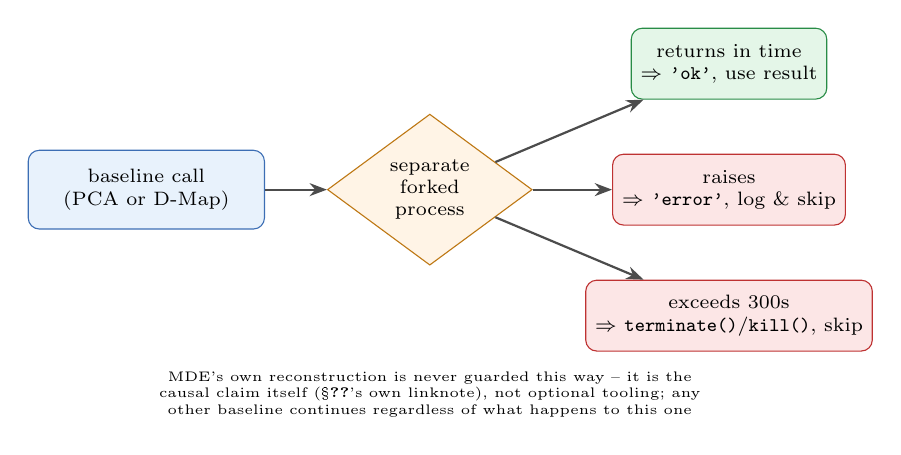
\begin{tikzpicture}[every node/.style={font=\scriptsize}]
  \node[rectangle, draw=stageline, fill=stagefill, rounded corners, minimum width=3.0cm, minimum height=1cm, align=center] (call) at (0,0) {baseline call\\(PCA or D-Map)};
  \node[diamond, draw=stage2line, fill=stage2fill, minimum width=2.6cm, minimum height=1.8cm, align=center, inner sep=1pt] (fork) at (3.6,0) {separate\\forked\\process};
  \node[rectangle, draw=okline, fill=okfill, rounded corners, minimum width=2.4cm, minimum height=0.9cm, align=center] (ok) at (7.4,1.6) {returns in time\\$\Rightarrow$ \texttt{'ok'}, use result};
  \node[rectangle, draw=badline, fill=badfill, rounded corners, minimum width=2.4cm, minimum height=0.9cm, align=center] (crash) at (7.4,0) {raises\\$\Rightarrow$ \texttt{'error'}, log \& skip};
  \node[rectangle, draw=badline, fill=badfill, rounded corners, minimum width=2.6cm, minimum height=0.9cm, align=center] (timeout) at (7.4,-1.6) {exceeds 300s\\$\Rightarrow$ \texttt{terminate()}/\texttt{kill()}, skip};
  \draw[arrow] (call) -- (fork);
  \draw[arrow] (fork) -- (ok);
  \draw[arrow] (fork) -- (crash);
  \draw[arrow] (fork) -- (timeout);
  \node[font=\tiny, align=center, text width=9.5cm] at (3.6,-2.6) {MDE's own reconstruction is never guarded this way -- it is the causal claim itself (\S\ref{sec:validation}'s own linknote), not optional tooling; any other baseline continues regardless of what happens to this one};
\end{tikzpicture}
\caption{The fix: each baseline runs in its own forked process, independently exception-guarded and wall-clock bounded -- protecting against both the fast crash and the non-raising hang, without requiring the hang's own mechanism to be understood first.}
\label{fig:mde-evaluate-guard}
\end{figure}

\decisionbox{The fix: a dedicated toggle, an independent guard per baseline, and a subprocess-based wall-clock bound:}{\texttt{RUN\_MDE\_EVALUATE} (default \textbf{false}), deliberately separate from \texttt{RUN\_MDE\_DIAGNOSTICS} -- \S\ref{sec:diagnostics}'s other two diagnostics are unaffected by either failure mode and keep running under the existing knob regardless. When off, this is logged exactly once per run, unconditionally, in both the console output and the progress log (Section~\ref{sec:progress-log}) -- a silent absence is exactly how the swallowed-exception history (Section~\ref{sec:history-metric-bug}) went unnoticed for as long as it did. PCA and diffusion-map each get their own independent exception guard: a failure is logged with the exception text and the target(s) it occurred on, and only that baseline's own numbers/plot panel are skipped. Underneath the guard, each baseline now runs in a genuinely separate \texttt{multiprocessing.Process} (fork), force-killed (\texttt{terminate()}, then \texttt{kill()}) if it exceeds \texttt{MDE\_EVALUATE\_BASELINE\_TIMEOUT\_SECONDS} (default \textbf{300}) -- a plain \texttt{try/except} plus a signal-based "soft" timeout would not have been enough, since the hang can occur inside compiled KD-tree/BLAS calls that don't return control to the Python interpreter for a long stretch, exactly when a signal fires but its handler cannot run until the call returns on its own. Only an OS-level kill of a separate process reclaims control regardless of what the computation is doing internally -- cost: one process fork per baseline call (cheap under \texttt{fork}) plus a hard kill on timeout discards whatever progress a slow-but-would-eventually-succeed computation had made, a deliberate trade for a bounded worst case over an unbounded one. 300s is not calibrated against a known-good completion time (none has yet been observed at real scale) -- chosen as generous headroom over the 1.8s a genuine crash takes to surface.}

\pitfallbox{\texttt{RUN\_MDE\_EVALUATE=false} widens a gap, it does not close one:}{This diagnostic exists and works (verified bit-identical against its pre-guard baseline on the reference/toy data it was validated against) but is off by default pending the hang's own diagnosis -- Section~\ref{sec:capabilities}'s "cannot compare MDE's selection against an unsupervised baseline" gap is therefore \emph{wider} than it was before R19, not narrower, until this is re-enabled. Exposed (for naming consistency only) in the sibling pipeline's own sbatch script too, but not wired into \texttt{simple-mde-gmn.py}'s own \texttt{dimx.Evaluate}-based \texttt{run\_mde\_evaluate} -- that implementation operates on raw spike counts, not TSLS, and has not been confirmed to share this finding's own suspected mechanism.}

\newpage
% =====================================================================
\section{The TSLS-Aware Scoring Framework}
\label{sec:scoring}
% =====================================================================
Every algorithm above that needs to say "how good was this prediction" routes through one shared framework, so a single design decision (which metric to use, and for which kind of column) is made once and applied consistently.

\subsection{Algorithm: \texttt{adaptive\_event\_metrics\_from\_tsls} -- scoring spike \emph{timing}, not curve shape}
\label{sec:adaptive-events}
\begin{steps}
\item \textbf{Calibrate a near-zero threshold from the true series itself} (\texttt{infer\_near\_zero\_threshold\_from\_true\_tsls}): find every bin where the true TSLS series just dropped, take the \emph{largest} post-drop value ever observed -- "how close to zero counts as just-reset" for \emph{this specific channel}, not a fixed constant.
\item \textbf{Decode both series back to discrete events} (\texttt{detect\_reset\_events\_from\_tsls}): a bin counts as an event only if it both dropped by more than a minimum threshold from the previous bin \emph{and} landed at or below the calibrated near-zero threshold.
\item \textbf{Compute an adaptive tolerance per true event} (\texttt{local\_event\_tolerances}): tolerance $= \alpha \times$ local inter-event spacing (clipped to a sane floor/ceiling) -- a densely-firing channel gets a tighter window than a sparsely-firing one.
\item \textbf{One-to-one greedy matching} (\texttt{adaptive\_match\_events}): walk true events in order; each claims the \emph{nearest still-unclaimed} predicted event within its tolerance. Leftover unmatched true events are false negatives; leftover unmatched predicted events are false positives.
\item \textbf{Report precision, recall, and F1} from the match counts.
\end{steps}

\begin{figure}[h]
\centering
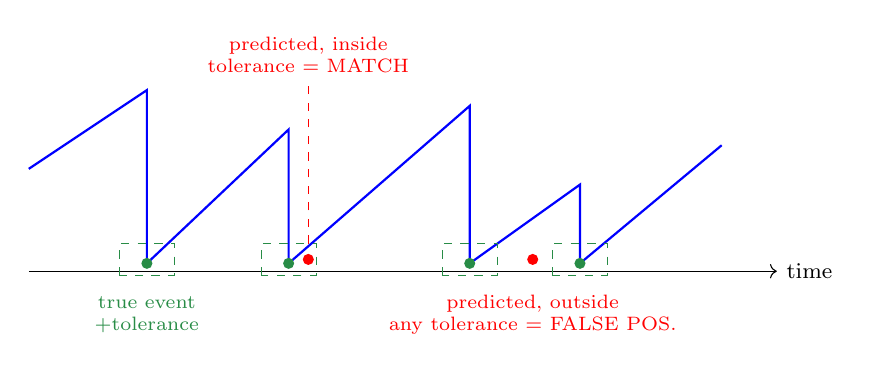
\begin{tikzpicture}
  \draw[->] (0,0) -- (9.5,0) node[right]{\footnotesize time};
  \draw[blue, thick] (0,1.3) -- (1.5,2.3) -- (1.5,0.1) -- (3.3,1.8) -- (3.3,0.1) -- (5.6,2.1) -- (5.6,0.1) -- (7,1.1) -- (7,0.1) -- (8.8,1.6);
  \foreach \x in {1.5,3.3,5.6,7} {
    \fill[okline] (\x,0.1) circle (2pt);
    \pgfmathsetmacro{\xlo}{\x-0.35}
    \pgfmathsetmacro{\xhi}{\x+0.35}
    \draw[okline, dashed] (\xlo,-0.05) rectangle (\xhi,0.35);
  }
  \node[okline, font=\scriptsize, align=center] at (1.5,-0.55) {true event\\+tolerance};
  \fill[red] (3.55,0.15) circle (2pt);
  \draw[red, thin, dashed] (3.55,0.35) -- (3.55,2.45);
  \node[red, font=\scriptsize, align=center, text width=3.0cm] at (3.55,2.75) {predicted, inside tolerance = MATCH};
  \fill[red] (6.4,0.15) circle (2pt);
  \node[red, font=\scriptsize, align=center] at (6.4,-0.55) {predicted, outside\\any tolerance = FALSE POS.};
\end{tikzpicture}
\caption{Event decoding and adaptive-tolerance matching: this is what scoring with \texttt{'f1'} actually checks -- timing agreement at the resets, not point-by-point curve similarity.}
\label{fig:event-matching}
\end{figure}

\subsection{Algorithm: \texttt{\_score} -- the shared dispatcher}
A single function every \texttt{proper\_*} routine calls internally (and this pipeline's own scoring functions call directly, e.g.\ \texttt{evaluate\_smap\_candidate}, \texttt{gmn\_fidelity\_rho}): given observed and predicted arrays and a metric name, route to Pearson correlation, mean absolute error, the event-F1 above, or the Kistler coincidence factor $\Gamma$ (an alternative, chance-corrected event-timing metric: matches events greedily nearest-pair-first within a fixed coincidence window \texttt{GAMMA\_DELTA}, then compares the match count against what a Poisson process at the same predicted rate would produce by chance -- $\Gamma{=}1$ perfect, $\Gamma{=}0$ chance-level).

\subsection{Design: \texttt{\_metric\_for} and the \texttt{TARGET\_METRIC}/\texttt{METRIC} split}
\label{sec:target-metric}
\begin{steps}
\item Given a column name and the list of behavioral targets, return \texttt{TARGET\_METRIC} (always \texttt{'correlation'}) if that column \emph{is} a target; otherwise return \texttt{METRIC} (\texttt{'f1'} by default).
\item Called at every scoring site that might be asked to score \emph{either} kind of column -- the interaction matrix (both sides of every pair independently), node-dimension estimation, and every post-hoc fidelity/forecast score.
\end{steps}
\pitfallbox{This distinction is not cosmetic -- see Section~\ref{sec:history-metric-bug}:}{Applying event-decoding metrics to a continuous behavioral trace is close to meaningless: \texttt{infer\_near\_zero\_threshold\_from\_true\_tsls} has nothing principled to lock onto on a signal with no genuine reset structure, and in one production run this produced silent \texttt{NaN} for every candidate in an $(E,\tau)$ grid search, crashing hours later at an unrelated step. Any future scoring call site \textbf{must} route through \texttt{\_metric\_for} rather than hardcoding \texttt{METRIC}.}

\newpage
% =====================================================================
\section{\texttt{MODE='GMN'}: The Original Interaction-Matrix Path}
\label{sec:gmn-mode}
% =====================================================================
Set \texttt{MODE='GMN'} to skip MDE selection entirely and build the network from the full, \texttt{REGION\_CHANNEL\_CAP}-limited candidate pool directly -- unaffected by the two-stage redesign above, and the one place this pipeline still needs a shared, network-wide $(E,\tau)$.

\begin{steps}
\item \texttt{target\_E\_tau\_rho\_grid}: split library data 70/30; for every $(E,\tau)$ in \texttt{E\_RANGE}$\times$\texttt{TAU\_RANGE}, run a univariate Simplex self-prediction of each target, scored via \texttt{TARGET\_METRIC}; average across targets, take the single best $(E,\tau)$ as the shared embedding for the whole interaction matrix.
\item \texttt{build\_interaction\_matrix}: for every unordered node pair, run \texttt{proper\_ccm} once (getting both directions), gate each with the convergence test (Section~\ref{sec:convergence-gate}), and record the passing direction's score at the largest library size -- \texttt{cleaned\_helper\_functions.proper\_ccm} in place of the sibling pipeline's \texttt{apps.InteractionMatrix} CLI subprocess.
\item \texttt{estimate\_node\_dimension}: per node, a univariate embedding-dimension sweep via \texttt{proper\_embed\_dimension}, used to cap each node's own driver count before \texttt{apps.CreateNetwork}'s greedy, acyclic BFS assembly (unmodified third-party code, same acyclicity guarantee as Stage 1's own eager cycle-rejection).
\end{steps}
\decisionbox{Why \texttt{proper\_ccm} has no pool-nesting concern, unlike the sibling pipeline's own \texttt{MODE='GMN'} path:}{The sibling pipeline's own interaction-matrix construction still shells out to \texttt{apps.InteractionMatrix}, whose outer pool is sized by \texttt{MDE\_GMN\_INTERACTION\_MATRIX\_OUTER\_CORES} against the same nested-pool-blowup risk described in Section~\ref{sec:history-pool}. \texttt{proper\_ccm} has no multiprocessing pool of its own at all (confirmed: no \texttt{Pool} usage anywhere in \texttt{cleaned\_helper\_functions.py}) -- there is nothing for an equivalent knob to size, so none is exposed here.}

\newpage
% =====================================================================
\section{Cross-Job Search Reuse and the Fingerprinting Architecture}
\label{sec:reuse}
% =====================================================================

\subsection{The problem: every expensive stage is deterministic, but resubmission used to redo it anyway}
MDE forward selection (Sections~\ref{sec:stage1}--\ref{sec:stage2}), network construction, theta search, and the generate-start sweep are each fully determined by their own inputs. A SLURM resubmission with identical settings -- common after a timeout on a multi-hour job -- used to pay for all of them again, for no reason.

\subsection{Algorithm: fingerprint-then-lookup, at four independent granularities}
\begin{steps}
\item Each stage builds its own fingerprint (\texttt{build\_mde\_selection\_fingerprint()}, \texttt{build\_multi\_mde\_selection\_fingerprint()}, \texttt{build\_network\_fingerprint()}, \texttt{build\_search\_fingerprint()}, \texttt{build\_start\_sweep\_fingerprint()}) -- every config knob that shapes that stage's outcome (including this pipeline's own \texttt{METRIC}/\texttt{TARGET\_METRIC}/\texttt{GAMMA\_DELTA}/\texttt{CCM\_WINDOW\_ROWS}/\texttt{CCM\_LIB\_SIZE\_PCTS}/\texttt{CCM\_SAMPLE}/\texttt{CCM\_SLOPE}, and \texttt{GMN\_MODE}/\texttt{MULTI\_MDE\_E}/\texttt{MULTI\_MDE\_TARGET\_AGGREGATE} (Section~\ref{sec:gmn-mode-joint}), folded in alongside the fields shared with the sibling pipeline), plus a hash of the input data file and a fingerprint of the pipeline's own code (\texttt{build\_code\_fingerprint()}, Section~\ref{sec:code-fingerprint}).
\item \texttt{find\_cached()} scans \texttt{TSLS\_MDE\_GMN\_PREV\_RUNS\_DIR} for a past job's matching cache file with an identical fingerprint.
\item A hit skips that stage's real work entirely and reconstructs its result from the cache; a miss just computes it normally -- always a safe, redundant-compute optimization, never a correctness shortcut, since a mismatch can never produce a false hit.
\end{steps}

\begin{figure}[H]
\centering
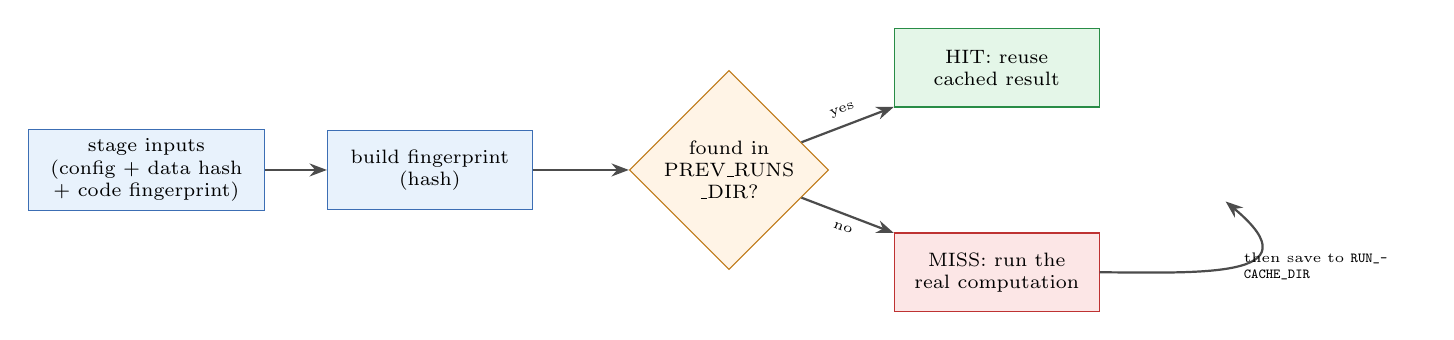
\begin{tikzpicture}[every node/.style={font=\scriptsize}]
  \node[rectangle, draw=stageline, fill=stagefill, minimum width=3cm, minimum height=1cm, align=center] (inputs) at (0,0) {stage inputs\\(config + data hash\\+ code fingerprint)};
  \node[rectangle, draw=stageline, fill=stagefill, minimum width=2.6cm, minimum height=1cm, align=center] (fp) at (3.6,0) {build fingerprint\\(hash)};
  \node[diamond, draw=stage2line, fill=stage2fill, minimum width=2.4cm, minimum height=1.6cm, align=center, inner sep=1pt] (lookup) at (7.4,0) {found in\\PREV\_RUNS\\\_DIR?};
  \node[rectangle, draw=okline, fill=okfill, minimum width=2.6cm, minimum height=1cm, align=center] (hit) at (10.8,1.3) {HIT: reuse\\cached result};
  \node[rectangle, draw=badline, fill=badfill, minimum width=2.6cm, minimum height=1cm, align=center] (miss) at (10.8,-1.3) {MISS: run the\\real computation};
  \draw[arrow] (inputs) -- (fp);
  \draw[arrow] (fp) -- (lookup);
  \draw[arrow] (lookup) -- (hit) node[midway, above, sloped, font=\tiny] {yes};
  \draw[arrow] (lookup) -- (miss) node[midway, below, sloped, font=\tiny] {no};
  \draw[arrow] (miss.east) .. controls +(1.2,0) and +(1.2,-1.0) .. ($(miss.east)+(1.6,0.9)$) node[midway, right, font=\tiny, text width=2.2cm] {then save to \texttt{RUN\_CACHE\_DIR}};
\end{tikzpicture}
\caption{The same fingerprint-then-lookup pattern, applied independently by MDE selection, network construction, theta search, and the start-point sweep -- a mismatched fingerprint can only ever fall through to MISS, never produce a false HIT.}
\label{fig:fingerprint-flow}
\end{figure}

Caching happens at full per-node granularity for MDE (\texttt{run\_mde\_for\_target()} is the single call site all three MDE call sites -- \texttt{main()}'s top-level seed, Stage 1, Stage 2 -- share), so a resubmission can resume node-by-node, not just stage-by-stage.

\subsection{\texttt{build\_code\_fingerprint} -- surviving a cosmetic edit}
\label{sec:code-fingerprint}
\texttt{\_strip\_docstrings()} parses the pipeline's own AST and removes every docstring before hashing, so a pure documentation edit does not invalidate every cache entry from every past job, while any change to actual logic still does. The hash covers \textbf{every module in the \texttt{mde\_gmn} package plus the calling entry script} (Section~\ref{sec:architecture}), so adding a module is tracked automatically and neither pipeline can reuse the other's cached results: the entry script's path is part of the input, which is why \texttt{main()} takes it as an argument rather than using its own \texttt{\_\_file\_\_}. \texttt{\_environment\_fingerprint()} additionally content-hashes \texttt{cleaned\_helper\_functions.py} itself -- there is no installed-package version to query for a local module, the same reasoning the sibling pipeline applies to \texttt{apps.CreateNetwork}/\texttt{apps.InteractionMatrix} -- and still tracks \texttt{gmn}'s own installed version, since Generate()/Forecast() still depend on it.

\linknote{Cached artifacts need somewhere durable to live -- Section~\ref{sec:storage} covers where.}

\newpage
% =====================================================================
\section{Cluster Storage Architecture}
\label{sec:storage}
% =====================================================================

\subsection{Four locations, three different lifetimes}
\begin{figure}[h]
\centering
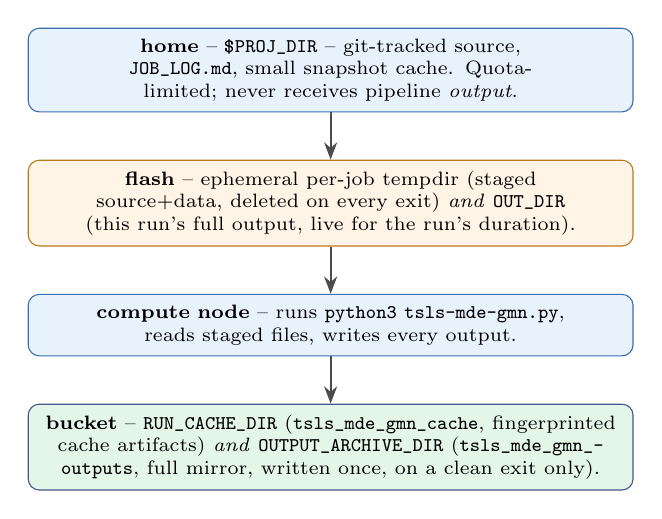
\begin{tikzpicture}[node distance=6mm, every node/.style={font=\scriptsize}]
  \node[smallbox, text width=7.4cm, draw=stageline] (home) {\textbf{home} -- \texttt{\$PROJ\_DIR} -- git-tracked source, \texttt{JOB\_LOG.md}, small snapshot cache. Quota-limited; never receives pipeline \emph{output}.};
  \node[smallbox, text width=7.4cm, below=of home, draw=flashline, fill=stage2fill] (flash) {\textbf{flash} -- ephemeral per-job tempdir (staged source+data, deleted on every exit) \emph{and} \texttt{OUT\_DIR} (this run's full output, live for the run's duration).};
  \node[smallbox, text width=7.4cm, below=of flash, draw=stageline] (compute) {\textbf{compute node} -- runs \texttt{python3 tsls-mde-gmn.py}, reads staged files, writes every output.};
  \node[smallbox, text width=7.4cm, below=of compute, draw=bucketline, fill=okfill] (bucket) {\textbf{bucket} -- \texttt{RUN\_CACHE\_DIR} (\texttt{tsls\_mde\_gmn\_cache}, fingerprinted cache artifacts) \emph{and} \texttt{OUTPUT\_ARCHIVE\_DIR} (\texttt{tsls\_mde\_gmn\_outputs}, full mirror, written once, on a clean exit only).};
  \draw[arrow] (home) -- (flash);
  \draw[arrow] (flash) -- (compute);
  \draw[arrow] (compute) -- (bucket);
\end{tikzpicture}
\caption{The four storage locations this pipeline touches -- a separate bucket namespace from the sibling pipeline's own \texttt{simple\_mde\_gmn\_cache}/\texttt{simple\_mde\_gmn\_outputs} pools, so the two pipelines' caches and archives never collide.}
\label{fig:storage}
\end{figure}

\subsection{The job-end fork: archive on success, preserve in place on failure}
\begin{steps}
\item The sbatch script captures \texttt{python3 tsls-mde-gmn.py}'s own exit status (\texttt{PY\_STATUS}) around a deliberate \texttt{set +e}/\texttt{set -e} pair -- necessary because the script otherwise runs under \texttt{set -euo pipefail}, which would jump straight to the exit trap on a nonzero exit without ever reaching the line that captures it.
\item The \texttt{cleanup} \texttt{EXIT} trap checks \texttt{PY\_STATUS}: \texttt{"0"} means the run completed cleanly, so \texttt{OUT\_DIR} is copied in full to \texttt{OUTPUT\_ARCHIVE\_DIR} (bucket) and the flash copy is then deleted.
\item Any other value -- a crash, a SLURM time-limit kill, a cancellation -- leaves \texttt{OUT\_DIR} exactly where it is on flash, untouched, for direct inspection (Section~\ref{sec:history-stage1-cost} is a real example of exactly this state).
\end{steps}
\decisionbox{Why this fork exists, not just "always archive" or "always keep on flash":}{Flash is meant to be genuine scratch, not permanent storage, once bucket has the headroom to be the durable copy -- but a failed run's partial output is exactly the case where fast, directly-browsable storage is most useful, so failure is deliberately excluded from the archive-and-clear path.}

\newpage
% =====================================================================
\section{The Progress-Monitoring Log}
\label{sec:progress-log}
% =====================================================================

\subsection{The problem: hours of real work with zero timing signal}
Runs under the current architecture have historically failed to finish even at generous walltimes while still doing genuine work the whole time (Section~\ref{sec:history-stage1-cost}: job 38976891 ran over three hours on a single depth-1 wave of just 3 nodes, nine worker processes confirmed alive and busy throughout, producing no new output the entire time). Before this feature, there was \textbf{no timing instrumentation anywhere in this codebase} -- zero uses of \texttt{time.perf\_counter()}/\texttt{datetime} in either pipeline file, and no duration was ever computed or logged. The only "progress" signal was a handful of untimestamped \texttt{print()} stage markers -- no notion of how long anything took, or was expected to take, and no explicit record of \emph{how} a job ended if it didn't finish cleanly.

\subsection{Where it lives, and why}
\texttt{cfg['RESULTS\_DIR'] / 'progress.log'} -- the same \texttt{OUT\_DIR} on \texttt{/flash} every other output already lives in (Section~\ref{sec:storage}), so this satisfies "save in flash" using the existing convention with no new path plumbing. Opened once in truncate mode at the very top of \texttt{main()}. Every write goes through one small helper:
\begin{steps}
\item \texttt{\_log\_progress(log\_path, message)}: appends one \texttt{datetime.now().isoformat()}-prefixed line, then \texttt{flush()} and \texttt{os.fsync()} \emph{immediately} -- so a line survives a crash the instant after it's written, not only on a clean close. \texttt{log\_path=None} is a silent no-op (every function that logs takes this as an optional keyword, so no existing call site or test that doesn't pass one is affected).
\item Called only from the main process -- worker processes (Stage 1/2's own \texttt{ProcessPoolExecutor}s, Section~\ref{sec:stage1-parallelization}) are never given this path, so there is no cross-process write contention to reason about.
\end{steps}

\subsection{What gets timed}
Every major step in \texttt{main()}'s own call order gets a START/END line with duration: the depth-0 MDE seed (both \texttt{GMN\_MODE} branches), \texttt{build\_network()} (including a start/end pair around GMN-mode network construction specifically), the theta search, the generate-start sweep, the final rebuild, the \texttt{Forecast()} diagnostic, \S\ref{sec:diagnostics}'s R7 diagnostics, and \texttt{run\_mde\_evaluate()} (or, when \texttt{RUN\_MDE\_EVALUATE=false}, the one-line skip notice, Section~\ref{sec:mde-evaluate-toggle}) -- table-stakes coverage of "every step," not just the historically slow ones.

\textbf{Stage 1 and Stage 2's own per-wave loops (Section~\ref{sec:stage1-algo}) get the fullest treatment}, since they are the confirmed historical bottleneck: every node gets its own START/END/duration line, and the blocking \texttt{for fut in as\_completed(futures):} pattern is replaced with a polling loop --
\texttt{concurrent.futures.wait(pending, timeout=HEARTBEAT\_SECONDS, return\_when=FIRST\_COMPLETED)}, \texttt{HEARTBEAT\_SECONDS=300} -- so a wave that is still genuinely working, but has completed nothing new in the last 5 minutes, writes a heartbeat line (nodes done so far, which nodes are still outstanding, elapsed time, current ETA) instead of going silent the way job 38976891's own multi-hour wave did.

\begin{figure}[h]
\centering
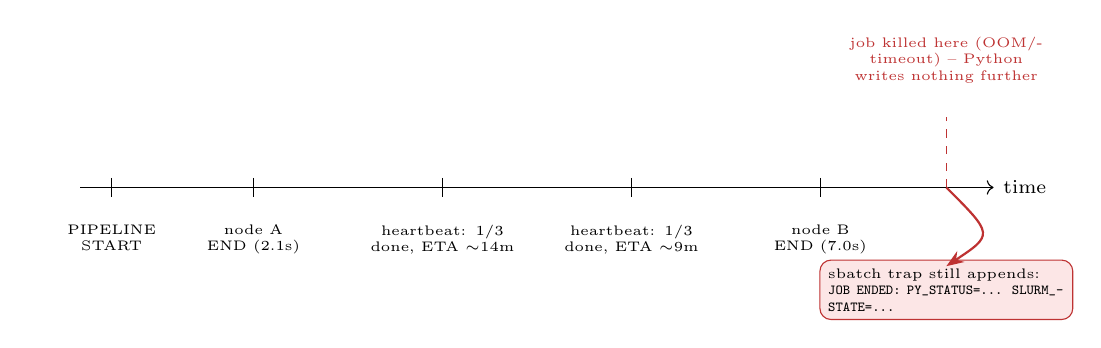
\begin{tikzpicture}[every node/.style={font=\scriptsize}, node distance=4mm]
  \draw[->] (0,0) -- (11.6,0) node[right]{time};
  \foreach \x/\lab in {0.4/{PIPELINE START}, 2.2/{node A END (2.1s)}, 4.6/{heartbeat: 1/3 done, ETA $\sim$14m}, 7.0/{heartbeat: 1/3 done, ETA $\sim$9m}, 9.4/{node B END (7.0s)}}
    { \draw (\x,0.12) -- (\x,-0.12); \node[below, font=\tiny, align=center, text width=1.9cm] at (\x,-0.35) {\lab}; }
  \node[above, badline, font=\tiny, align=center, text width=2.6cm] at (11.0,1.2) {job killed here (OOM/timeout) -- Python writes nothing further};
  \draw[dashed, badline] (11.0,0) -- (11.0,0.9);
  \node[draw=badline, fill=badfill, rounded corners, font=\tiny, align=left, text width=3.0cm, inner sep=3pt] at (11.0,-1.3) {sbatch trap still appends:\\\texttt{JOB ENDED: PY\_STATUS=... SLURM\_STATE=...}};
  \draw[arrow, badline] (11.0,0) .. controls (11.6,-0.6) .. (11.0,-1.0);
\end{tikzpicture}
\caption{A run's own timeline in \texttt{progress.log}: per-node START/END lines, heartbeats during a still-working wave, and -- even after a hard kill leaves Python unable to write anything further -- one last line appended by the sbatch script's own \texttt{cleanup} trap, querying SLURM's own authoritative exit state.}
\label{fig:progress-log-timeline}
\end{figure}

\subsection{ETA: based on this run's own completed work, never cross-job}
\texttt{\_format\_eta(durations, n\_remaining, per\_unit=None, unit\_remaining=None)} prefers a \textbf{per-window-row rate} (seconds per resolved ranking-window row, Section~\ref{sec:window-sizing}) over a flat per-node average whenever both are available -- a flat average is a weak estimate given real resolved windows range from a few hundred to \texttt{MAX\_WINDOW\_ROWS}'s own 30{,}000-row ceiling. Before submitting each pending node, \texttt{\_preview\_window\_rows()} speculatively, read-only resolves that node's own expected window size (reusing \texttt{\_resolve\_target\_ranking\_window()}'s own machinery purely for a size estimate, short-circuiting before touching real data for a behavioral target the same way the real resolve does) -- so the ETA scales by each still-pending node's own expected cost, not a uniform per-node guess. Every duration this feeds on comes only from steps \emph{already completed within this same run} -- never a cross-job average, which would conflate this run's own actual data/configuration with an unrelated past job's.

\subsection{Crash/timeout/OOM-safe final-state logging: the one piece that has to live outside Python}
A hard kill (SLURM time-limit \texttt{SIGTERM}/\texttt{SIGKILL}, an OOM-killer \texttt{SIGKILL}) means Python never gets a chance to write anything of its own past that point -- no exception handler, no \texttt{finally} block runs. The sbatch script's own \texttt{cleanup} \texttt{EXIT} trap is extended with \texttt{log\_final\_outcome()}: it queries \texttt{sacct -j "\$SLURM\_JOB\_ID" --format=State -P -n} -- SLURM's own authoritative record, able to distinguish \texttt{TIMEOUT}/\texttt{OUT\_OF\_MEMORY}/\texttt{CANCELLED}/\texttt{FAILED}/\texttt{COMPLETED}, which a raw \texttt{\$?} alone cannot -- retried a few times with a short sleep (since \texttt{sacct}'s own record can lag briefly right at trap time), and appends one final line to \texttt{progress.log} (if it exists): \texttt{JOB ENDED: PY\_STATUS=<n> SLURM\_STATE=<state>}.
\pitfallbox{The retry window was found insufficient on a real crash, not just in theory:}{A real job's own trap recorded \texttt{SLURM\_STATE=RUNNING} instead of the job's actual final state, because \texttt{sacct} had not yet updated within the original 3-attempt/2-second-sleep window -- job-end state is genuinely unreliable immediately at exit, not merely as a defensive assumption. A wider retry window has been proposed but was, at the time of writing, not yet implemented in the trap itself -- treat \texttt{SLURM\_STATE=RUNNING} in an already-exited job's own \texttt{progress.log} as a known artifact of this gap, not a contradiction, and cross-check with a fresh \texttt{sacct -j <job\_id>} query run \emph{after} the job has fully exited rather than trusting the trap's own snapshot alone.}
\pitfallbox{Honest limitation, stated up front rather than hidden:}{A genuinely instantaneous whole-cgroup \texttt{SIGKILL} (rare, but possible under some OOM-killer configurations) can in principle prevent even the trap itself from running. \texttt{sacct -j <job\_id>}, queried independently from outside the job after it has exited, remains the authoritative fallback in that case regardless of what \texttt{progress.log} itself managed to capture.}

\newpage
% =====================================================================
\section{End-to-End Data Flow}
\label{sec:e2e}
% =====================================================================

\begin{figure}[h]
\centering
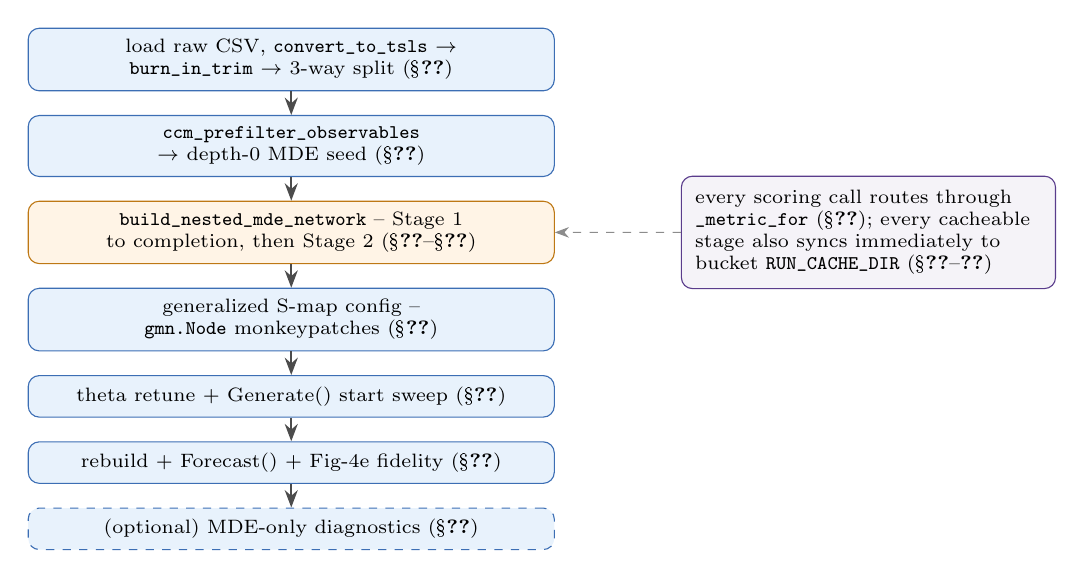
\begin{tikzpicture}[scale=0.85, every node/.style={font=\scriptsize}, node distance=3mm]
  \node[smallbox, text width=6.4cm] (load) {load raw CSV, \texttt{convert\_to\_tsls} $\to$ \texttt{burn\_in\_trim} $\to$ 3-way split (\S\ref{sec:split})};
  \node[smallbox, text width=6.4cm, below=of load] (pre) {\texttt{ccm\_prefilter\_observables} $\to$ depth-0 MDE seed (\S\ref{sec:gmn-mode-joint})};
  \node[smallbox, text width=6.4cm, below=of pre, fill=stage2fill, draw=stage2line] (s1) {\texttt{build\_nested\_mde\_network} -- Stage 1 to completion, then Stage 2 (\S\ref{sec:stage1}--\S\ref{sec:stage2})};
  \node[smallbox, text width=6.4cm, below=of s1] (smap) {generalized S-map config -- \texttt{gmn.Node} monkeypatches (\S\ref{sec:smap})};
  \node[smallbox, text width=6.4cm, below=of smap] (search) {theta retune + Generate() start sweep (\S\ref{sec:search})};
  \node[smallbox, text width=6.4cm, below=of search] (validate) {rebuild + Forecast() + Fig-4e fidelity (\S\ref{sec:validation})};
  \node[smallbox, text width=6.4cm, below=of validate, dashed] (diag) {(optional) MDE-only diagnostics (\S\ref{sec:diagnostics})};
  \foreach \a/\b in {load/pre,pre/s1,s1/smap,smap/search,search/validate,validate/diag}
    \draw[arrow] (\a) -- (\b);
  \node[right=1.6cm of s1, text width=4.4cm, draw=linknote, fill=linknote!6, rounded corners, inner sep=5pt] (sidenote) {every scoring call routes through \texttt{\_metric\_for} (\S\ref{sec:target-metric}); every cacheable stage also syncs immediately to bucket \texttt{RUN\_CACHE\_DIR} (\S\ref{sec:reuse}--\ref{sec:storage})};
  \draw[faintarrow] (sidenote.west) -- (s1.east);
\end{tikzpicture}
\caption{Full pipeline data flow, \texttt{main()}'s actual call order.}
\label{fig:e2e}
\end{figure}

\newpage
% =====================================================================
\section{Actual Outputs: Real Runs of This Codebase}
\label{sec:outputs}
% =====================================================================

\subsection{What these runs were, honestly}
This redesign has not yet completed a full SLURM job end-to-end at the time of writing. Three separate, genuinely real runs of the current codebase are reported below instead, each honestly labeled with what it does and does not demonstrate -- consistent with this document's own policy of reporting real, if incomplete, evidence rather than a hypothetical clean result.
\begin{itemize}
  \item \textbf{Interactive validation run A} (real data, \texttt{J1620210605\_epoch\_8\_freq\_40\_Hz.csv}, 47{,}999 raw rows, \texttt{REGION\_CHANNEL\_CAP=3}, \texttt{MDE\_D=2}, \texttt{METRIC=correlation} for this run specifically): completed Stage 1's full BFS and Stage 2's lag attachment for both targets, and began theta retuning for the resulting combined network, before its own log was cut off by an unrelated scratchpad-lifecycle event (not a pipeline bug -- Section~\ref{sec:history-stage1-cost}'s own honesty policy applies equally here: this is reported as an inconclusive tail, not papered over).
  \item \textbf{Interactive validation run B} (small synthetic dataset, 6{,}000 rows, same \texttt{REGION\_CHANNEL\_CAP=3}/\texttt{MDE\_D=2}): completed the \emph{entire} pipeline end-to-end -- MDE selection, theta search, \texttt{Generate()} fidelity, a \texttt{Forecast()} diagnostic guard rejection, and printed \texttt{"Pipeline complete"}.
  \item \textbf{SLURM calibration job 38976891} (real data, \texttt{REGION\_CHANNEL\_CAP=15}, \texttt{MDE\_D=4}, \texttt{NESTED\_M=1}, \texttt{GENERATE\_LENGTH=100}): the first real cluster submission of this exact codebase. Still in progress at the time of writing -- Section~\ref{sec:history-stage1-cost} reports its real, concerning performance profile.
\end{itemize}

\subsection{Run A: real Stage 1 + Stage 2 selections}
For \texttt{head\_position\_x}, Stage 1 selected two real drivers at depth 0: \texttt{OFC\_2\_tsls}, \texttt{OFC\_1\_tsls}. For \texttt{head\_position\_y}, Stage 1 selected \textbf{zero} real drivers at depth 0 -- a real, reported-not-hidden result (the same honest-reporting policy Section~\ref{sec:outputs} of the sibling document applies to its own small-scale MDE-vs-baseline result). Stage 2 then attached, for \texttt{head\_position\_x}: \texttt{CA1\_2\_tsls::delay-9}, \texttt{OFC\_1\_tsls::delay-1/-3/-5/-7/-9}, \texttt{CA1\_2\_tsls::delay-1/-3/-5/-7} (10 lagged edges); for \texttt{head\_position\_y}: \texttt{CA1\_1\_tsls::delay-7}, \texttt{mPFC\_0\_tsls::delay-7/-9}, \texttt{mPFC\_2\_tsls::delay-7}, \texttt{OFC\_2\_tsls::delay-3}, \texttt{OFC\_1\_tsls::delay-1/-3} (7 lagged edges) -- confirming Stage 2's own whole-universe search (Section~\ref{sec:stage2}) reaches real drivers even for a target that found none of its own at depth 0. Final parent lists: \texttt{head\_position\_x} $\leftarrow$ \{\texttt{OFC\_2\_tsls}, \texttt{OFC\_1\_tsls}, \texttt{CA1\_2\_tsls}\}; \texttt{head\_position\_y} $\leftarrow$ \{\texttt{CA1\_1\_tsls}, \texttt{mPFC\_0\_tsls}, \texttt{mPFC\_2\_tsls}, \texttt{OFC\_2\_tsls}, \texttt{OFC\_1\_tsls}\}. Theta retuning then began for the resulting combined 11-node network.

\subsection{Run B: a complete pipeline pass, including a real \texttt{Forecast()} guard rejection}
Run B's theta search reached a real score of \textbf{0.9827} for its combined network, then computed \texttt{Generate()} fidelity per node. Its \texttt{Forecast()} diagnostic then hit a real, legitimate validation failure -- reported verbatim, since this is exactly the kind of fail-fast guard Section~\ref{sec:split}'s own leakage machinery is designed to produce rather than a silent wrong answer:
\begin{center}
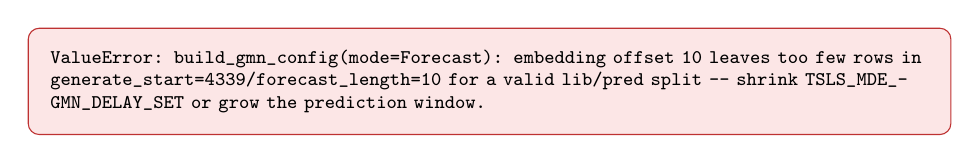
\begin{tikzpicture}
\node[draw=badline, fill=badfill, rounded corners, text width=0.92\linewidth, inner sep=8pt, align=left, font=\scriptsize\ttfamily]
{ValueError: build\_gmn\_config(mode=Forecast): embedding offset 10 leaves too few rows in generate\_start=4339/forecast\_length=10 for a valid lib/pred split -- shrink TSLS\_MDE\_GMN\_DELAY\_SET or grow the prediction window.};
\end{tikzpicture}
\end{center}
This is \texttt{build\_gmn\_config}'s own Forecast-mode row-index guard (Section~\ref{sec:smap}'s discussion of the embedding-offset shift) correctly refusing to run rather than silently truncating or crashing with a cryptic index error -- caught cleanly, logged, and skipped for this network's plot/rho only (Generate()-based outputs are unaffected, per this pipeline's own exception-guarding policy, Section~\ref{sec:stage1}). The run finished, printing \texttt{"Pipeline complete"} -- the first genuine, unbroken, end-to-end pass of the redesigned architecture on this codebase.

\subsection{Stage 1 diagnostics from the in-progress SLURM calibration job}
\begin{figure}[H]
\centering
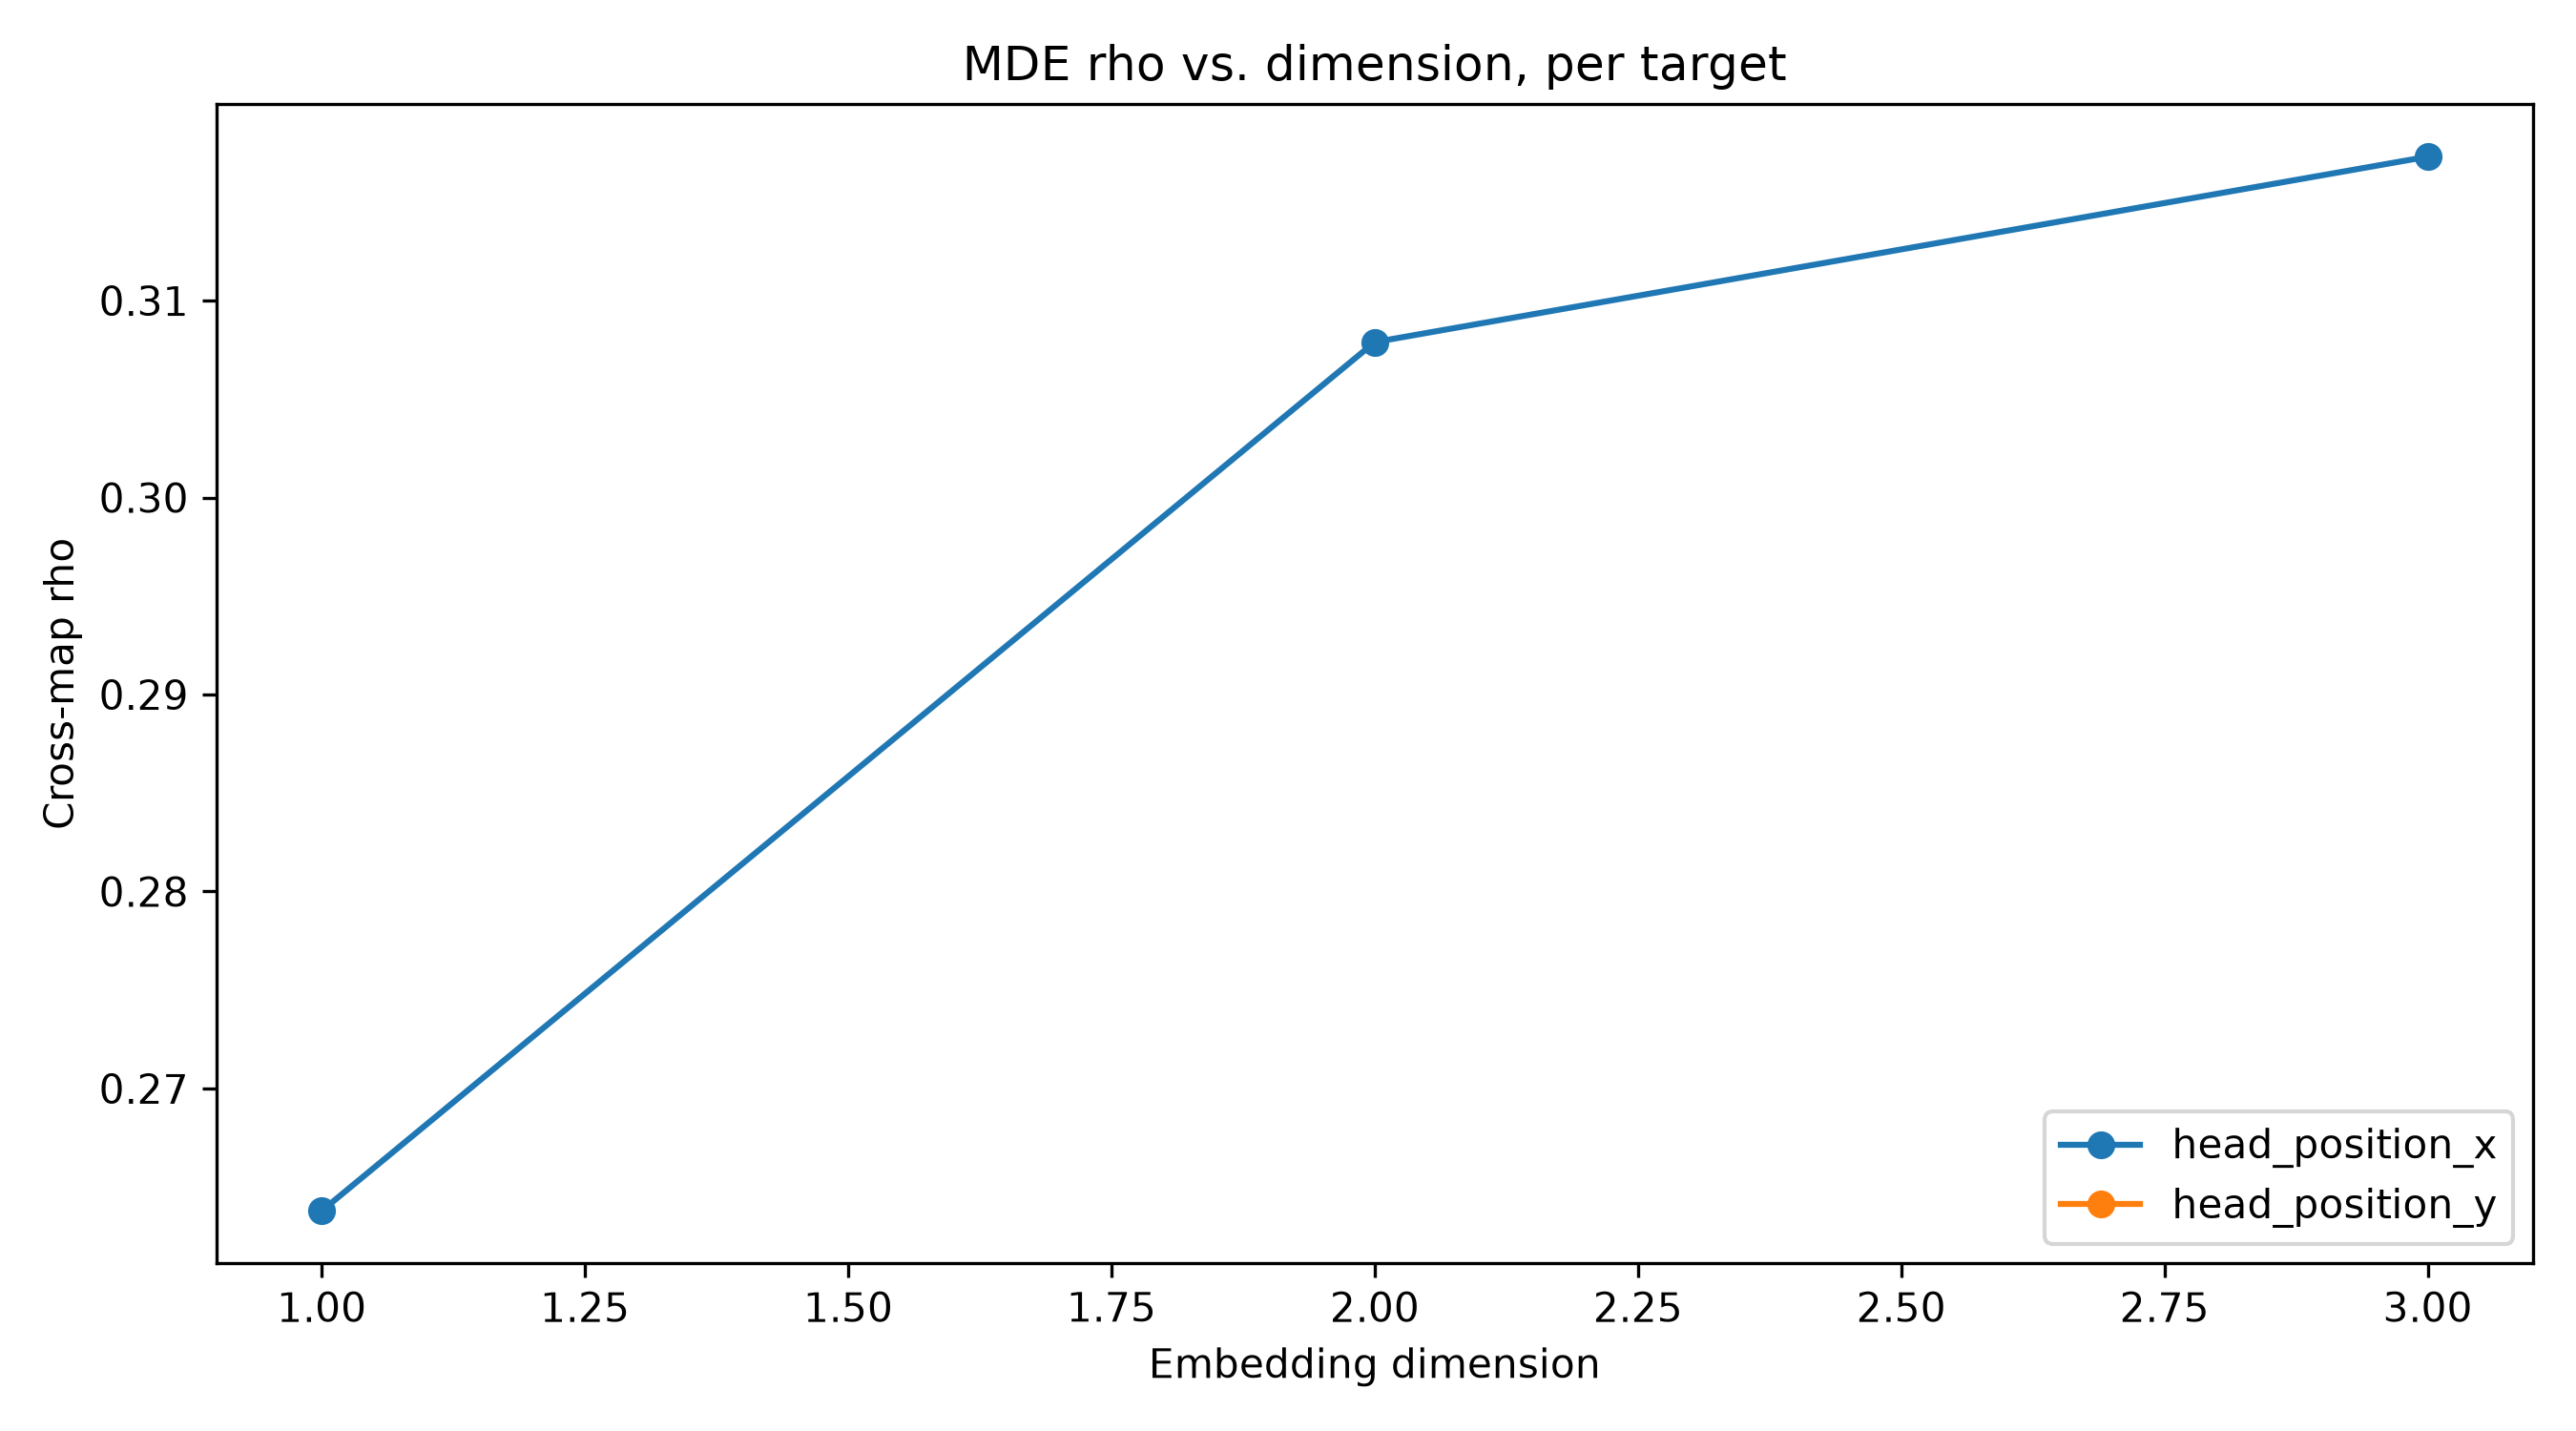
\includegraphics[width=0.72\textwidth]{figures/tsls_mde_rho_vs_dimension_multi_target.png}
\caption{Real \texttt{plot\_mde\_rho\_vs\_dimension()} output from job 38976891's depth-0 MDE call. \texttt{head\_position\_x} (blue) reaches dimension 3 with cross-map rho climbing $\approx$0.264 $\to$ 0.308 $\to$ 0.317 -- the expected diminishing-but-positive-returns shape. \texttt{head\_position\_y} (orange, no visible line) selected \textbf{zero} real drivers at this \texttt{REGION\_CHANNEL\_CAP=15}/\texttt{MDE\_D=4} scale -- reported honestly rather than omitted, consistent with Run A's own smaller-scale result above.}
\label{fig:rho-vs-dim}
\end{figure}

\begin{figure}[H]
\centering
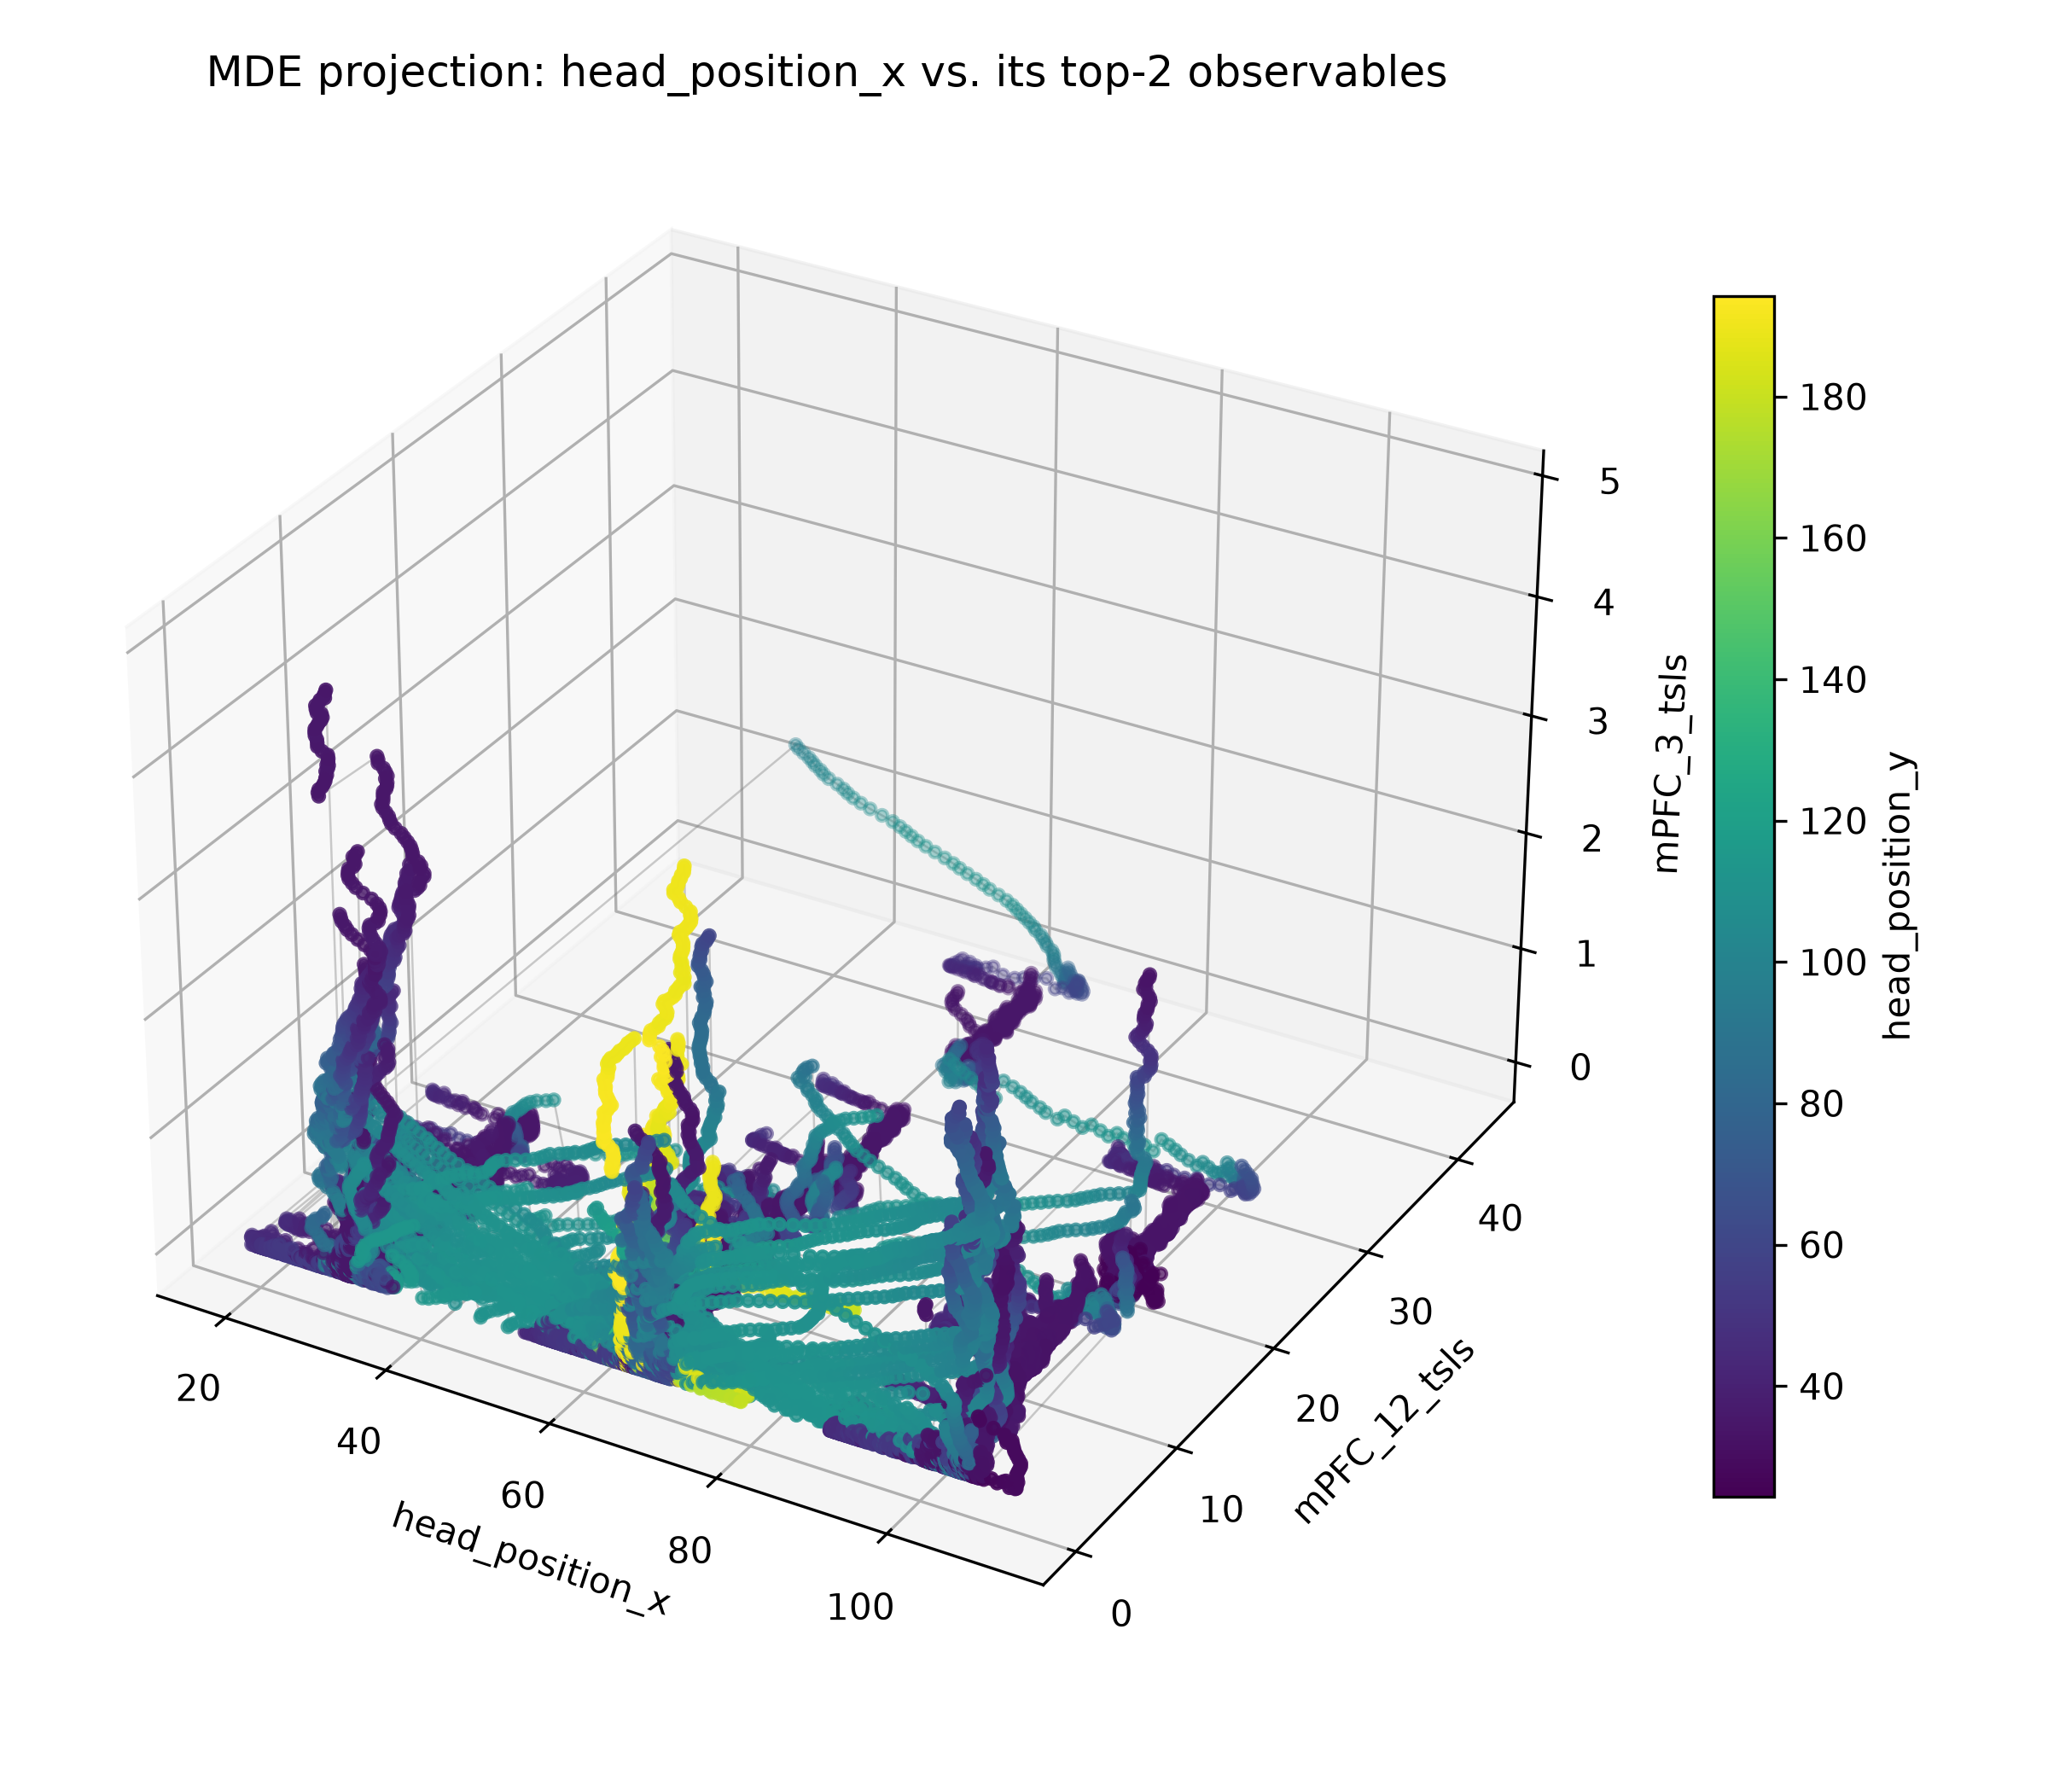
\includegraphics[width=0.62\textwidth]{figures/tsls_mde_3d_projection_head_position_x.png}
\caption{Real \texttt{plot\_3d\_mde\_projection()} output from job 38976891: \texttt{head\_position\_x} against its own top-2 depth-0 drivers (\texttt{mPFC\_12\_tsls}, \texttt{mPFC\_3\_tsls}), colored by \texttt{head\_position\_y}. All three of \texttt{head\_position\_x}'s depth-0 drivers (\texttt{mPFC\_12}/\texttt{mPFC\_3}/\texttt{mPFC\_9\_tsls}) had already become their own depth-1 nested-MDE targets by the time this figure was written, confirming Stage 1's BFS genuinely recursed at this scale (Section~\ref{sec:stage1}).}
\label{fig:3d-projection}
\end{figure}

\newpage
% =====================================================================
\section{Development History: Challenges, Investigations, and Design Decisions}
\label{sec:history}
% =====================================================================
Written for a reviewer, not a user: for every major issue, the observed symptom, what was actually wrong, the decision made, and the risk that decision leaves open. Entries are grouped chronologically into this pipeline's original TSLS-specific engineering, then the more recent two-stage architectural port.

\subsection{Missing dependency path (immediate, deterministic failure)}
\textbf{Symptom:} the very first job submission for this pipeline would fail within seconds, before any real computation.\\
\textbf{Cause:} the batch script's file-staging step referenced a nonexistent path; the actual helper file lived under \texttt{scripts/src/} instead.\\
\textbf{Decision:} corrected the staging path. No tradeoff -- a plain path error caught before any real job ran.

\subsection{The nested-multiprocessing-pool blowup}
\label{sec:history-pool}
\textbf{Symptom (in the sibling pipeline, historically, before either pipeline had its current design):} jobs ran roughly two days regardless of dataset size, mode, or parameter choice.\\
\textbf{Investigation:} process counts observed empirically (dozens of live processes from a single-digit core request); reading \texttt{pyEDM}'s installed source directly showed \texttt{CCM()} spawns a brand-new multiprocessing pool sized to the full visible core count on \emph{every single call}.\\
\textbf{Decision:} a monkeypatch forcing \texttt{pyEDM.CCM} onto its sequential in-process path, later folded into a venv-wide \texttt{sitecustomize.py} so it reaches subprocess-invoked tools too.\\
\textbf{Risk carried forward:} when this pipeline was first ported from the sibling's design, this specific patch had to be manually re-applied and was, for a time, simply absent -- caught in review before a full-scale run. This patch must still be manually kept in sync between the two pipelines; it is duplicated code, not shared.

\subsection{Cross-pipeline log contamination}
\textbf{Symptom:} a shared job-logging script's "compare this job against the most recent earlier job" logic had no way to distinguish which \emph{pipeline} an earlier job belonged to.\\
\textbf{Decision:} derive snapshot filenames (and the "most recent job" search) from the actual source filenames passed in, per invocation, instead of a hard-coded name. No tradeoff.

\subsection{The empty-network investigation}
\label{sec:history-interaction-bug}
\textbf{Symptom:} the constructed GMN network repeatedly came out with either zero nodes, or all targets present but no driver edges at all.\\
\textbf{Hypothesis 1 (rejected): under-parameterization.} Widened every relevant parameter; still empty -- ruled out.\\
\textbf{Hypothesis 2 (partially right, insufficient): a collapsed single-point search grid.} Widened; still empty -- a real contributing risk, not the root cause.\\
\textbf{Hypothesis 3 (confirmed): the convergence gate's library-size calibration.} A failed run's own interaction-matrix CSV was preserved and inspected directly: 88 of 90 off-diagonal cells at \emph{exactly} 0.0, not small or negative -- not a value real correlation produces by chance. The "small" library size in the convergence sweep was a fixed percentage of the \emph{entire} dataset, already well past where a real, low-dimensional relationship's cross-map skill saturates.\\
\textbf{Decision:} bound the row count fed into every percentage-based library-size sweep to a much smaller window (Section~\ref{sec:calibration}).

\subsection{The engine replacement: dimx.MDE $\to$ proper\_mde, and a metric-application bug it introduced}
\label{sec:history-tier}
\label{sec:history-metric-bug}
A methodological question was raised: correlation over a raw TSLS sawtooth is dominated by the smooth, uninformative ramp segments between spikes, not the informative resets -- shouldn't the pipeline score \emph{spike timing} directly? This led to the staged replacement of every \texttt{dimx}/\texttt{pyEDM}-direct call with a TSLS-aware equivalent from \texttt{cleaned\_helper\_functions.py} -- \texttt{proper\_mde} in place of \texttt{dimx.MDE}, documented throughout Section~\ref{sec:mde-engine} as the current design. This rewrite introduced its own bug:\\
\textbf{Symptom:} an $(E,\tau)$ grid search scoring a \emph{target}'s own self-predictability returned \texttt{NaN} for every candidate, crashing with an "all-NaN slice" error.\\
\textbf{Investigation:} traced to the event-decoding metric (\texttt{'f1'}) being applied uniformly, including to the two continuous behavioral targets, which have no genuine spike/reset structure to calibrate against.\\
\textbf{Decision:} introduced the \texttt{TARGET\_METRIC}/\texttt{METRIC} split and the \texttt{\_metric\_for} dispatcher (Section~\ref{sec:target-metric}).\\
\textbf{Risk carried forward:} only as strong as every future scoring call site remembering to route through \texttt{\_metric\_for} -- no type system or runtime check enforces this.

\subsection{A silently-swallowed exception}
\textbf{Symptom:} even after the metric-application bug above was fixed, the same $(E,\tau)$ grid search still returned all-\texttt{NaN}.\\
\textbf{Investigation:} the grid-search function wraps each candidate's Simplex call in a bare \texttt{try/except: pass}. Direct isolated testing surfaced a \texttt{TypeError}: a helper was still returning library/prediction ranges in \texttt{pyEDM}'s own \texttt{"start stop"} string format, but \texttt{proper\_simplex} expects a \texttt{[start, stop]} list.\\
\textbf{Decision:} fixed the helper to return the list form both call sites require.\\
\textbf{Risk carried forward:} the bare \texttt{try/except: pass} pattern that hid this bug is still present at several points (grid searches, per-pair CCM calls) -- deliberate, but it means a \emph{class} of bugs, not just expected numerical failures, can hide behind a silently-all-\texttt{NaN} result.

\subsection{Removing a validation gate versus recalibrating it}
\label{sec:history-noccm}
\textbf{Symptom:} after the fixes above, the CCM causality gate rejected \emph{every single candidate} for both targets, despite the ranking stage finding candidates with clearly non-trivial skill. The pipeline did not fail cleanly -- it ran for hours before crashing downstream.\\
\textbf{First response (later reverted): disable the gate.} \texttt{noCCM=True} made the pipeline run to completion, but on reflection was the wrong response: the CCM gate is the \emph{only} thing distinguishing correlation from causal drive, for a pipeline whose entire purpose is reporting causally-validated structure. Flagged in review and reverted before use in any real result.\\
\textbf{Experiment:} rather than argue from first principles, a handful of specific candidate pairs with strong ranking-stage scores were run through the raw CCM machinery at genuinely small library sizes (tens of rows), and the resulting skill-vs-library-size curve inspected by eye.\\
\textbf{Result:} a real, smooth, monotonically rising convergence curve appeared for the causally plausible direction, while the reverse direction stayed flat -- the textbook directional-asymmetry signature, absent in pure-noise control pairs tested the same way.\\
\textbf{Final decision:} the gate was restored, and \texttt{CCM\_WINDOW\_ROWS}/\texttt{CCM\_LIB\_SIZE\_PCTS} recalibrated so the smallest tested library falls inside the range where the real convergence signal was empirically confirmed (Section~\ref{sec:calibration}).
\pitfallbox{What a reviewer should still scrutinize:}{This investigation validated the calibration on a \emph{small number of hand-picked pairs}, not exhaustively across the full candidate pool, and showed real sensitivity to whether library draws span the full recording or a bounded contiguous window. Treat the current defaults as a validated starting point, not a proven-optimal calibration.}

\subsection{PCA-adjacent NaN warm-up rows}
\label{sec:history-pca}
\textbf{Symptom:} a downstream diagnostic died on delay-expansion warm-up rows reaching a NaN-intolerant consumer.\\
\textbf{Investigation:} \texttt{expand\_delay\_columns()} shifts each observable forward by $|{\rm delay}|$ rows, leaving that many leading rows \texttt{NaN}.\\
\textbf{Decision:} \texttt{run\_mde\_for\_target()} computes \texttt{warmup = max(|d|\ for\ d\ in\ delay\_set)} and starts \texttt{lib} at \texttt{warmup+1}, so every delay column is fully populated before any downstream consumer sees it (Section~\ref{sec:leakage-guard}).\\
\textbf{Risk carried forward:} found by a real crash, not by inspection -- any future new consumer of \texttt{mde\_df} that assumes zero \texttt{NaN} without checking this same warm-up convention could reintroduce an equivalent failure.

\subsection{The two-stage architectural port from simple-mde-gmn.py}
\label{sec:history-port}
\textbf{Context:} \texttt{simple-mde-gmn.py} independently underwent a major redesign (two-stage nested-MDE network construction, the leakage-safe three-way split, the generalized per-driver-delay embedding, exception-guarding, cross-job caching, the flash+bucket storage architecture) that this pipeline had not yet received -- confirmed via \texttt{git log}: the only commit touching either \texttt{tsls-mde-gmn.py} or its sbatch script predated all of that work.\\
\textbf{Decision:} rewrote both files from scratch, porting every one of the sibling's design changes, while keeping only what TSLS's own data representation and scoring genuinely require to differ (Section~\ref{sec:sibling}) -- \texttt{simple-mde-gmn.py}/\texttt{.sbatch} were not touched at all in the process (confirmed via \texttt{git diff --stat}).\\
\textbf{Verification performed before any cluster submission:} \texttt{python3 -m py\_compile} and \texttt{bash -n} both clean; systematic grep-based auditing confirmed zero live references to the dropped machinery (\texttt{dimx}, \texttt{apps.InteractionMatrix}, \texttt{subprocess}, \texttt{EmbedDimension(}, \texttt{PredictInterval(}, \texttt{ComputeError(}, \texttt{SMAP\_SEARCH\_MODE}); two interactive smoke tests against real data (Runs A and B, Section~\ref{sec:outputs}) exercised the entire pipeline before any SLURM submission.\\
\textbf{Risk carried forward:} no SLURM job under the new architecture has yet completed end-to-end (Section~\ref{sec:history-stage1-cost}) -- the interactive smoke tests validate correctness at small scale, not cluster-scale performance.

\subsection{A calibration run's own \texttt{GENERATE\_LENGTH} trap, caught before submission}
\label{sec:history-generate-length}
\textbf{Symptom (caught during review, not in production):} while sizing the first post-port calibration job's SLURM resources, \texttt{GENERATE\_LENGTH} had been left at its default (\texttt{0}, "use the full held-out window") while \texttt{REGION\_CHANNEL\_CAP}/\texttt{MDE\_D}/\texttt{NESTED\_M} were already set small for calibration.\\
\textbf{Investigation:} reading \texttt{derive\_lag\_set()} and \texttt{main()} directly showed \texttt{GENERATE\_LENGTH}'s \texttt{0} sentinel resolves to the \emph{full} held-out window (thousands of rows) \emph{before} \texttt{LAG\_MODE=generation\_length\_adjusted} uses it as Stage 2's lag-candidate bound -- so a "small" calibration run would have silently searched thousands of lag columns per real observable in Stage 2, defeating the entire purpose of the calibration scale-down.\\
\textbf{Decision:} set \texttt{GENERATE\_LENGTH=100} explicitly for calibration runs, tagged \texttt{VALIDATION RUN} in the sbatch script alongside \texttt{REGION\_CHANNEL\_CAP}/\texttt{MDE\_D}.\\
\textbf{Resolution (2026-10-01):} \texttt{DELAY\_SOURCE=tau\_count} (Section~\ref{sec:lag-set}) decouples the two quantities -- the lag count is stated as \texttt{LAG\_COUNT} and \texttt{GENERATE\_LENGTH} no longer bounds it.\\
\textbf{Risk carried forward:} on the default \texttt{lag\_mode} path the original trap is unchanged: a "small" run there must still cap \texttt{GENERATE\_LENGTH} explicitly, because it is not implied by capping the other three knobs. The new mode removes the coupling only for runs that opt into it.

\subsection{Stage 1's real cost at calibration scale, still open}
\label{sec:history-stage1-cost}
\textbf{Symptom:} job 38976891 (\texttt{REGION\_CHANNEL\_CAP=15}, \texttt{MDE\_D=4}, \texttt{NESTED\_M=1}, \texttt{GENERATE\_LENGTH=100} -- sized specifically to be a small, fast calibration run, Section~\ref{sec:outputs}) completed its depth-0 seed for both targets within the first two minutes, but its single depth-1 wave (3 nodes: \texttt{mPFC\_12\_tsls}, \texttt{mPFC\_3\_tsls}, \texttt{mPFC\_9\_tsls}) had not produced any new output files more than three hours later, against a 4-hour wall-clock budget.\\
\textbf{Investigation:} checked directly on the compute node (not merely inferred from the SLURM queue) -- nine worker processes were confirmed alive and consuming 90--105\% CPU each, continuously, for the entire elapsed time. This rules out a hang/deadlock: the job is doing real, sustained work, just far more of it than the interactive smoke tests (Runs A/B, at a smaller \texttt{REGION\_CHANNEL\_CAP=3}) predicted.\\
\textbf{Status at time of writing:} still running, real cause of the cost jump between \texttt{REGION\_CHANNEL\_CAP=3} and \texttt{REGION\_CHANNEL\_CAP=15} not yet isolated -- candidate pool size enters \texttt{proper\_mde}'s ranking stage roughly linearly per dimension, but has not been directly profiled at this scale.\\
\textbf{Decision:} reported here as an open finding rather than silently resubmitted with larger resources -- resubmitting without first understanding the cost driver risks masking a real inefficiency behind more compute, the same lesson the sibling pipeline's own resource-sizing history draws explicitly.\\
\textbf{Risk carried forward:} the sbatch script's own 4-hour calibration budget may be too tight even for this deliberately small a configuration; Section~\ref{sec:future} makes characterizing this cost curve a concrete next step.

\subsection{The \texttt{CA1\_12\_tsls} crash: two fixes made together}
\label{sec:history-prefilter-order}
\textbf{Symptom:} job 39605473 crashed 3m35s in with \texttt{ValueError: invalid literal for int() with base 10: 'CA1\_12\_tsls'}.\\
\textbf{Investigation:} the traceback led to \texttt{observable\_and\_delay()} $\to$ \texttt{\_parse\_delayed\_column\_name()}, which assumes any column name not found verbatim in \texttt{raw\_columns} must carry a \texttt{::delay-N} suffix to strip and parse -- but \texttt{CA1\_12\_tsls} carried no such suffix; it was simply absent from \texttt{raw\_columns}. The root cause: depth-0's own MDE seed, in \texttt{main()}, searched the \emph{full}, unfiltered observable pool, while the CCM pre-filter (Section~\ref{sec:ccm-prefilter}) only narrowed the pool \emph{afterward}, inside \texttt{build\_network()} -- so a depth-0-selected real observable could legitimately not exist in the smaller, filtered \texttt{raw\_columns} list that Stage 1/2's own BFS used (Section~\ref{sec:why-depth0-explicit}'s Figure~\ref{fig:prefilter-ordering} illustrates the mismatch directly). The sibling pipeline hit the identical bug the same way, on its own raw (non-\_tsls-suffixed) column names -- job 39605472 crashed on \texttt{'CA1\_22'} (sibling document, "The \texttt{CA1\_22} crash: two fixes made together"). A first patch, verified via resubmission (job 39655804), added a marker-presence fallback to \texttt{observable\_and\_delay()} so an unrecognized name is treated as a plain delay-0 observable rather than crashing -- this kept jobs running, but review found it papered over the mismatch rather than fixing it, alongside a second, unrelated design gap in how Stage 2's picks were represented, since redesigned entirely (Section~\ref{sec:stage2-leaves}).\\
\textbf{Decision (per explicit request, both fixes made together):} (1) \texttt{main()} now runs \texttt{ccm\_prefilter\_observables()} once per target group \emph{before} seeding depth-0, so depth-0 and every later nested-MDE round search the exact same filtered pool -- the mismatch this crash depended on can no longer occur on a normal run. (2) Stage 1 and Stage 2 were unified into one per-wave BFS (Section~\ref{sec:stage1}) so a Stage-2 real-observable pick recurses exactly like a Stage-1 one. Both were verified on real data locally (isolated probe calls confirmed Stage-2-style real-observable picks actually recurse, on both this pipeline's 40\,Hz data and the sibling pipeline's 1\,Hz data) before the next cluster submission (job 39671000).\\
\textbf{Risk carried forward:} the \texttt{observable\_and\_delay()} fallback was kept, not removed -- it is now a pure safety net for cross-job cache reuse (\texttt{REUSE\_BEST\_PARAMS}), where a reused \texttt{mde\_results} entry can legitimately come from an earlier job that used a different \texttt{CCM\_PREFILTER\_RHO\_MIN}/\texttt{CCM\_PREFILTER\_E}, or predates the pre-filter feature entirely, and so can still reference an observable absent from \emph{this} run's own filtered \texttt{raw\_columns}. A reviewer should not read its continued presence as evidence the ordering bug is still live on a normal (non-cache-reuse) run.

\subsection{The depth-$\ge$1 metric-routing bug: every neuron driver ranked by the wrong metric}
\label{sec:history-metric-routing}
\textbf{Symptom:} a verbose log line printed \texttt{(correlation=0.9997)} for a neuron node's own ranking-stage acceptance -- the wrong metric name for a node that should score via \texttt{'f1'}.\\
\textbf{Investigation:} Stage 1/Stage 2's own \texttt{executor.submit(run\_mde\_for\_target, ...)} call sites passed \texttt{target\_metric} positionally, unconditionally, for every node -- never resolved per-node via \texttt{\_metric\_for()} (Section~\ref{sec:target-metric}), a rule this call site simply never consulted. Every discovered neuron driver's own ranking-stage acceptance had, for this whole redesign, been scored by Pearson correlation on a TSLS sawtooth rather than the event-timing metric it should use.\\
\textbf{Decision:} fixed at both call sites (\texttt{\_metric\_for(node, targets, metric, target\_metric)} in place of the raw positional argument) -- but the required recalibration check this fix demanded exposed a second, much larger problem: the fixed ranking window was too event-sparse for \texttt{f1} to be meaningful at all for most real neurons. This became the window-sizing redesign, Section~\ref{sec:window-sizing}, documented there in full rather than duplicated here.\\
\textbf{Risk carried forward:} a one-line scoring-argument bug went unnoticed for this whole redesign because its symptom (a plausible-looking, if wrong, metric label in a verbose log) never crashed anything or produced an obviously-wrong result -- the same class of risk Section~\ref{sec:history-metric-bug}'s own \texttt{\_metric\_for} rule was introduced to prevent, recurring at a call site that simply forgot to use it.

\subsection{Diffusion-map crash and hang in \texttt{run\_mde\_evaluate()}}
Found running the post-window-sizing smoke test, documented in full in Section~\ref{sec:mde-evaluate-toggle} rather than duplicated here: a fast (1.8s), root-cause-isolated crash in the diffusion-map baseline (held-out TSLS values exceeding the library's own observed range, 9/45 real channels affected) and a slower, qualitatively different 74+-minute \emph{hang} with no exception and no output, whose own mechanism remains undiagnosed. \textbf{Risk carried forward:} \texttt{RUN\_MDE\_EVALUATE} now defaults to \texttt{false}, so this diagnostic exists in code but is off pending that diagnosis -- and the suspected contributing factor (TSLS's own duplicate-row structure) is intrinsic to TSLS by construction, not to this baseline specifically, so it could plausibly affect other KD-tree- or kernel-based computations on TSLS series elsewhere in this codebase that have not yet been checked.

\subsection{The duplication's bill came due: a fix made in one pipeline and not its copy}
\label{sec:history-duplication}
The two sibling pipelines were kept as near-verbatim copies on purpose, so that a change to one could not break the other (Section~\ref{sec:sibling}). The accepted cost was that a fix to shared machinery had to be ported by hand. A third copy made that worse: the GPU branch's parallel-MDE variant was itself a near-complete duplicate of this pipeline -- 5{,}415 lines, of which 48 of 61 functions were byte-identical.

When the algorithm changed to make a lagged pick its own leaf node (Section~\ref{sec:stage2-leaves}), \texttt{build\_network()} had to start exporting one data column per leaf, because \texttt{partition\_network()} classifies leaves as external inputs and gmn feeds those from the exported frame \emph{by node name}. That export landed in this pipeline. It did \textbf{not} land in the parallel copy, whose own \texttt{build\_network()} was never touched -- even though the commit that ported the algorithm changes to that copy did port everything else. The result: the parallel pipeline built networks containing lagged leaves and handed gmn a frame with no columns for them. Broken for any network containing a single lagged pick -- which is essentially all of them -- and invisible until GMN ran, i.e.\ after the entire MDE phase had been paid for.

\textbf{Decision:} the duplication was removed rather than the fix re-ported. All shared code moved into the \texttt{mde\_gmn} package (Section~\ref{sec:architecture}); the two entry scripts shrank to roughly forty lines each and now differ only in which network builder they pass to \texttt{main()} (Section~\ref{sec:parallel-variant}). The defect disappeared as a side effect of there being one \texttt{build\_network()} instead of two.

\textbf{Risk carried forward, and what was done about it:} nothing had \emph{asserted} the invariant, which is precisely why two copies could disagree about it unnoticed. \texttt{tests/test\_lagged\_leaf\_data\_export.py} now checks that every graph node has a column in the exported frame and that each leaf column really is its observable shifted by its lag -- verified to fail against the pre-fix code. \texttt{simple-mde-gmn.py} remains a separate file by deliberate choice, so the same class of drift remains possible there; it is out of scope by decision, and it keeps the older algorithm on purpose.

\newpage
% =====================================================================
\section{What This Pipeline Can and Cannot Do}
\label{sec:capabilities}
% =====================================================================
This section states plainly, for a reader deciding whether to rely on this pipeline's output, what is currently a validated capability versus an open gap -- distinct from Section~\ref{sec:limitations}'s more granular open questions, and paired with concrete tests in Section~\ref{sec:future} for closing each gap.

\subsection{Can do}
\begin{itemize}
  \item \textbf{Convert spike-count recordings into an embeddable, event-preserving continuous signal} (TSLS, Section~\ref{sec:split}) and recover the original spike times exactly from it, with no data loss.
  \item \textbf{Discover a small, causally-gated backbone network of real driver neurons} for a continuous behavioral target, without a human hand-picking candidates -- validated on real data in both Run A/B (Section~\ref{sec:outputs}) and the in-progress calibration job's own depth-0 selections.
  \item \textbf{Attach a genuinely non-uniform, per-driver-delay embedding} to every backbone node, searched from the whole observable universe rather than a fixed lag -- confirmed via real \texttt{::delay-N} selected columns in Run A.
  \item \textbf{Simulate the resulting network recursively (Generate())} and separately test one-step-ahead skill (Forecast()) with real data reinjected at every step, surfacing accumulation-vs-one-step failure modes independently -- both exercised successfully, including a real Forecast() guard rejection, in Run B.
  \item \textbf{Score predictions by event timing, not just curve shape}, for data (TSLS-converted spike trains) where plain correlation would be dominated by uninformative ramp segments -- validated by the metric-application bug history (Section~\ref{sec:history-metric-bug}) and its fix.
  \item \textbf{Resume expensive work across SLURM resubmissions} via cross-job fingerprinted caching, at per-node granularity for MDE specifically -- implemented and ported from the sibling pipeline, though not yet demonstrated on a real crash-and-resume pair for this exact codebase (Section~\ref{sec:future}).
  \item \textbf{Fail fast and legibly on an infeasible configuration} rather than producing a silently wrong answer -- Run B's own \texttt{Forecast()} guard rejection (Section~\ref{sec:outputs}) and the \texttt{GENERATE\_LENGTH}/lag-bound guard (Section~\ref{sec:history-generate-length}) are both real, working examples of this property, not just a design intention.
  \item \textbf{Parallelize \emph{within} one node's own \texttt{proper\_mde} call}, not just between nodes. As of 2026-08-25, \texttt{run\_mde\_for\_target()} opens an inner \texttt{ThreadPoolExecutor} (\texttt{inner\_workers = cores // outer\_workers}, Section~\ref{sec:stage1-parallelization}) that \texttt{proper\_mde} uses across its own ranking loop and CCM-gate candidates -- previously an accepted regression versus the sibling pipeline's threaded \texttt{dimx.MDE} (Section~\ref{sec:mde-engine}), now closed.
  \item \textbf{Shrink a large candidate pool cheaply before any expensive MDE call runs.} The CCM pre-filter (Section~\ref{sec:ccm-prefilter}) screens \texttt{REGION\_CHANNEL\_CAP}'s full pool down to observables that cross-map at least one target, once per target group, before depth-0 or any nested-MDE round ever searches it.
  \item \textbf{Size a neuron's own ranking window from how many real events it actually needs}, not a single fixed row count -- \texttt{MIN\_PRED\_EVENTS}/\texttt{MAX\_WINDOW\_ROWS} (Section~\ref{sec:window-sizing}) resolve a per-node window so \texttt{f1}-scoring has enough real events to be meaningful, skipping (with a logged reason) a node that structurally cannot reach that floor rather than silently scoring it on noise.
  \item \textbf{Classify which network nodes were actually discovered as simulated members} versus which are external inputs (Section~\ref{sec:partition}) -- a zero-driver leaf is no longer simulated as if nested-MDE found it as a real network member; a target with zero drivers is caught and raised rather than silently self-scored.
  \item \textbf{Retune S-map's theta with a TSLS-aware objective.} \texttt{proper\_predict\_nonlinear()} (R20, Section~\ref{sec:search}) scores every candidate theta via \texttt{\_metric\_for}'s own resolved metric, validated to reproduce \texttt{pyEDM.PredictNonlinear}'s own selection exactly on Pearson-rho settings -- previously an acknowledged gap, now closed.
  \item \textbf{Compare MDE's causally-gated selection against unsupervised PCA/diffusion-map baselines} (\texttt{run\_mde\_evaluate}, R19, Section~\ref{sec:mde-evaluate}) -- a from-scratch, TSLS-aware reimplementation, not a port. Currently gated off by default (Section~\ref{sec:mde-evaluate-toggle}); see "Cannot do" below for why.
  \item \textbf{Show, continuously and durably, how far a run has gotten and how it ended} -- the progress-monitoring log (Section~\ref{sec:progress-log}) survives a crash, timeout, or OOM kill via an sbatch-side \texttt{sacct} query, closing this pipeline's own historical "no timing signal at all" gap (Section~\ref{sec:history-stage1-cost}).
\end{itemize}

\subsection{Cannot do (yet)}
\begin{itemize}
  \item \textbf{Cannot yet confirm a full production-scale (\texttt{REGION\_CHANNEL\_CAP=15+}) run reaches "Pipeline complete."} A smoke-scale (\texttt{REGION\_CHANNEL\_CAP=3}) cluster run, submitted after every fix in this document landed, has progressed further than any prior attempt -- past the historical Stage 1 cost concern (Section~\ref{sec:history-stage1-cost}), past R19's diffusion-map crash site, and into theta retuning for both networks -- but had not yet reached a final, confirmed "Pipeline complete" line at the time of writing, and production scale itself remains unconfirmed regardless.
  \item \textbf{Cannot yet diagnose the diffusion-map baseline's own 74+-minute hang} (Section~\ref{sec:mde-evaluate-toggle}) -- confirmed real at full scale, mechanism explicitly not investigated; \texttt{RUN\_MDE\_EVALUATE} defaults off specifically because of this, so the MDE-vs-baseline comparison above exists in code but is not run by default.
  \item \textbf{Cannot guarantee a globally optimal backbone topology.} Stage 1's cycle rejection is order-dependent (BFS wave order, then per-node selection order) -- a strong candidate driver can still be rejected purely because of when its turn came up, not because a stronger edge set was found.
  \item \textbf{Cannot yet demonstrate a real crash-and-resume cycle for this exact codebase.} The fingerprinted cache architecture (Section~\ref{sec:reuse}) is implemented and shared with the sibling pipeline, but has not yet been directly exercised here by killing a job mid-wave and confirming the resubmission's cache hits.
  \item \textbf{Cannot currently explain the real cost jump between \texttt{REGION\_CHANNEL\_CAP=3} and \texttt{REGION\_CHANNEL\_CAP=15}.} Section~\ref{sec:history-stage1-cost} observed it directly; one real, currently-unexploited contributing factor since identified (Section~\ref{sec:window-sizing}'s own incidental finding: \texttt{proper\_ccm} computes both CCM directions on every candidate even though the MDE gate only ever uses one) but not yet profiled as the actual dominant cost.
\end{itemize}

\newpage
% =====================================================================
\section{Known Limitations and Open Questions}
\label{sec:limitations}
% =====================================================================
\begin{itemize}
  \item \textbf{The inner thread pool's real speedup is not yet measured.} \texttt{run\_mde\_for\_target()}'s inner \texttt{ThreadPoolExecutor} (Section~\ref{sec:stage1-parallelization}) closed the single-threadedness gap against the sibling pipeline's own threaded \texttt{dimx.MDE}, but no job has yet directly quantified the wall-clock difference this makes at realistic \texttt{REGION\_CHANNEL\_CAP} values. (A concurrency audit did confirm no oversubscription: peak measured worker-process count matched \texttt{outer\_workers} exactly, with aggregate thread count exceeding the nominal core count only in brief, GIL-releasing BLAS/KDTree bursts, never in measured CPU usage.)
  \item \textbf{\texttt{EXCLUSION\_RADIUS} the config knob is still static-only}, unlike the sibling pipeline's dynamic per-call \texttt{'auto'} mode (Section~\ref{sec:exclusion-radius}) -- a real, permanent asymmetry given \texttt{proper\_mde}'s single-call architecture. A narrower, genuinely dynamic mechanism now exists \emph{within} \texttt{proper\_mde} itself (R21, Section~\ref{sec:exclusion-radius-dynamic}, growing the effective radius by the deepest lag already selected), but this is orthogonal to the sibling's own mode, not a substitute for it.
  \item \textbf{Backbone topology construction is order-dependent, not globally optimal} (Section~\ref{sec:stage1-algo}, inherited by \texttt{MODE='GMN'}'s own \texttt{apps.CreateNetwork} path too, Section~\ref{sec:gmn-mode}).
  \item \textbf{Bare \texttt{try/except: pass} blocks can hide programming bugs, not just expected numerical failures} (Section~\ref{sec:history-metric-bug}'s sibling finding) -- an unexpectedly flat or all-\texttt{NaN} result anywhere in a grid search should be treated as inconclusive, not read as "no signal here." \S\ref{sec:diagnostics}'s own \texttt{run\_tp\_vs\_rho\_sweep}/\texttt{run\_univariate\_e\_tau\_grid} still lack an exception guard around their actual computation (only the precondition that caused two now-fixed bugs is checked, Section~\ref{sec:diagnostics}'s own pitfall box) -- a real, reported-but-not-yet-closed instance of this same class of risk.
  \item \textbf{The recalibrated convergence-gate window was validated on a small, hand-picked set of real pairs}, not the full candidate pool, and showed real sensitivity to whether library draws span the full recording or a bounded contiguous window (Section~\ref{sec:history-noccm}).
  \item \textbf{Whether \texttt{'correlation'} is actually the right depth-0 target metric is untested, not validated.} It is retained as the status quo -- shown not to be \emph{wrong} in the specific way an event-timing metric would be on a continuous trace, but also shown to be a weak discriminator on smooth, autocorrelated position traces (pinned at 1.0 across visibly-degrading synthetic perturbations). \texttt{'mae'} is already implemented in \texttt{\_score()} and penalizes exactly the offset/scale errors both \texttt{'correlation'} and \texttt{'f1'} were shown to miss, but nobody has compared the two on real depth-0 data. A per-axis scalar metric also cannot see 2D trajectory geometry at all (e.g.\ a prediction rotated $90^\circ$ around the true path can score identically) -- related to \texttt{run\_mde\_evaluate}'s own spatial trajectory panel (Section~\ref{sec:mde-evaluate}), which exists specifically because a per-axis time series doesn't show this.
  \item \textbf{The CCM gate's own candidate-side event sufficiency is measured, not filtered} (Section~\ref{sec:window-sizing}) -- an event-starved candidate (real at the low end of the resolved-window distribution, up to 13\% of channels at the median window) is indistinguishable from a genuinely non-causal one in the gate's own pass/fail output, though confirmed never to produce a false pass.
  \item \textbf{The sbatch trap's own \texttt{sacct} retry window is too narrow}, confirmed on a real crash (Section~\ref{sec:progress-log}): 3 attempts at 2s each was not always enough for SLURM's own accounting to catch up, so \texttt{progress.log}'s final line can read a stale \texttt{SLURM\_STATE} (e.g.\ \texttt{RUNNING}) for an already-exited job. A wider window has been proposed but was not yet implemented at the time of writing.
  \item \textbf{No run has yet completed at production scale}, under the current architecture (Section~\ref{sec:history-stage1-cost}) -- every number in Section~\ref{sec:outputs} should be read accordingly, though a smoke-scale cluster run has, for the first time, progressed past every previously-fatal step (Section~\ref{sec:capabilities}).
\end{itemize}

\newpage
% =====================================================================
\section{Future Directions}
\label{sec:future}
% =====================================================================
Concrete next steps, each tied to a specific gap named in Section~\ref{sec:capabilities} or a specific open finding in Section~\ref{sec:history}, with a concrete test attached rather than left as a general aspiration.

\begin{enumerate}[leftmargin=1.4em]
  \item \textbf{Isolate Stage 1's real cost driver at \texttt{REGION\_CHANNEL\_CAP=15}.} Directly closes Section~\ref{sec:history-stage1-cost}. \emph{Test:} profile a single depth-1 \texttt{proper\_mde} call in isolation (one of \texttt{mPFC\_12\_tsls}/\texttt{mPFC\_3\_tsls}/\texttt{mPFC\_9\_tsls} against the full \texttt{REGION\_CHANNEL\_CAP=15} candidate pool) with a wall-clock breakdown per forward-selection dimension, to see whether the ranking stage (Section~\ref{sec:mde-ranking}) or the CCM gate (Section~\ref{sec:mde-ccm-gate}) dominates.
  \item \textbf{Confirm the in-progress smoke-scale cluster run reaches "Pipeline complete," then repeat at calibration/production scale.} Directly closes the "cannot complete a full run" gap (Section~\ref{sec:capabilities}). A \texttt{REGION\_CHANNEL\_CAP=3} run has, for the first time, progressed past every previously-fatal step; once confirmed, the next concrete step is the same test at job 38976891's own calibration scale (\texttt{REGION\_CHANNEL\_CAP=15}), informed by item 1's own cost-driver profiling.
  \item \textbf{Characterize the true \texttt{REGION\_CHANNEL\_CAP}/\texttt{MDE\_D}-vs-cost curve.} A systematic sweep at a few intermediate values (matching the sibling pipeline's own analogous \texttt{MDE\_D} sweep proposal) would turn "999 is the eventual target" from an aspiration into a scheduled, evidence-based increase.
  \item \textbf{Directly test the raw-spike-count-vs-TSLS question the sibling pipeline's own documentation raises.} Run a handful of specific, currently-selected drivers through MDE/CCM on both the TSLS-converted series and the raw counts the sibling pipeline uses, and compare selection stability and cross-map skill directly -- the empirical-test methodology of Section~\ref{sec:history-noccm} applied to this specific open question.
  \item \textbf{Confirm a real crash-and-resume cycle end-to-end.} Directly closes that gap in Section~\ref{sec:capabilities}. \emph{Test:} kill a running job partway through a Stage-1 or Stage-2 wave, resubmit identically, and confirm the resumed job's log shows cache hits for already-completed nodes and fresh computation only for the rest.
  \item \textbf{Measure what the leaf-node design changed on real data.} Making a lagged pick its own leaf node (Section~\ref{sec:stage2-leaves}) fixed a real defect -- a lagged copy of an upstream observable used to be rejected as a cycle -- so Stage 2 can now accept drivers it previously discarded. How many, and whether the resulting networks score better, has not been measured on a matched pair of real runs.
  \item \textbf{Compare \texttt{EXTERNAL\_INPUT\_MODE='real\_data'} against \texttt{'self\_simulate'} on the same network.} Because every lagged pick is now an external input, the default mode reinjects real neural data at every simulated step, which makes the reported fidelity a conditional claim rather than a closed-loop one (Section~\ref{sec:overview}'s qualification). The gap between the two modes is the honest size of that caveat, and it has never been measured.
  \item \textbf{Quantify the inner thread pool's real speedup} (Section~\ref{sec:stage1-parallelization}) at realistic \texttt{REGION\_CHANNEL\_CAP} values, informed directly by item 1's profiling -- \texttt{proper\_mde}'s own forward-selection loop is no longer single-threaded, but the wall-clock this actually buys back has not yet been measured.
  \item \textbf{Re-run Run A to completion} (its own log was cut off before reaching theta search/validation, Section~\ref{sec:outputs}) so this document can report a fully-completed real-data interactive run's fidelity numbers alongside Run B's synthetic-data ones.
  \item \textbf{Diagnose the diffusion-map baseline's own 74+-minute hang} (Section~\ref{sec:mde-evaluate-toggle}) -- its own explicitly-deferred next step: instrument where inside the KD-tree/kernel computation the hang actually occurs, confirm or rule out the suspected TSLS duplicate-row-structure mechanism, and check whether the same mechanism can affect other KD-tree-/kernel-based computations on TSLS series elsewhere in this codebase. Re-enabling \texttt{RUN\_MDE\_EVALUATE} by default is downstream of this.
  \item \textbf{Compare \texttt{'correlation'} against \texttt{'mae'} as the depth-0 target metric} on real data (Section~\ref{sec:limitations}) -- the concrete next step if this open question is reopened; no default has been changed pending it.
  \item \textbf{Widen the sbatch trap's \texttt{sacct} retry window} (Section~\ref{sec:progress-log}) -- confirmed insufficient on a real crash; a wider window has been proposed but not yet implemented.
  \item \textbf{Extend \texttt{run\_tp\_vs\_rho\_sweep}/\texttt{run\_univariate\_e\_tau\_grid}'s own guard} (Section~\ref{sec:diagnostics}) to wrap the actual \texttt{proper\_predict\_interval}/\texttt{proper\_simplex} computation, not only the precondition that produced the two already-fixed bugs -- a real, reported gap, not yet closed.
\end{enumerate}

\newpage
% =====================================================================
\section*{Appendix A: Configuration Parameter Reference}
\addcontentsline{toc}{section}{Appendix A: Configuration Parameter Reference}
% =====================================================================
\begin{longtable}{@{}>{\raggedright\arraybackslash}p{4.0cm}>{\raggedright\arraybackslash\small}p{2.6cm}>{\raggedright\arraybackslash}p{7.9cm}@{}}
\toprule
\textbf{Parameter} & \textbf{Default} & \textbf{Meaning} \\
\midrule
\endhead
\texttt{DATA\_FILE} & 40\,Hz CSV & Raw spike-count + behavior recording. \\
\texttt{MODE} & \texttt{MDE-GMN} & \texttt{MDE-GMN} runs the two-stage nested-MDE design (Sections~\ref{sec:stage1}--\ref{sec:stage2}); \texttt{GMN} uses the original CCM interaction-matrix path instead (Section~\ref{sec:gmn-mode}). \\
\texttt{GMN\_MODE} & \texttt{combined} & One shared network for all targets vs.\ \texttt{separate} (one network per target); \texttt{combined} also switches the depth-0 MDE seed itself (\texttt{MODE='MDE-GMN'} only) to a single joint \texttt{multi\_proper\_mde} call across every target (Section~\ref{sec:gmn-mode-joint}). \\
\texttt{TARGETS} & position x/y & Behavioral columns to predict; never TSLS-converted. \\
\texttt{MDE\_D} & 20 & Max real observables MDE may select per round, per stage/nesting level (Section~\ref{sec:stage1}). \\
\texttt{NESTED\_M} & 1 & Additional nested-MDE rounds beyond depth 0; 0 = uncapped. \\
\texttt{TP} & 1 & Prediction interval every \texttt{proper\_mde} ranking/validation call uses. \\
\texttt{EMBED\_DIM\_RHO\_MIN} / \texttt{CROSS\_MAP\_RHO\_MIN} & 0.2 / 0.2 & MDE's own embedding-dimension / ranking-stage acceptance thresholds. \\
\texttt{CCM\_PREFILTER\_RHO\_MIN} & 0.2 & CCM pre-filter rho cutoff (Section~\ref{sec:ccm-prefilter}); 0 disables the filter, pool passes through unchanged. \\
\texttt{CCM\_PREFILTER\_E} & 7 & Static embedding dimension for the pre-filter's own CCM calls -- deliberately different from the sibling pipeline's default of 3 (40\,Hz TSLS data vs.\ 1\,Hz raw counts at the same \texttt{tau=-1}). \\
\texttt{LIBSIZE\_RATIOS} & 0.05, 0.10, 0.20, 0.40, 0.6, 0.8, 0.9 & Library-size sweep for the CCM pre-filter, as fractions of \texttt{CCM\_WINDOW\_ROWS}'s own bounded window. \\
\texttt{MULTI\_MDE\_E} & 3 & Static embedding dimension for \texttt{multi\_proper\_mde}'s CCM gate -- \texttt{GMN\_MODE='combined'} only (Section~\ref{sec:gmn-mode-joint}); no per-candidate auto-select path exists for the joint case. \\
\texttt{MULTI\_MDE\_TARGET\_AGGREGATE} & \texttt{mean} & How \texttt{multi\_proper\_mde} combines per-target scores at both the ranking and CCM-gate stages: \texttt{mean} or \texttt{min} -- \texttt{GMN\_MODE='combined'} only. \\
\texttt{EXCLUSION\_RADIUS} & 0 & Static Theiler-window \emph{floor} (Section~\ref{sec:exclusion-radius}) -- plain integer, no \texttt{'auto'} mode; \texttt{proper\_mde} grows the \emph{effective} radius per dimension on top of this floor (R21, Section~\ref{sec:exclusion-radius-dynamic}). \\
\texttt{STAGE2\_ALLOW\_REAL\_OBSERVABLES} & \emph{retired} & Used to let Stage 2's candidate pool include delay=0 columns. Stage 2 is lagged-only now (Section~\ref{sec:stage2}), so there is nothing for it to select recursively. Setting it \textbf{raises}, rather than being ignored, so a stale sbatch fails loudly instead of quietly running a different algorithm. \\
\texttt{EXTERNAL\_INPUT\_MODE} & \texttt{real\_data} & How a zero-driver (external-input) node behaves during \texttt{Generate()}/\texttt{Forecast()}: \texttt{real\_data} feeds it the real recorded series (exogenous); \texttt{self\_simulate} keeps the pre-R14 unconditional self-history SMap behavior (Section~\ref{sec:partition}). \\
\texttt{MIN\_PRED\_EVENTS} & 20 & Fixed floor on real TSLS reset events required in a neuron (depth $\ge 1$) node's own ranking-window pred portion before \texttt{f1}-scoring is trusted (Section~\ref{sec:window-sizing}); no effect on behavioral (depth-0) targets. \\
\texttt{MAX\_WINDOW\_ROWS} & 30{,}000 & Compute ceiling on the per-node ranking-window search above -- a node that can't reach \texttt{MIN\_PRED\_EVENTS} within this many rows is skipped, logged with the shortfall (Section~\ref{sec:window-sizing}). \\
\texttt{TARGET\_RANKING\_WINDOW\_ROWS} & 1{,}000 & Fixed ranking window for behavioral (depth-0) targets -- no event-count concept applies to a continuous trace (Section~\ref{sec:window-sizing}). \\
\texttt{CCM\_LIB\_SIZES\_ROWS} & 16, 24, 40, 64, 160, 400, 800 & Absolute row counts (not percentages) swept by \texttt{proper\_mde}/\texttt{multi\_proper\_mde}'s own CCM gate -- \texttt{MODE='MDE-GMN'} only (Section~\ref{sec:window-sizing}); decoupled from the now-variable per-node ranking window. \\
\texttt{RUN\_MDE\_EVALUATE} & false & Gates \texttt{run\_mde\_evaluate()} (R19, Section~\ref{sec:mde-evaluate}) -- deliberately independent of \texttt{RUN\_MDE\_DIAGNOSTICS} below; off by default pending the diffusion-map hang's own diagnosis (Section~\ref{sec:mde-evaluate-toggle}). \\
\texttt{MDE\_EVALUATE\_BASELINE\_TIMEOUT\_SECONDS} & 300 & Wall-clock bound per PCA/diffusion-map baseline call, enforced by killing a genuinely separate forked process (Section~\ref{sec:mde-evaluate-toggle}) -- not calibrated against a known-good completion time. \\
\texttt{REGION\_CHANNEL\_CAP} & 999 & First $N$ raw channels per region, TSLS-converted and offered as candidates (999 $\approx$ uncapped). \\
\texttt{DELAY\_SOURCE} & \texttt{lag\_mode} & Which quantity defines Stage 2's lag set: \texttt{lag\_mode} (the depth, auto-derived), \texttt{tau\_count} (the count), or \texttt{explicit} (every value, \texttt{DELAY\_SET}) -- Section~\ref{sec:lag-set}. \\
\texttt{LAG\_MODE} & \texttt{generation\_length\_adjusted} & \texttt{DELAY\_SOURCE=lag\_mode} only -- bound on Stage 2's deepest lag: tied to \texttt{GENERATE\_LENGTH} vs.\ \texttt{every\_lag\_possible}. \\
\texttt{LAG\_DENSITY} / \texttt{LAG\_STEP} & \texttt{strided} / 1 & Sampling density of that bound; \texttt{LAG\_STEP} doubles as $\tau$ under \texttt{DELAY\_SOURCE=tau\_count}, where \texttt{LAG\_DENSITY} does not apply. \\
\texttt{LAG\_COUNT} & 10 & \texttt{DELAY\_SOURCE=tau\_count} only -- how many lags; deepest $= \texttt{LAG\_STEP} \times \texttt{LAG\_COUNT}$. The knob for capping Stage 2's candidate pool without also shortening \texttt{Generate()} (Section~\ref{sec:lag-set}). \\
\texttt{LIB\_RATIO} & 0.7 & Fraction of usable (post-trim) rows used as library $[0,A)$. \\
\texttt{MDE\_VALIDATION\_RATIO} & 0.5 & Fraction of the post-library remainder given to $[A,B)$ vs.\ $[B,\mathrm{end})$. \\
\texttt{GENERATE\_LENGTH} & 0 (full) & Steps per \texttt{Generate()} call; also bounds Stage 2's lag depth under \texttt{LAG\_MODE=generation\_length\_adjusted} -- see the pitfall box in Section~\ref{sec:split}. \\
\texttt{GMN\_EXCLUSION\_RADIUS} & 0 & Static Theiler-window radius for GMN's own Generate()/Forecast() SMap calls -- independent of \texttt{EXCLUSION\_RADIUS} above. \\
\texttt{FORECAST\_PLOT\_RANGE} & \texttt{full} & Plotted x-axis range for the final diagnostic figure(s); other value \texttt{windowed}. \\
\texttt{GENERATE\_START\_MIN/MAX/STEP\_OFFSET} & 0/1/50 & Candidate \texttt{Generate()} start-row offsets from $B$ (Section~\ref{sec:search}). \\
\texttt{E\_RANGE} / \texttt{TAU\_RANGE} & 3--13 / $-$9--0 & \texttt{MODE='GMN'} only -- CCM interaction-matrix grid search (Section~\ref{sec:gmn-mode}); also feeds \texttt{run\_theta\_search}'s own theta range regardless of mode. \\
\texttt{THETA\_RANGE} & 15 values & S-map localization search grid (Section~\ref{sec:search}). \\
\texttt{METRIC} & \texttt{f1} & Scoring metric for TSLS-converted neuron columns (Section~\ref{sec:scoring}). \\
\texttt{TARGET\_METRIC} & \texttt{correlation} & Scoring metric for behavioral target columns -- always correlation/mae, never event-based. \\
\texttt{GAMMA\_DELTA} & 2 & Coincidence window (bins) for the \texttt{gamma} metric. \\
\texttt{CCM\_WINDOW\_ROWS} & 800 & \texttt{MODE='GMN'} only (Section~\ref{sec:calibration}) -- row count \emph{that} mode's own percentage-based library-size sweep is computed against; \texttt{MODE='MDE-GMN'} uses \texttt{CCM\_LIB\_SIZES\_ROWS} above instead. \\
\texttt{CCM\_LIB\_SIZE\_PCTS} & 2, 3, 5, 8, 20, 50 & \texttt{MODE='GMN'} only -- percentiles of \texttt{CCM\_WINDOW\_ROWS} swept for convergence testing; coarsened from an original 8-point grid (R17) once the dropped points were shown already-converged at this window. \\
\texttt{CCM\_SAMPLE} & 20 & Random-library resamples averaged per library size -- shared by both modes' own gates. \\
\texttt{CCM\_SLOPE} & 0.01 & Convergence-gate slope threshold -- shared by both modes. \\
\texttt{MAX\_TP} & 20 & Max forecast horizon (steps) for the Tp-vs-rho sweep (Section~\ref{sec:diagnostics}). \\
\texttt{GRID\_RHO\_THRESHOLD} & 0.9 & Highlight threshold for the univariate E/tau grid figure. \\
\texttt{RUN\_MDE\_DIAGNOSTICS} & true & Toggles \texttt{run\_tp\_vs\_rho\_sweep}/\texttt{run\_univariate\_e\_tau\_grid}/\texttt{plot\_3d\_mde\_projection} (Section~\ref{sec:diagnostics}) -- \texttt{run\_mde\_evaluate} is separately gated by \texttt{RUN\_MDE\_EVALUATE} above. \\
\texttt{REUSE\_BEST\_PARAMS} & false & Enables the cross-job fingerprinted cache (Section~\ref{sec:reuse}). \\
\bottomrule
\end{longtable}

\newpage
% =====================================================================
\section*{Appendix B: Glossary}
\addcontentsline{toc}{section}{Appendix B: Glossary}
% =====================================================================
\begin{description}[leftmargin=3.2cm, style=nextline]
  \item[TSLS] Time Since Last Spike -- a continuous, sawtooth re-encoding of a spike train (Section~\ref{sec:split}).
  \item[MDE] Manifold Dimension eXpansion -- greedy, causality-gated forward selection. This pipeline uses \texttt{proper\_mde} (unlike the sibling pipeline's \texttt{dimx.MDE}), Section~\ref{sec:mde-engine}.
  \item[\texttt{multi\_proper\_mde}] Joint, multi-target forward selection (Section~\ref{sec:gmn-mode-joint}) -- \texttt{GMN\_MODE='combined'}'s replacement for the depth-0 (top-level) \texttt{proper\_mde} seed only; every deeper MDE call (Stage 1's recursion, Stage 2) remains single-target.
  \item[CCM pre-filter] \texttt{ccm\_prefilter\_observables()} (Section~\ref{sec:ccm-prefilter}) -- a cheap, once-per-target-group CCM(observable $\to$ target) relevance screen run before depth-0, shrinking the candidate pool every later nested-MDE round also searches.
  \item[Stage 1 / Stage 2] This pipeline's two fully-serial nested-MDE network-construction phases (Sections~\ref{sec:stage1}--\ref{sec:stage2}), ported from \texttt{simple-mde-gmn.py}.
  \item[External input / interior node] \texttt{partition\_network()}'s classification (Section~\ref{sec:partition}) of every graph node by in-degree -- an interior node (in-degree $\ge 1$) is simulated every step; an external input (in-degree 0) is either fed real recorded data (\texttt{'real\_data'}, default) or left self-simulating (\texttt{'self\_simulate'}), per \texttt{EXTERNAL\_INPUT\_MODE}.
  \item[\texttt{MIN\_PRED\_EVENTS} / \texttt{MAX\_WINDOW\_ROWS}] The per-node ranking-window sizing pair (Section~\ref{sec:window-sizing}): a statistical floor (real TSLS events required before \texttt{f1}-scoring is trusted) and a compute ceiling, resolved independently per neuron node rather than one fixed row count for every node.
  \item[Progress log] \texttt{progress.log} (Section~\ref{sec:progress-log}) -- a continuously-updated, crash/timeout/OOM-safe timing record on \texttt{/flash}, with per-step durations, heartbeats during long waves, an ETA based on this run's own completed work, and a final job-outcome line appended by the sbatch script itself even after a hard kill.
  \item[GMN] Generative Manifold Network -- the directed graph this pipeline builds and simulates.
  \item[Generalized embedding] A per-driver, per-delay embedding built directly from the discovered graph (Section~\ref{sec:smap}), replacing gmn's own shared, uniform $(E,\tau)$.
  \item[CCM] Convergent Cross Mapping -- the causality test inside \texttt{proper\_mde}'s own gate and \texttt{MODE='GMN'}'s interaction matrix (Section~\ref{sec:ccm}).
  \item[S-map] Sequential locally weighted global linear maps -- the local-regression engine every node uses (Section~\ref{sec:smap}).
  \item[$\theta$] S-map's localization parameter -- the only quantity this pipeline still grid-searches (Section~\ref{sec:search}).
  \item[Three-way split] $[0,A)$/$[A,B)$/$[B,\mathrm{end})$ -- MDE library / MDE validation / Generate-Forecast validation (Section~\ref{sec:leakage-problem}).
  \item[Fingerprint] A hash of every input that determines one cacheable stage's outcome, used to safely skip recomputation across job resubmissions (Section~\ref{sec:reuse}).
  \item[\texttt{'f1'} / \texttt{'gamma'}] Event-timing-aware scoring metrics for TSLS-converted columns (Section~\ref{sec:scoring}), as opposed to \texttt{'correlation'}/\texttt{'mae'} for continuous targets.
\end{description}

\end{document}
